
\documentclass[11pt]{article}
\usepackage[utf8]{inputenc} % Ensure correct input encoding
\usepackage[T1]{fontenc}
\usepackage[most]{tcolorbox}
\usepackage{amsmath, amssymb}
\usepackage{tikz}
\usetikzlibrary{positioning}
\usepackage{graphicx}
\usepackage{listings}
\usepackage{enumitem}
\usepackage{hyperref}
\usepackage{nameref}       % (optionnel) Si tu veux utiliser \nameref
\usepackage{tcolorbox}     % Si tu utilises des tcolorbox
\usepackage{xcolor}        % Pour la couleur dans les liens
\hypersetup{
  colorlinks=true,
  linkcolor=blue,
  urlcolor=blue,
  citecolor=blue
}
\usepackage{lmodern}
\usepackage{caption}
\usepackage{xcolor}
\usepackage{float}
\usepackage{color}
\usepackage{fancyvrb}
\usepackage[margin=1in]{geometry}
\geometry{margin=1in}

\definecolor{codegray}{rgb}{0.5,0.5,0.5}
\definecolor{codepurple}{rgb}{0.58,0,0.82}
\definecolor{backcolour}{rgb}{0.95,0.95,0.92}

\lstdefinestyle{mystyle}{
    backgroundcolor=\color{backcolour},
    commentstyle=\color{codegray},
    keywordstyle=\color{blue},
    numberstyle=\tiny\color{gray},
    stringstyle=\color{codepurple},
    basicstyle=\ttfamily\footnotesize,
    breakatwhitespace=false,
    breaklines=true,
    captionpos=b,
    keepspaces=true,
    numbers=left,
    numbersep=5pt,
    showspaces=false,
    showstringspaces=false,
    showtabs=false,
    tabsize=2
}

\lstset{style=mystyle}
\title{\Huge \textbf{WTFunk is Deep Learning}\\[0.5em] \Large A Guide for Self-Learners}
\author{}
\date{}

\begin{document}
\begin{titlepage}
    \centering

    \vspace*{2cm}

    {\Huge \bfseries WTFunk is Deep Learning\par}
    \vspace{0.5em}
    {\Large A Guide for Self-Learners\par}

    \vspace{2cm}
    {\Large \textit{"The most difficult thing is the decision to act; the rest is merely tenacity."}}\\
    \vspace{0.2em}
    {\large -- Amelia Earhart}

    \vfill

    \begin{flushright}
        \textbf{Written by:} Pierre Chambet \\
        \textbf{Date:} \today
    \end{flushright}

    \vspace{1cm}

    \rule{\textwidth}{0.4pt}

    \vspace{0.5em}
    {\small \textit{This guide was crafted with patience, clarity, and a healthy dose of curiosity.}}\\
    {\small \textit{If you stick with it, it may just change how you see deep learning.}}
\end{titlepage}


\newpage

\begin{center}
    {\Huge \textbf{WTFunk is Deep Learning}}\\[0.3em]
    {\Large A Guide for Self-Learners}
\end{center}

\vspace{1em}

\begin{tcolorbox}[colback=gray!5, colframe=gray!50!black, boxrule=0.3mm, sharp corners=southwest, title style={draw=none, fill=none}, title=]
\emph{"The most difficult thing is the decision to act; the rest is merely tenacity."} \\
\hfill -- \emph{Amelia Earhart}
\end{tcolorbox}

\vspace{1em}

\noindent
Hello. Today, you stand before this numerical sheet of paper, and I see a person who wants things to change. But most importantly, I see someone ready to take full responsibility for their actions. That's sometimes rare - but who said that pearls are easy to find?

\vspace{1em}

\noindent
Welcome to my deep learning guide, written by someone who has asked himself the same questions you're probably asking right now:

\begin{center}
\Large\itshape
Wtfunk is Deep Learning?\\ How does that work...? Like REALLY?
\end{center}

\vspace{1em}

\noindent
This notebook is hard. But it's also a journey - a journey that will take you from the very basics of deep learning to a fully operational multi-layer neural network.

\vspace{1em}

\noindent
But don't worry. I'm not a preacher saying that - I mean it. Why? Because I'm not a teacher.\\
\textbf{I'm like you.}

\vspace{0.5em}

\noindent
And most importantly: don't worry because the hardest part is the decision to act. And you just took it.

\vspace{1em}

\begin{center}
\Large\itshape
The rest is merely tenacity.\\
\textbf{So be tenacious - this notebook starts now.}
\end{center}

\vspace{2em}

\section*{Structure of this notebook}

This notebook is composed of two parts:

\vspace{0.5em}

\begin{itemize}
    \item \textbf{Theoretical part} - The core concepts behind deep learning. Everything is explained in a simple, intuitive way, with illustrations and guided reasoning.
    \item \textbf{Practical part} - A hands-on implementation of those concepts. You'll code your own neural networks step-by-step, understand every line, and see how theory becomes practice.
\end{itemize}

\vspace{1em}

\noindent
That's it.

\vspace{0.8em}

\noindent
The next step for you is \textbf{\texttt{theory\_00.ipynb}}, page \textbf{3}.

\vspace{0.5em}

\noindent
Go for it - you'll be amazed by what you can learn.

\newpage
\begin{center}
\itshape
If you still want to waste your time, you can read this.\\
Otherwise, turn to the next page.
\end{center}

\vspace{1em}

\section*{Notebook Roadmap}

\begin{tcolorbox}[colback=gray!5, colframe=gray!60!black, title=Understanding the neuron, fonttitle=\bfseries]
In this part, we debunk the myth of the neuron and understand how it works. Concepts are explained simply, with examples and illustrations.\\
\hyperref[sec:theory_00]{\textbf{Page 3}} — \texttt{theory\_00.ipynb}
\end{tcolorbox}

\vspace{0.7em}

\begin{tcolorbox}[colback=gray!5, colframe=gray!60!black, title=Can it predict a toxic/non-toxic plant?, fonttitle=\bfseries]
We code the same neuron to predict whether a plant is toxic or not, and use it to make simple predictions.\\
\hyperref[sec:practice_00]{\textbf{Page 17}} — \texttt{practice\_00.ipynb}
\end{tcolorbox}

\vspace{0.7em}

\begin{tcolorbox}[colback=gray!5, colframe=gray!60!black, title=Cat vs Dog, fonttitle=\bfseries]
Here we use the same neuron again (this little man works too much) to classify images of cats and dogs and make predictions.\\
\hyperref[sec:practice_01]{\textbf{Page 32}} — \texttt{practice\_01.ipynb}
\end{tcolorbox}

\vspace{0.7em}

\begin{tcolorbox}[colback=gray!5, colframe=gray!60!black, title=Understanding the neural network, fonttitle=\bfseries]
Now we debunk the myth of the neural network and understand how it works. Simple, straight to the point.\\
\hyperref[sec:theory_02]{\textbf{Page 44}} — \texttt{theory\_02.ipynb}
\end{tcolorbox}

\vspace{0.7em}

\begin{tcolorbox}[colback=gray!5, colframe=gray!60!black, title=Coding a two-layer neural network, fonttitle=\bfseries]
We code a first neural network with two layers and see how it handles the previous datasets.\\
\hyperref[sec:practice_02]{\textbf{Page 68}} — \texttt{practice\_02.ipynb}
\end{tcolorbox}

\vspace{0.7em}

\begin{tcolorbox}[colback=gray!5, colframe=gray!60!black, title=Coding a multi-layer neural network, fonttitle=\bfseries]
They all say it's complex. But deep down, it's just fear talking. If you've followed along this far, you'll be blown away by how simple it really is.\\
\hyperref[sec:practice_03]{\textbf{Page 95}} — \texttt{practice\_03.ipynb}
\end{tcolorbox}










\newpage

\phantomsection
\label{sec:theory_00}

\[
\texttt{theory\_00.ipynb}
\]

\section*{What is a Neural Network?}

A neural network is... a network of neurons. \textit{I'm not joking.}  
A neural network is like a team of decision-makers (neurons), each making a tiny choice based on inputs. Combined, they learn complex patterns - like how you recognize faces or letters.

\vspace{0.5em}

If you understand how a neuron works, you'll understand how a network of neurons works.  
So let's first understand how a single neuron works, before understanding how a network of neurons works.

\vspace{1em}

\begin{tcolorbox}[colback=gray!10, colframe=gray!50!black, sharp corners=southwest, boxrule=0.3mm, title style={draw=none, fill=none}, title=]
\centering
\textbf{A neuron is just a linear function.}
\end{tcolorbox}

\vspace{1em}

At the beginning of your AI journey, when building your first deep learning models, many of your questions can be answered by remembering:

\begin{tcolorbox}[colback=gray!10, colframe=gray!50!black, sharp corners=southwest, boxrule=0.3mm, title style={draw=none, fill=none}, title=]
\centering
\textbf{A neuron is a linear function. Always keep that in mind.}
\end{tcolorbox}

\vspace{1em}

However, \textbf{how} the neuron works is slightly different - and that's where confusion often comes from.

\vspace{0.5em}

So here's the second most important thing to know about AI:

\begin{tcolorbox}[colback=gray!10, colframe=gray!50!black, sharp corners=southwest, boxrule=0.3mm, title style={draw=none, fill=none}, title=]
\centering
\textbf{How a deep learning algorithm (from neuron to neural networks) works is always the same. Always.}
\end{tcolorbox}

\vspace{1em}

Here's the architecture:

\begin{enumerate}
    \item A linear function that processes the input data
    \item An activation function
    \item A performance measurement
    \item An optimization process to improve performance
\end{enumerate}

\vspace{0.5em}

This structure is always the same for every deep learning algorithm: \textbf{it is true for a single neuron, it is true for a neural network.}

\vspace{0.5em}

What changes is the content: the choice of mathematical models for (1), (2), (3), and (4).  
The methodology of the recipe is always the same. What changes is the ingredients you decide to use.

\vspace{1em}

To really understand this, let's walk through an example.

\section*{Example: A Simple Binary Classification Problem}

We will now explore how this architecture works using a binary classification model.\\
Don't be afraid of the terminology - it will all make sense soon.

\vspace{1em}

This model allows us to linearly separate two classes.

Suppose we are studying two types of plants:

\begin{itemize}
    \item Toxic plants (labeled $y = 1$, class 1)
    \item Non-toxic plants (labeled $y = 0$, class 0)
\end{itemize}

\vspace{0.5em}

We decide to measure two features:

\begin{itemize}
    \item $x_1$: the length of the leaves
    \item $x_2$: the width of the leaves
\end{itemize}

\vspace{0.5em}

So each plant is represented as a data point $x = (x_1, x_2)$.

\vspace{1em}

For example, here's a dataset we could get when we plot these measurements:

\begin{figure}[H]
    \centering
    \includegraphics[width=0.6\textwidth]{/Users/louispierre-c/Desktop/photos_git/dataset_1.png}
    \caption{Random Dataset - Leaf Width vs. Length}
    \label{fig:dataset}
\end{figure}

\vspace{-0.5em}
\noindent
\textit{Purple = toxic (class 1), Yellow = non-toxic (class 0).}

\vspace{1.5em}

To find the equation of the \textbf{decision boundary} - the line that separates toxic from non-toxic plants - we will build a deep learning algorithm: a \textbf{neuron}.

\vspace{0.5em}

This basic unit was introduced by \textbf{Frank Rosenblatt} in \textit{1958}.  
Let's now understand how it works.


\section*{1. Process the Input Data: A Linear Function}

Each input $x$ (a plant represented as a dot) is multiplied by a weight $w$, and we add a bias term $b$.  
This forms the linear model - the mathematical heart of the neuron.

\vspace{0.5em}

Since each input has two features - length and width - we define weights for each:  
\[
w = (w_1, w_2)
\]
and one bias term $b$ that acts globally across all inputs.

\vspace{0.5em}

Here's how a neuron applies this transformation:

\begin{figure}[H]
    \centering
    \includegraphics[width=0.6\textwidth]{/Users/louispierre-c/Desktop/photos_git/neurone.png}
    \caption{A neuron with its transformation function}
    \label{fig:neuron}
\end{figure}

\vspace{-0.5em}
\begin{tcolorbox}[colback=gray!8, colframe=gray!30!black, sharp corners=southwest, boxrule=0.3mm]
\centering
\textit{Now you see the linear function on each feature?}
\end{tcolorbox}

\vspace{1em}

\subsection*{How Does This Neuron Work?}

The output of this neuron is a value $z$, computed as:

\[
z = w_1 \cdot x_1 + w_2 \cdot x_2 + b
\]

This value $z$ is the raw score, the result of applying the linear model to the input.

\vspace{0.5em}

But to make a classification, we need to interpret this value.  
What does $z$ mean? How can we use it to decide the correct class?

\vspace{0.5em}

That's where the next step - the \textbf{activation function} - comes in.

\section*{2. Adding a Sense of Probability: Activation Functions}

To make sense of the output $z$, we associate it with a \textbf{probability} - a measure of confidence in the prediction.\\
The further a plant is from the decision boundary, the more confident the model should be.

\vspace{1em}

We use an \textbf{activation function} - a mathematical rule that "activates" the neuron - and transforms its raw score $z$ into a useful output.

\vspace{0.5em}

A classic and intuitive choice is the \textbf{sigmoid function}, which maps any real-valued number into the interval $[0, 1]$:

\[
a(z) = \frac{1}{1 + e^{-z}}
\]

Where $z$ is the linear output of the neuron, and $e$ is the exponential function.

\vspace{1em}

This function has a natural probabilistic interpretation:
\begin{itemize}
    \item If $a(z) > 0.5$, we predict \textbf{Class 1} (toxic)
    \item If $a(z) < 0.5$, we predict \textbf{Class 0} (non-toxic)
\end{itemize}

\vspace{0.5em}

This creates a \textbf{binary classification model} - one that not only predicts a class, but also outputs how \emph{confident} it is in that decision.

\vspace{1em}

Other activation functions also exist - like \textbf{ReLU} or \textbf{tanh} - but the core idea remains the same:  
Apply a non-linear transformation to $z$ to give the neuron expressive power.

\vspace{1em}

\begin{tcolorbox}[colback=gray!8, colframe=gray!40!black, sharp corners=southwest, boxrule=0.3mm]
\centering
\textit{Activation functions like sigmoid help neurons express "how confident" they are -}\\
\textit{not just yes/no, but values between 0 and 1.}
\end{tcolorbox}


\subsection*{Graph of the Sigmoid Function}

Let's visualize the sigmoid function and highlight a specific point:

\vspace{0.5em}

\begin{figure}[H]
    \centering
    \includegraphics[width=0.6\textwidth]{/Users/louispierre-c/Desktop/photos_git/sigmoid.png}
    \caption{The sigmoid function: mapping raw scores to probabilities}
    \label{fig:sigmoid}
\end{figure}

\vspace{-0.5em}
\begin{tcolorbox}[colback=gray!8, colframe=gray!40!black, sharp corners=southwest, boxrule=0.3mm]
\centering
\textit{The sigmoid curve starts near 0, rises smoothly, and levels off near 1.}\\
\textit{Perfect for converting raw scores into probabilities.}
\end{tcolorbox}

\vspace{1.5em}

\subsection*{Interpretation}

Suppose the neuron output is $z = 2$.  
Applying the sigmoid function gives:

\[
a(2) = \frac{1}{1 + e^{-2}} \approx 0.89
\]

This means the model predicts an 89\% chance that the plant is toxic (Class 1).  
That's a confident prediction - the plant lies deep in the toxic region of the feature space.

\vspace{1em}

So we can interpret the output of the neuron as:

\begin{itemize}
    \item \textbf{Probability of being toxic (class 1)}: $a(z)$
    \item \textbf{Probability of being non-toxic (class 0)}: $1 - a(z)$
\end{itemize}

\vspace{0.5em}

\[
P(Y=1) = a(z), \qquad P(Y=0) = 1 - a(z)
\]

\subsection*{A Bernoulli Distribution!}

Each plant's classification follows a \textbf{Bernoulli distribution} with parameter $a(z)$:

\[
P(Y = y) = a(z)^y \cdot (1 - a(z))^{1 - y}, \quad \text{where } y \in \{0, 1\}
\]

\vspace{0.5em}

\begin{tcolorbox}[colback=gray!8, colframe=gray!40!black, sharp corners=southwest, boxrule=0.3mm]
\centering
\textit{A Bernoulli distribution models binary outcomes -}\\
\textit{like flipping a coin, or deciding toxic vs. non-toxic.}
\end{tcolorbox}

\vspace{1em}

Let's verify this with the two possible outcomes:

\begin{itemize}
    \item If $y = 1$, then:
    \[
    P(Y = 1) = a(z)^1 \cdot (1 - a(z))^0 = a(z)
    \]

    \item If $y = 0$, then:
    \[
    P(Y = 0) = a(z)^0 \cdot (1 - a(z))^1 = 1 - a(z)
    \]
\end{itemize}

\vspace{0.5em}

So we see that the output of our neuron - interpreted via the sigmoid - follows a Bernoulli distribution with success probability $a(z)$.

\vspace{1em}

\begin{tcolorbox}[colback=gray!8, colframe=gray!40!black, sharp corners=southwest, boxrule=0.3mm]
\centering
\textit{The sigmoid gives us a probability.}\\
\textit{The Bernoulli distribution gives us a model to evaluate binary outcomes.}
\end{tcolorbox}

\vspace{1.5em}

Now we have a model that \textbf{processes input and outputs a probability}.  

But how do we judge its output?  
How do we know if the neuron did a \textit{good} or \textit{bad} job?

\vspace{0.5em}

In other words:

\begin{center}
\itshape
How do we reward or punish our model during training?
\end{center}

\section*{3. Performance Measurement}

Now that we have a working model, we must ask:  
\textit{How good is it at making correct predictions?}

\vspace{0.5em}

To evaluate performance, we need to adjust the parameters $w$ and $b$ to minimize the difference between the model's output and the true labels.

\vspace{1em}

To do that, we define a function that quantifies the discrepancy between predicted probabilities and actual outcomes - this is called the \textbf{likelihood}.

\vspace{1em}

\begin{tcolorbox}[colback=gray!8, colframe=gray!50!black, sharp corners=southwest, boxrule=0.3mm]
\centering
\textit{If a plant is toxic and the model predicts 89\% probability,}\\
\textit{then the model is 89\% plausible - for that example.}
\end{tcolorbox}

\vspace{1em}

The total likelihood of the model is the product of these plausibilities over all data points:

\[
L(W, b) = \prod_{i=1}^{N} P(Y = y_i)
\]

\vspace{0.5em}

\begin{tcolorbox}[colback=gray!6, colframe=gray!40!black, boxrule=0.25mm]
\centering
\textit{This is the product of the probability that each plant (from $1$ to $N$) belongs to its true class.}
\end{tcolorbox}

\vspace{1em}

Since each prediction follows a Bernoulli distribution, we write:

\[
L(W, b) = \prod_{i=1}^{N} a(z_i)^{y_i} \cdot (1 - a(z_i))^{1 - y_i}
\]

Where:
\begin{itemize}
    \item $N$ is the number of plants
    \item $y_i$ is the true label for plant $i$
    \item $z_i$ is the output of the model for plant $i$
\end{itemize}

\vspace{1em}

\begin{tcolorbox}[colback=gray!10, colframe=gray!50!black, boxrule=0.3mm]
\centering
\textit{But we have a problem - do you see it?}
\end{tcolorbox}

\vspace{1.5em}

\subsection*{Problem: Likelihood Gets Tiny!}

Multiplying many probabilities between 0 and 1 leads to a value that quickly tends to zero:

\[
\lim_{N \to \infty} L(W, b) = 0
\]

This is numerically unstable for computers.

\vspace{0.5em}

\begin{tcolorbox}[colback=gray!8, colframe=gray!40!black, sharp corners=southwest, boxrule=0.3mm]
\centering
\textit{Multiplying many small numbers leads to underflow.}\\
\textit{That's a serious problem for numerical stability.}
\end{tcolorbox}


\subsection*{Solution: Shift to Logarithm}

To solve the instability issue, we take the logarithm of the likelihood.  
Logarithms convert products into sums - which are more stable to compute:

\[
\log L(W, b) = \log \left( \prod_{i=1}^{N} P(Y = y_i) \right) = \sum_{i=1}^{N} \log P(Y = y_i)
\]

\vspace{0.5em}

This gives us the \textbf{log-likelihood function}:

\[
\mathcal{L}(W, b) = \sum_{i=1}^{N} \left[ y_i \cdot \log a(z_i) + (1 - y_i) \cdot \log (1 - a(z_i)) \right]
\]

\vspace{0.5em}

\begin{tcolorbox}[colback=gray!8, colframe=gray!40!black, sharp corners=southwest, boxrule=0.3mm]
\centering
\textit{Taking the logarithm of probabilities makes things more stable,}\\
\textit{and much easier to optimize.}
\end{tcolorbox}

\vspace{1.5em}

\subsection*{Defining the Loss Function}

In machine learning, we usually prefer to \textbf{minimize a loss} rather than maximize a likelihood.  
So we take the negative of the log-likelihood, and normalize by the number of samples:

\[
\text{Log-loss} = -\frac{1}{N} \sum_{i=1}^{N} \left[ y_i \cdot \log a(z_i) + (1 - y_i) \cdot \log (1 - a(z_i)) \right]
\]

\vspace{0.5em}

Where:
\begin{itemize}
    \item $N$ is the number of plants
    \item $y_i$ is the true label for example $i$
    \item $a(z_i)$ is the predicted probability for example $i$
\end{itemize}

\vspace{0.5em}

\begin{tcolorbox}[colback=gray!8, colframe=gray!40!black, sharp corners=southwest, boxrule=0.3mm]
\centering
\textit{The log-loss punishes confident but wrong predictions more heavily.}\\
\textit{The better your confidence matches reality, the lower the loss.}
\end{tcolorbox}


\section*{4. Gradient Descent}

To optimize our model, we use the famous algorithm: \textbf{Gradient Descent}.

\vspace{0.5em}

The idea is simple:  
We compute how the loss function changes when we slightly modify the parameters $w$ and $b$,  
then update them in the direction that \textit{reduces} the loss.

\vspace{1em}

We compute the gradients:

\[
\frac{\partial L}{\partial w}, \qquad \frac{\partial L}{\partial b}
\]

Then we apply the update rules:

\[
w \leftarrow w - \alpha \cdot \frac{\partial L}{\partial w}
\qquad\text{and}\qquad
b \leftarrow b - \alpha \cdot \frac{\partial L}{\partial b}
\]

Where $\alpha$ is the \textbf{learning rate} - a small number that controls how big each step is.

\vspace{1em}

\begin{figure}[H]
    \centering
    \includegraphics[width=0.6\textwidth]{/Users/louispierre-c/Desktop/photos_git/gradient.png}
    \caption{Finding the minimum of the loss function (2D representation)}
\end{figure}

\vspace{1.5em}

\subsection*{You Completed a Deep Learning Algorithm}

Congratulations - you've just built your first deep learning model from scratch.  
And here's what it looks like:

\vspace{0.5em}

\begin{enumerate}
    \item A \textbf{linear model} to process the input features
    \item An \textbf{activation function} (sigmoid) to convert raw output into probabilities
    \item A \textbf{loss function} (log-loss) to evaluate prediction quality
    \item An \textbf{optimization algorithm} (gradient descent) to train the model
\end{enumerate}

\vspace{1em}

\begin{tcolorbox}[colback=gray!10, colframe=gray!40!black, sharp corners=southwest, boxrule=0.3mm]
\centering
\textit{That's all you need to define a neuron.}\\
\textit{And that's the foundation of deep learning.}
\end{tcolorbox}


\subsection*{Wait... Really?}

Most courses stop here and give you the gradient formula like magic.  
But you want to understand - not just repeat.

\vspace{0.5em}

Let's compute the gradients ourselves.

It's math. Not always fun. But necessary.

\vspace{1em}

\section*{Time to Listen Carefully}

We're going to compute:

\[
\frac{\partial L}{\partial w_1}, \qquad \frac{\partial L}{\partial w_2}, \qquad \frac{\partial L}{\partial b}
\]

\vspace{1em}

To do this, we'll use the powerful tool of calculus: the \textbf{chain rule}.

\vspace{1em}

\begin{tcolorbox}[colback=gray!7, colframe=gray!50!black, sharp corners=southwest, boxrule=0.3mm]
\centering
\textit{The chain rule allows us to break down complex derivatives into smaller, simpler parts.}
\end{tcolorbox}

\vspace{1em}

If we have a composed function like $f(g(x))$, we differentiate it as:

\[
\frac{df}{dx} = \frac{df}{dg} \cdot \frac{dg}{dx}
\]

That's exactly what we're going to do.

\vspace{1em}

We'll apply the chain rule to our loss function to get the partial derivatives with respect to each parameter:

\[
\frac{\partial L}{\partial w_1} = \frac{\partial L}{\partial a} \cdot \frac{\partial a}{\partial z} \cdot \frac{\partial z}{\partial w_1}
\]
\[
\frac{\partial L}{\partial w_2} = \frac{\partial L}{\partial a} \cdot \frac{\partial a}{\partial z} \cdot \frac{\partial z}{\partial w_2}
\]
\[
\frac{\partial L}{\partial b} = \frac{\partial L}{\partial a} \cdot \frac{\partial a}{\partial z} \cdot \frac{\partial z}{\partial b}
\]

\vspace{1em}

\begin{tcolorbox}[colback=gray!10, colframe=gray!40!black, boxrule=0.3mm]
\centering
\textit{Each gradient is just a product of three simpler gradients.}\\
\textit{Let's compute each one, step by step.}
\end{tcolorbox}


\subsection*{• $\boldsymbol{\frac{\partial L}{\partial w_1}}$ computation}

Let's begin with the first parameter:  
we want to compute the following gradient:

\[
\frac{\partial L}{\partial w_1} = \frac{\partial L}{\partial a} \cdot \frac{\partial a}{\partial z} \cdot \frac{\partial z}{\partial w_1}
\]

\vspace{0.5em}

At first glance, this may seem intimidating - but it's not.  
We already know the relationships between these quantities.

\vspace{1em}

\begin{tcolorbox}[colback=gray!5, colframe=gray!50!black, boxrule=0.3mm]
\textbf{Recall the structure of our neuron:}
\begin{itemize}
    \item \textbf{Linear function:} $z = w_1 \cdot x_1 + w_2 \cdot x_2 + b$
    \item \textbf{Activation function:} $a(z) = \frac{1}{1 + e^{-z}}$
    \item \textbf{Loss function:}  
    \[
    \mathcal{L}(W, b) = - \sum_{i=1}^{N} \left[ y_i \cdot \log a(z_i) + (1 - y_i) \cdot \log(1 - a(z_i)) \right]
    \]
\end{itemize}
\end{tcolorbox}

\vspace{1em}

We will now compute the small pieces step by step:

\[
\boxed{
\frac{\partial L}{\partial w_1} = 
\underbrace{\frac{\partial L}{\partial a}}_{\text{from loss}} \cdot 
\underbrace{\frac{\partial a}{\partial z}}_{\text{from activation}} \cdot 
\underbrace{\frac{\partial z}{\partial w_1}}_{\text{from linear model}}
}
\]

\vspace{1em}

Let's compute each of these terms individually in the next sections.


\subsubsection*{First small gradient: $\boldsymbol{\frac{\partial L}{\partial a}}$}

We begin with the log-loss function:

\[
\mathcal{L}(W, b) = - \sum_{i=1}^{N} \left[ y_i \cdot \log(a(z_i)) + (1 - y_i) \cdot \log(1 - a(z_i)) \right]
\]

This function measures the error between predicted probabilities and true labels. It has two components:
\begin{itemize}
    \item The contribution from class 1: \( y_i \cdot \log(a(z_i)) \)
    \item The contribution from class 0: \( (1 - y_i) \cdot \log(1 - a(z_i)) \)
\end{itemize}

Now, to compute the gradient with respect to \( a \), we differentiate each term using the classic rule:

\[
\frac{d}{dx} \log(x) = \frac{1}{x}
\]

So we get:

\[
\frac{\partial L}{\partial a} = - \left( \frac{y_i}{a(z)} - \frac{1 - y_i}{1 - a(z)} \right)
\]

\vspace{0.5em}

\begin{tcolorbox}[colback=gray!3, colframe=gray!40!black]
\[
\boxed{ \frac{\partial L}{\partial a} = - \left( \frac{y_i}{a(z)} - \frac{1 - y_i}{1 - a(z)} \right) }
\]
\end{tcolorbox}

\begin{quote}
This is the foundation: it measures how the loss changes if the prediction probability $a$ shifts slightly.
\end{quote}



\subsubsection*{Second small gradient: $\boldsymbol{\frac{\partial a}{\partial z}}$}

The sigmoid activation function is defined as:

\[
a(z) = \frac{1}{1 + e^{-z}}
\]

We want to compute its derivative with respect to $z$:

\[
\frac{da}{dz} = \frac{d}{dz} \left( \frac{1}{1 + e^{-z}} \right)
\]

We'll use the chain rule on a reciprocal function:

\begin{tcolorbox}[colback=gray!5, colframe=gray!50!black]
\[
\frac{d}{dz} \left( \frac{1}{u(z)} \right) = \frac{-1}{u(z)^2} \cdot \frac{du}{dz}
\]
\end{tcolorbox}

So:

\[
\begin{aligned}
\frac{da}{dz} 
&= \frac{-1}{(1 + e^{-z})^2} \cdot \frac{d}{dz}(1 + e^{-z}) \\
&= \frac{-1}{(1 + e^{-z})^2} \cdot (-e^{-z}) \\
&= \frac{e^{-z}}{(1 + e^{-z})^2}
\end{aligned}
\]

\vspace{1em}

Now, let's highlight a subtle and elegant **trick** - something you'll see again and again in deep learning.

We want to relate this expression to \( a(z) \). Let's be clever with algebra:

\[
e^{-z} = \left[ 1 + e^{-z} \right] - 1
\]

So we write:

\[
\frac{e^{-z}}{(1 + e^{-z})^2}
= \frac{ \left( 1 + e^{-z} - 1 \right)}{(1 + e^{-z})^2}
= \frac{1 + e^{-z}}{(1 + e^{-z})^2} - \frac{1}{(1 + e^{-z})^2}
\]

Factor out:

\[
= \left( \frac{1}{1 + e^{-z}} \right) \cdot \left( 1 - \frac{1}{1 + e^{-z}} \right)
\]

But that's just:

\[
= a(z) \cdot (1 - a(z))
\]

\begin{tcolorbox}[colback=gray!3, colframe=gray!30!black]
\[
\boxed{ \frac{da}{dz} = a(z) \cdot (1 - a(z)) }
\]
\end{tcolorbox}

\begin{quote}
This trick - rewriting \( e^{-z} \) as \( (1 + e^{-z}) - 1 \) - is a key moment of insight.  
It turns a messy exponential derivative into a beautifully simple expression.  
One that reuses the function itself. Elegant. Efficient. Easy to remember.
\end{quote}

\subsubsection*{Third small gradient: $\boldsymbol{\frac{\partial z}{\partial w_1}}$}

Let's now compute the last term in our chain rule.

We are working with the following linear model:

\[
z = w_1 \cdot x_1 + w_2 \cdot x_2 + b
\]

This is the neuron's internal computation - a simple weighted sum of the inputs plus a bias.

We now differentiate $z$ with respect to $w_1$. All other terms are considered constants with respect to $w_1$:

\[
\frac{\partial z}{\partial w_1} = \frac{\partial}{\partial w_1} \left( w_1 x_1 + w_2 x_2 + b \right) = x_1
\]

\begin{tcolorbox}[colback=gray!5, colframe=gray!50!black]
\[
\boxed{ \frac{\partial z}{\partial w_1} = x_1 }
\]
\end{tcolorbox}

\begin{quote}
This is the easiest of the three. The derivative of a linear term $w_1 \cdot x_1$ with respect to $w_1$ is simply $x_1$.
\end{quote}


\subsection*{Computation of $\boldsymbol{\frac{\partial \mathcal{L}}{\partial w_1}}$}

We now combine the gradients we computed earlier using the chain rule:

\[
\frac{\partial \mathcal{L}}{\partial w_1} 
= \frac{\partial \mathcal{L}}{\partial a} \cdot \frac{\partial a}{\partial z} \cdot \frac{\partial z}{\partial w_1}
\]

Let's go step by step:

\[
\begin{aligned}
\frac{\partial \mathcal{L}}{\partial w_1} 
&= \left(-\frac{1}{m} \sum_i \left[ \frac{y_i}{a_i} - \frac{1 - y_i}{1 - a_i} \right] \right) 
   \cdot a(z) \cdot (1 - a(z)) \cdot x_1 \\
&= \frac{-x_1}{m} \sum_i \left( \frac{y_i - a_i}{a_i(1 - a_i)} \cdot a_i(1 - a_i) \right) \\
&= \frac{-x_1}{m} \sum_i (y_i - a_i)
\end{aligned}
\]

\vspace{1em}

\begin{tcolorbox}[colback=gray!5, colframe=gray!60!black, title=Gradient of $\mathcal{L}$ with respect to $w_1$]
\[
\boxed{ \frac{\partial \mathcal{L}}{\partial w_1} = -\frac{x_1}{m} \sum_{i=1}^{m} (y_i - a_i) }
\]
\end{tcolorbox}

\vspace{1em}

\subsection*{Computation of $\boldsymbol{\frac{\partial \mathcal{L}}{\partial w_2}}$}

Now let's compute the gradient with respect to the second weight $w_2$.

We follow exactly the same logic as for $w_1$, but this time, we differentiate with respect to $w_2$:

\[
z = w_1 \cdot x_1 + w_2 \cdot x_2 + b
\quad \Rightarrow \quad
\frac{\partial z}{\partial w_2} = x_2
\]

And applying the chain rule:

\[
\frac{\partial \mathcal{L}}{\partial w_2} 
= \frac{\partial \mathcal{L}}{\partial a} \cdot \frac{\partial a}{\partial z} \cdot \frac{\partial z}{\partial w_2}
= \left( -\frac{1}{m} \sum_i (y_i - a_i) \right) \cdot x_2
\]

\begin{tcolorbox}[colback=gray!5, colframe=gray!60!black, title=Gradient of $\mathcal{L}$ with respect to $w_2$]
\[
\boxed{ \frac{\partial \mathcal{L}}{\partial w_2} = -\frac{x_2}{m} \sum_{i=1}^{m} (y_i - a_i) }
\]
\end{tcolorbox}

\begin{quote}
Exactly the same structure as for $w_1$. Just replace $x_1$ with $x_2$. That's the power of symmetry in linear models.
\end{quote}

\subsection*{Computation of $\boldsymbol{\frac{\partial \mathcal{L}}{\partial b}}$}

Finally, we compute the gradient with respect to the bias term $b$.

From the linear model:
\[
z = w_1 \cdot x_1 + w_2 \cdot x_2 + b
\quad \Rightarrow \quad
\frac{\partial z}{\partial b} = 1
\]

Applying the same chain rule logic:
\[
\frac{\partial \mathcal{L}}{\partial b} 
= \frac{\partial \mathcal{L}}{\partial a} \cdot \frac{\partial a}{\partial z} \cdot \frac{\partial z}{\partial b}
= \left( -\frac{1}{m} \sum_i (y_i - a_i) \right) \cdot 1
\]

\begin{tcolorbox}[colback=gray!5, colframe=gray!60!black, title=Gradient of $\mathcal{L}$ with respect to $b$]
\[
\boxed{ \frac{\partial \mathcal{L}}{\partial b} = -\frac{1}{m} \sum_{i=1}^{m} (y_i - a_i) }
\]
\end{tcolorbox}

\begin{quote}
The bias is just a constant added to the weighted input - its gradient is beautifully simple.
\end{quote}

\newpage
\section*{Update: Learning Begins}

We now hold all the gradients of the loss function with respect to our parameters $w_1$, $w_2$, and $b$. That's the key. We can now **teach** our neuron by adjusting its parameters to reduce the loss.

\noindent Using the gradient descent rule, we update the parameters as follows:

\[
w_1 \leftarrow w_1 - \alpha \cdot \frac{\partial \mathcal{L}}{\partial w_1}
\qquad
w_2 \leftarrow w_2 - \alpha \cdot \frac{\partial \mathcal{L}}{\partial w_2}
\qquad
b \leftarrow b - \alpha \cdot \frac{\partial \mathcal{L}}{\partial b}
\]

\vspace{1em}

\begin{tcolorbox}[colback=gray!5, colframe=gray!80!black, title=This is it.]
You've just completed the hardest part of understanding how a neuron learns. And it wasn't magic.  
It was math. And you walked through every step of it.

Let me say it plainly: \textbf{most students in engineering schools don't know how to do this.}  
But you just did it. From scratch. Without skipping the hard parts.
\end{tcolorbox}

\vspace{1em}

All that's left now is to put this into code - to turn the math into a living neuron that learns from data.

\begin{center}
\textbf{\Large → Head over to the \texttt{practice\_00} notebook}  
\texttt{(Next Page)}  
\textbf{to build and train your first intelligent neuron.}
\end{center}

\vspace{1em}

\begin{quote}
Let's watch it learn to separate toxic from non-toxic plants - all by itself.
\end{quote}

\newpage
\phantomsection
\label{sec:practice_00}

\[
\texttt{practice\_00.ipynb}
\]

\begin{tcolorbox}[enhanced, sharp corners=south, colback=white, colframe=black!80,
  boxrule=0.8pt, drop shadow south east,
  width=\textwidth, before skip=10pt, after skip=10pt, halign=center,
  fontupper=\sffamily\large]

\href{https://colab.research.google.com/github/Pchambet/wtf-is-deep-learning/blob/main/notebooks/practice_00.ipynb}{
  \raisebox{-0.3em}{\includegraphics[height=1.2em]{https://colab.research.google.com/assets/colab-badge.svg}}
  \quad \textbf{\large Launch \texttt{practice\_00.ipynb} on Google Colab}
}

\vspace{0.5em}

{\color{gray!80!black}\small%
\textit{Follow this part on Google Colab here.}\\
\textit{Walk through the logic, line by line.}\\
\textit{Clear pre-coded space, detailed commentary, and full freedom to experiment.}
}
\end{tcolorbox}

\section*{Here, We Code Our First Artificial Neuron}

\subsection*{Theory in Short}

A neuron is simply a linear model with two learnable parameters: \textbf{W} and \textbf{b}.  
Our goal is to find the best values for these parameters so that the neuron makes good predictions.

To do that, we loop through a learning procedure based on four essential steps:

\begin{enumerate}
    \item \textbf{Model Function} \\
    Defines how the neuron behaves - a linear transformation followed by an activation function (like sigmoid).
    
    \item \textbf{Cost Function} \\
    Measures the error between predicted outputs and ground-truth labels $y$. It quantifies how well the neuron performs.
    
    \item \textbf{Gradients Function} \\
    Computes the derivatives of the cost function with respect to the parameters - telling us in which direction to adjust them.
    
    \item \textbf{Update Function} \\
    Applies the gradients to adjust $W$ and $b$ slightly, using a learning rate $\alpha$.
\end{enumerate}

\begin{quote}
This is the generic learning architecture behind \textbf{every neural network} - from a single neuron to GPT-4.
\end{quote}

\subsection*{Message for Non-Coders}

Don't get lost in the code. You're not here to prove you're a Python wizard.  
You're here to understand the architecture - and how the pieces fit together.

\vspace{0.5em}

Below, you'll see us importing:
\begin{itemize}
    \item \texttt{numpy} (\texttt{np}) to handle arrays and vector operations
    \item \texttt{matplotlib} (\texttt{plt}) to plot data and learning curves
    \item \texttt{sklearn} to generate a toy dataset
\end{itemize}

Don't panic if you don't know what every line does. That's not the point.  
What matters is this:

\begin{tcolorbox}[colback=gray!5, colframe=gray!60!black]
\textbf{You don't need to know how every tool works under the hood.}  
You need to know what the tool does - and why you're using it.
\end{tcolorbox}

That's enough to build a neuron. That's enough to build intelligence.  
So keep that mindset - and walk through the fire.


\subsection*{Let's \textit{funking} code.}

\begin{tcolorbox}[colback=gray!3, colframe=black!40, title=Let's build our first neuron, fonttitle=\bfseries, arc=2mm]
We're about to code our very first artificial neuron.  
You'll see: once the structure is in place, everything else becomes modular.

This is the real beginning of your deep learning journey.  
\textbf{No magic, no shortcuts - just logic.}
\end{tcolorbox}

\vspace{1em}

\begin{lstlisting}[language=Python]
# Install the necessary libraries (run only once)
# %pip install numpy matplotlib scikit-learn

import numpy as np
import matplotlib.pyplot as plt
from sklearn.datasets import make_blobs
\end{lstlisting}

\subsection*{The Dataset - Let's Keep It Simple}

\vspace{0.5em}

Before doing anything in deep learning, we need data.  
Instead of scraping, cleaning, or searching for a dataset, we'll generate one. Why? Because we want full control to understand every step.

\medskip

We'll simulate a binary classification problem:
\begin{itemize}
    \item Class \textbf{0}: Non-toxic plants
    \item Class \textbf{1}: Toxic plants
\end{itemize}

And each plant is represented by two features:
\begin{itemize}
    \item $x_1$: leaf length
    \item $x_2$: leaf width
\end{itemize}

\vspace{0.5em}

\begin{lstlisting}[language=Python]
# Generate a dataset of 100 plants with 2 features (length, width)
X, y = make_blobs(n_samples=100, n_features=2, centers=2, random_state=0)

# Reshape y to column vector shape (100, 1)
y = y.reshape((y.shape[0], 1))

# Display shapes to confirm structure
print('X shape:', X.shape)
print('y shape:', y.shape)
\end{lstlisting}

\vspace{0.5em}

\noindent
We now have:
\begin{itemize}
    \item \texttt{X}: shape \texttt{(100, 2)} - 100 plants × 2 features
    \item \texttt{y}: shape \texttt{(100, 1)} - labels for each plant
\end{itemize}

\subsection*{Visualizing the Dataset}

\begin{lstlisting}[language=Python]
# Plot the dataset
plt.figure(figsize=(6, 5))
plt.scatter(X[:, 0], X[:, 1], c=y, cmap='viridis', edgecolors='k')
plt.title("Toxic vs Non-Toxic Plants")
plt.xlabel("Leaf Length (x1)")
plt.ylabel("Leaf Width (x2)")
plt.grid(True)
plt.tight_layout()
plt.show()
\end{lstlisting}

\vspace{1em}

\begin{figure}[H]
    \centering
    \includegraphics[width=0.65\textwidth]{/Users/louispierre-c/Desktop/photos_git/dataset_1.png}
    \caption{Visual separation of toxic (1) and non-toxic (0) plants}
    \label{fig:mon-image}
\end{figure}

\begin{tcolorbox}[colback=white!97!gray, colframe=black!20, arc=1mm]
\textbf{Pro tip:} Always visualize your dataset before modeling.  
You want to understand how your data is structured and if the problem is linearly separable.
\end{tcolorbox}

\subsection*{Initialization - The Starting Line}

\begin{tcolorbox}[colback=gray!3, colframe=black!40, title=Step 1: Initialize the Model, fonttitle=\bfseries, arc=2mm]
Every learning algorithm needs a starting point.  
Before the neuron can learn anything, we need to define what it starts with - that's where parameter initialization comes in.
\end{tcolorbox}

\vspace{1em}

We define a simple \texttt{initialisation} function to set up our model's parameters:

\begin{itemize}
    \item \textbf{$W$} is a vector of weights - one per feature (here: $x_1$, $x_2$).
    \item \textbf{$b$} is the bias - a scalar added after the weighted sum.
\end{itemize}

Since our data points lie in 2D, we initialize:
\[
W \in \mathbb{R}^{2 \times 1}, \quad b \in \mathbb{R}
\]

\vspace{0.5em}

\begin{lstlisting}[language=Python]
def initialisation(X):
    W = np.random.randn(X.shape[1], 1)  # Random weight vector (2, 1)
    b = np.random.randn(1)              # Single bias term
    return W, b

# Apply initialization
W, b = initialisation(X)

# Display results
print(W.shape, b.shape)
print(W, b)
\end{lstlisting}

\vspace{0.5em}

Suppose this gives us:

\begin{lstlisting}
(2, 1) (1,)
[[-0.41675785]
 [-0.05626683]] [0.78522798]
\end{lstlisting}

\begin{tcolorbox}[colback=white!97!gray, colframe=black!15!gray, arc=1mm]
\textbf{Premium tip:} Proper dimensions are everything.  
If your $W$ shape doesn't match your input features, your model won't even start. Always check it before moving forward.
\end{tcolorbox}

\vspace{1em}

We now have:
\[
W =
\begin{bmatrix}
w_1 \\
w_2
\end{bmatrix}, \quad
b \in \mathbb{R}
\]

Let's move on to the neuron's forward computation.


\subsection*{The Model - Neuron Behavior}

\begin{tcolorbox}[colback=gray!3, colframe=black!40, title=Step 2: Process and Activate, fonttitle=\bfseries, arc=2mm]
This is the heart of the neuron.  
It receives input, transforms it linearly, and decides whether to activate - not with a brain, but with math.
\end{tcolorbox}

\vspace{1em}

Let's break it down:

\begin{itemize}
    \item \textbf{Linear transformation:} \quad $Z = X \cdot W + b$
    \item \textbf{Activation:} \quad $A = \sigma(Z) = \frac{1}{1 + e^{-Z}}$
\end{itemize}

The activation function introduces non-linearity.  
That's what makes the neuron smart - otherwise, it's just linear algebra.

\begin{lstlisting}[language=Python]
def model(X, W, b):
    Z = np.dot(X, W) + b             # Linear transformation
    A = 1 / (1 + np.exp(-Z))         # Sigmoid activation
    return A

A = model(X, W, b)
print(A.shape)
\end{lstlisting}

\vspace{0.5em}

Suppose this returns:
\begin{lstlisting}
(100, 1)
\end{lstlisting}

\begin{tcolorbox}[colback=white!97!gray, colframe=black!15!gray, arc=1mm]
\textbf{Why does this matter?}  
Because \texttt{A} must have the same shape as \texttt{y}, the ground truth.  
Only then can we compare the prediction with the actual label for each data point.
\end{tcolorbox}

\vspace{1em}

\noindent The model now outputs a probability for each input:
\[
A = \text{sigmoid}(X \cdot W + b)
\]

Each value in $A$ is the neuron's confidence that the corresponding plant is toxic.

Next, we'll need a way to evaluate whether these predictions are any good - and that's where the \textbf{cost function} comes in.

\section*{Cost Function - Log-Loss}

\begin{tcolorbox}[colback=gray!5, colframe=black!50, title=Step 3: Measuring the Error, fonttitle=\bfseries, arc=2mm]
How do we know if our neuron is doing well?  
We compare its prediction to the truth - and quantify the difference using a cost function.
\end{tcolorbox}

\vspace{1em}

In binary classification, the most common cost function is the \textbf{log-loss}, also called \textbf{binary cross-entropy}.  
It measures how far the predicted probability $A$ is from the actual class label $y$.

\[
\text{Log-loss} = -\frac{1}{m} \sum_{i=1}^{m} \left( y_i \cdot \log(a_i) + (1 - y_i) \cdot \log(1 - a_i) \right)
\]

\noindent In Python:

\begin{lstlisting}[language=Python]
def log_loss(A, y):
    m = len(y)
    loss = -1/m * np.sum(y * np.log(A) + (1 - y) * np.log(1 - A))
    return loss

loss = log_loss(A, y)
print(loss)
\end{lstlisting}

\begin{tcolorbox}[colback=white!98!gray, colframe=gray!30!black, arc=1mm]
\textbf{What is this value?}  
A single real number that captures the model's \textit{average prediction error}.
\end{tcolorbox}

\vspace{1em}

\begin{itemize}
    \item If $\texttt{loss} \rightarrow 0$: the model predicts very well.
    \item If $\texttt{loss} \rightarrow 1$ (or higher): the model is confused and likely making poor predictions.
\end{itemize}

\vspace{0.5em}

\noindent Our mission during training?  
\begin{center}
    \fbox{\large \textbf{Minimize the log-loss.}}
\end{center}

Next, we'll need to calculate \textbf{how to change} our parameters to reduce that loss - and that's where \textbf{gradients} come in.

\section*{Gradients - Learning How to Learn}

\begin{tcolorbox}[colback=gray!5, colframe=black!50, title=Step 4: Which Way to Go?, fonttitle=\bfseries, arc=2mm]
To minimize the cost, the model needs to know: \textit{Which direction should I go? And how fast?}  
That's the job of the \textbf{gradient}.
\end{tcolorbox}

\vspace{1em}

The gradient tells us how the cost changes with each parameter -  
in other words, how each weight and bias contributes to the prediction error.

\vspace{0.5em}

We compute the gradients of the log-loss with respect to $W$ and $b$:

\[
\frac{\partial \mathcal{L}}{\partial W}, \quad \frac{\partial \mathcal{L}}{\partial b}
\]

\noindent In Python, it looks like this:

\begin{lstlisting}[language=Python]
def gradients(A, X, y):
    m = len(y)
    dZ = A - y                # error term
    dW = 1/m * np.dot(X.T, dZ)
    db = 1/m * np.sum(dZ)
    return dW, db

dW, db = gradients(A, X, y)
print("dW = ", dW)
print("db = ", db)
\end{lstlisting}

\vspace{0.5em}

\begin{itemize}
    \item \texttt{dW} is a matrix of the same shape as $W$ - a gradient for each weight.
    \item \texttt{db} is a scalar - the gradient for the bias.
\end{itemize}

\begin{tcolorbox}[colback=white!98!gray, colframe=gray!30!black, arc=1mm]
\textbf{These gradients point in the direction of maximum error increase.}  
So we'll go the \textit{opposite} way - that's gradient descent.
\end{tcolorbox}

\vspace{1em}

In the next step, we'll use these gradients to \textbf{update the parameters} - and improve our model, step by step.

\section*{Parameter Update - Learning by Doing}

\begin{tcolorbox}[colback=gray!5, colframe=black!50, title=Step 5: Adjust and Improve, fonttitle=\bfseries, arc=2mm]
Now that we know \textit{where} the error comes from (thanks to the gradients),  
let's move our parameters in the right direction - \textbf{toward less error}.
\end{tcolorbox}

\vspace{1em}

This is the heart of the \textbf{gradient descent} algorithm.  
We apply small updates to our weights and bias to reduce the cost, step by step.

\bigskip

\noindent\textbf{Update rules:}
\[
W = W - \alpha \cdot \frac{\partial \mathcal{L}}{\partial W}
\quad\quad
b = b - \alpha \cdot \frac{\partial \mathcal{L}}{\partial b}
\]

\begin{itemize}
    \item $W$ is the weight vector
    \item $b$ is the bias term
    \item $\alpha$ is the \textbf{learning rate} - it controls the step size of each update
\end{itemize}

\vspace{0.5em}

The learning rate is crucial:  
\begin{itemize}
    \item If it's too \textbf{small}, learning is slow
    \item If it's too \textbf{large}, the model might overshoot and never converge
\end{itemize}

\begin{lstlisting}[language=Python]
def update(W, b, dW, db, learning_rate=0.1):
    W = W - learning_rate * dW
    b = b - learning_rate * db
    return W, b

W, b = update(W, b, dW, db)
\end{lstlisting}

\begin{tcolorbox}[colback=white!98!gray, colframe=gray!30!black, arc=1mm]
\textbf{Each update moves the model one step closer to the optimal parameters.}  
Train long enough, and the neuron will \textit{learn} how to predict.
\end{tcolorbox}

\section*{Training Loop - Putting It All Together}

\begin{tcolorbox}[colback=gray!5, colframe=black!50, title=Step 6: Learn from Experience, fonttitle=\bfseries, arc=2mm]
We now bring everything together:  
From initialization to prediction, from error measurement to learning.  
This is the full training pipeline of our artificial neuron.
\end{tcolorbox}

\vspace{1em}

\noindent\textbf{What we give the model:}
\begin{itemize}
    \item \texttt{X} - the input data (leaf length and width)
    \item \texttt{y} - the true class labels (toxic or not)
\end{itemize}

\noindent\textbf{What the model handles:}
\begin{enumerate}
    \item Initialization of parameters $W$, $b$
    \item Forward pass (prediction)
    \item Cost computation
    \item Gradient calculation
    \item Parameter update using gradients and learning rate
\end{enumerate}

\medskip

This whole process is repeated for multiple iterations.  
At each iteration, the neuron becomes a bit better.

\begin{lstlisting}[language=Python]
def artificial_neuron_test(X, y, learning_rate=0.1, num_iter=100):
    # Initialize parameters
    W, b = initialisation(X)

    # Keep track of the loss
    loss = []

    for i in range(num_iter):
        A = model(X, W, b)
        loss.append(log_loss(A, y))
        dW, db = gradients(A, X, y)
        W, b = update(W, b, dW, db, learning_rate)

    # Plot the learning curve
    plt.plot(loss)
    plt.title("Learning Curve")
    plt.xlabel("Iterations")
    plt.ylabel("Log Loss")
    plt.grid(True)
    plt.show()
\end{lstlisting}

\vspace{0.5em}

\noindent Run the training:

\begin{lstlisting}[language=Python]
artificial_neuron_test(X, y)
\end{lstlisting}

\begin{figure}[H]
    \centering
    \includegraphics[width=0.6\textwidth]{/Users/louispierre-c/Desktop/photos_git/learning_curve.png}
    \caption{Learning Curve - Log Loss across iterations}
    \label{fig:learning-curve}
\end{figure}

\begin{tcolorbox}[colback=white!98!gray, colframe=gray!30!black, arc=1mm]
\textbf{This is what learning looks like.}  
The model becomes less wrong over time.
\end{tcolorbox}


We trained the model for 100 iterations, which means the model had 100 training sessions (or \textbf{epochs}) to improve.

\newpage

\section*{From Loss to Accuracy: A Subtle but Important Shift}

Up until now, we've been using the \textbf{loss function} to evaluate our model - and that's essential.  
The loss tells us how well the model fits the data during training. It's a continuous value that reflects the quality of the prediction \emph{probabilities}.

But there's a catch: \textbf{loss is not accuracy}.

\begin{tcolorbox}[colback=gray!4, colframe=gray!60!black, title=What's the difference?]
\begin{itemize}
    \item The \textbf{loss} measures how far the predicted probabilities are from the correct labels.  
    It's sensitive to confidence - predicting \texttt{0.51} when the correct class is \texttt{1} is penalized less than predicting \texttt{0.01}.
    
    \item The \textbf{accuracy} simply measures:  
    \textit{Did we get the class right? Yes or no?}  

    We round the sigmoid output to \texttt{1} if it's $\geq 0.5$, and to \texttt{0} otherwise.  
    Then we compare this prediction to the true label.
\end{itemize}
\end{tcolorbox}

\bigskip

This is why we now define a new function: \texttt{predict()}.

It doesn't return probabilities - it returns the predicted class (\texttt{0} or \texttt{1}) for each input.

Once we have that, we can compute the model's \textbf{accuracy} by counting how many predictions match the actual labels.

\medskip

\vspace{0.3em}
\noindent This gives us a simple but powerful insight:

\begin{quote}
\textit{Loss guides the learning. Accuracy tells us if it worked.}
\end{quote}

In our case, the question is: out of 100 plants, how many were classified correctly?

\section*{So, How Do We Predict?}

Our model already gives us the output $A$ - a probability between 0 and 1 - using the sigmoid function.

Now we turn that into a final decision:

\begin{itemize}
    \item If $A \geq 0.5$ $\Rightarrow$ the plant is \textbf{toxic} (Class 1)
    \item If $A < 0.5$ $\Rightarrow$ the plant is \textbf{non-toxic} (Class 0)
\end{itemize}

This leads us to define the \texttt{predict()} function:

\begin{lstlisting}[language=Python]
def predict(X, W, b):
    A = model(X, W, b)
    return A >= 0.5
\end{lstlisting}

\medskip

\noindent This function transforms a \textbf{probability into a decision}.

\begin{tcolorbox}[colback=gray!4, colframe=gray!50!black]
The closer $A$ is to 0 or 1, the more confident the model is.  
The closer it is to 0.5, the less certain it becomes.
\end{tcolorbox}

\bigskip

To compute the overall \textbf{accuracy}, we compare the predicted labels to the ground truth, and compute the proportion of correct predictions:

\[
\text{Accuracy} = \frac{\text{Number of correct predictions}}{\text{Total number of examples}}
\]

This final step closes the loop.  
You trained a neuron - now it answers.


\begin{lstlisting}[language=Python]
    from sklearn.metrics import accuracy_score
    \end{lstlisting}
    
    \section*{Let's Test Our Trained Neuron on the Data}
    
    Now that training is complete, we want to see how well our neuron performs - in simple terms:  
    \textit{How many plants did it correctly classify as toxic or non-toxic?}
    
    \begin{lstlisting}[language=Python]
    def artificial_neuron(X, y, learning_rate=0.1, num_iter=100):
        # Initialize parameters
        W, b = initialisation(X)
    
        # Track loss for each iteration
        loss = []
    
        for i in range(num_iter):
            A = model(X, W, b)
            loss.append(log_loss(A, y))
            dW, db = gradients(A, X, y)
            W, b = update(dW, db, W, b, learning_rate)
    
        # Training finished - now predict using trained parameters
        y_pred = predict(X, W, b)
        print('Accuracy score:', accuracy_score(y, y_pred))
    
        # Plotting the loss curve
        plt.plot(loss)
        plt.title("Training Loss over Iterations")
        plt.xlabel("Iterations")
        plt.ylabel("Log-loss")
        plt.grid(True)
        plt.show()
    
        print("Final trained parameters:")
        print("W =", W)
        print("b =", b)
        
        return W, b
    \end{lstlisting}
    
    \begin{lstlisting}[language=Python]
    W, b = artificial_neuron(X, y)
    \end{lstlisting}
    
    You might obtain an accuracy score like \texttt{0.92} or \texttt{0.86} - meaning:
    
    \begin{quote}
    \textit{The neuron correctly predicted whether a plant was toxic or not in 92\% (or 86\%) of cases.}
    \end{quote}
    
    This prediction was made using only the leaf's width and length - a simple two-dimensional input.
    
    \medskip
    
    You also recover the final, optimized parameters $W$ and $b$:  
    the exact settings your neuron learned through gradient descent, representing the best configuration found over 100 training iterations.
    
    \begin{quote}
    And yes - if the loss curve steadily decreases and plateaus,  
    you've successfully trained your first artificial neuron.
    \end{quote}
    
\section*{Prediction of a new data}

What if you come with a new plant? Let's see.

\begin{lstlisting}[language=Python]
new_plant = np.array([2, 1])
plt.scatter(X[:, 0], X[:, 1], c=y, cmap='viridis')
plt.scatter(new_plant[0], new_plant[1], c='r')
plt.show()
\end{lstlisting}

\begin{figure}[H]
    \centering
    \includegraphics[width=0.6\textwidth]{/Users/louispierre-c/Desktop/photos_git/new_data.png}
    \caption{New plant (red) among known data points}
    \label{fig:new_data}
\end{figure}

\noindent The red point represents a new plant whose leaf length and width have just been measured.  
We place it on the same feature space as our training data.

\medskip

Now, the question is simple: \textbf{What would the model predict for this new plant?}

Let's compute its probability of being toxic, and make a prediction based on the output of our trained neuron.

\begin{lstlisting}[language=Python]
def predict_plant(X, W, b):
    A = model(X, W, b)
    print(A)
    return A >= 0.5

predict_plant(new_plant, W, b)
\end{lstlisting}

\vspace{1em}

You obtain \texttt{True} because the predicted probability is \textbf{0.93}, which is greater than the decision threshold of 0.5.
This means the neuron confidently classifies the plant as \textbf{toxic}.

\vspace{0.5em}

According to the model, this new plant belongs to class 1 - and we can trust this result with \textbf{93\% confidence}.

\vspace{1em}

This illustrates a crucial concept: the neuron's prediction is not just a binary output - it's a probability.
A probability that reflects the model's \textbf{degree of certainty}.

\vspace{0.5em}

\begin{quote}
Some points are classified with high confidence (probabilities close to 0 or 1).
Others fall near the threshold of 0.5 - where uncertainty is highest.
\end{quote}

\vspace{0.5em}

If we visualize all points for which the model assigns a probability of exactly 0.5,
we obtain a transition line: the \textbf{limit where the neuron hesitates}.

This is called the \textbf{decision boundary} - the frontier between one class and the other.
A boundary that the model learns through training, and refines as it gains experience.

\vspace{0.5em}

\begin{quote}
Just beyond this invisible line, the model is able to decide.
Right on it - it hesitates.
\end{quote}

\section*{Let's Plot the Decision Boundary}

\vspace{0.5em}

From the math behind the activation function,  
saying that $\boldsymbol{a = 0.5}$ is equivalent to saying that $\boldsymbol{z = 0}$.

\vspace{1em}

Let's draw the corresponding line - the decision boundary:

\begin{lstlisting}[language=Python]
new_plant = np.array([2, 1])

x1 = np.linspace(-1, 4, 100)
x2 = (-W[0] * x1 - b) / W[1]

plt.scatter(X[:, 0], X[:, 1], c=y, cmap='viridis')
plt.scatter(new_plant[0], new_plant[1], c='r')
plt.plot(x1, x2, c='orange')
plt.show()
\end{lstlisting}

\vspace{1em}

\begin{figure}[H]
    \centering
    \includegraphics[width=0.6\textwidth]{/Users/louispierre-c/Desktop/photos_git/frontier.png}
    \caption{The decision boundary separates toxic and non-toxic classes.}
    \label{fig:frontier}
\end{figure}

\begin{tcolorbox}[colback=gray!5, colframe=black!50, title=What do we see?, fonttitle=\bfseries, arc=2mm]
\begin{itemize}
    \item First, the \textbf{orange line} represents the decision boundary - learned by the neuron as a \textit{linear model}.
    \item This line separates the two classes: \textbf{toxic} vs \textbf{non-toxic}.
\end{itemize}
\end{tcolorbox}

\vspace{1em}

\begin{itemize}
    \item The \textbf{red point} (our new plant) lies clearly on one side - far from the boundary.
    \item This means the neuron had \textbf{high confidence} when classifying it as toxic.
    \item On the other hand, points \textbf{closer to the boundary} are more ambiguous.
\end{itemize}

\vspace{0.5em}

\noindent Why?  
Because when $z \approx 0$, the activation becomes $a \approx 0.5$ -  
and the neuron is \textbf{unsure} about its decision.

\vspace{1em}

\begin{tcolorbox}[colback=white!98!gray, colframe=gray!30!black, arc=1mm]
\textbf{At the decision boundary, it's like flipping a coin.}  
The model is maximally uncertain - and errors are more likely.
\end{tcolorbox}

\vspace{1em}

Even if we train the model for a long time (many epochs),  
this type of neuron - a \textbf{linear classifier} - has \textbf{inherent limitations}.

\begin{center}
    \fbox{\large \textbf{It can only learn linear boundaries.}}
\end{center}

So while it performs well in many cases, it may struggle  
when the true boundary between classes is curved, complex, or nonlinear.

\begin{figure}[H]
    \centering
    \includegraphics[width=0.6\textwidth]{/Users/louispierre-c/Desktop/photos_git/sigmo.png}
    \caption{Points near the boundary are the most ambiguous}
    \label{fig:sigmo}
\end{figure}

\vspace{1em}

This is another view of the decision-making process in the 2D space,  
using the \textbf{sigmoid function} as our activation.

\vspace{0.5em}

\noindent As we can see from the plot:

\begin{itemize}
    \item The sigmoid outputs values between $0$ and $1$.
    \item If the output is close to $\boldsymbol{1}$ $\rightarrow$ the model predicts the plant is \textbf{toxic}.
    \item If the output is close to $\boldsymbol{0}$ $\rightarrow$ the model predicts the plant is \textbf{non-toxic}.
\end{itemize}

\vspace{0.5em}

\noindent The \textbf{center of the sigmoid} - where outputs are near $0.5$ - is where predictions are the most difficult.  
Many of the data points near the decision boundary lie in this ambiguous region, and some of them are \textbf{likely misclassified}.

\vspace{1em}

\begin{tcolorbox}[colback=white!98!gray, colframe=gray!30!black, arc=1mm]
\textbf{This is why the sigmoid is so useful in binary classification:}  
It transforms linear outputs into smooth probabilities between 0 and 1.
\end{tcolorbox}

\vspace{1em}

\begin{center}
    \fbox{\Large \textbf{So congrats - you just understood a binary classification model.}}
\end{center}

\newpage

\section*{Going Beyond 2D: Higher-Dimensional Data}

\vspace{0.5em}

In real life, we rarely work with just two input variables.  
Datasets can include \textbf{10}, \textbf{100}, or even \textbf{10,000 features}.

\vspace{0.5em}

\noindent In such cases, it becomes impossible to visualize the data in simple 2D plots like the ones we've used so far.

\vspace{1em}

\begin{tcolorbox}[colback=gray!5, colframe=black!50, title=So how do we evaluate the model?, fonttitle=\bfseries, arc=2mm]
We rely on metrics such as the \textbf{learning curve} -  
which tracks how the loss evolves over time - to assess the model's performance.
\end{tcolorbox}

\vspace{1em}

That's why we are going to use this neuron to classify images of cats and dogs. Let's go for the \texttt{practice\_01.ipynb} notebook.

\newpage
\phantomsection
\label{sec:practice_01}
\[
\texttt{practice\_01.ipynb}
\]

\begin{tcolorbox}[enhanced, sharp corners=south, colback=white, colframe=black!80,
    boxrule=0.8pt, drop shadow south east,
    width=\textwidth, before skip=10pt, after skip=10pt, halign=center,
    fontupper=\sffamily\large]

\href{https://colab.research.google.com/github/Pchambet/wtf-is-deep-learning/blob/main/notebooks/practice_01.ipynb}{
    \raisebox{-0.3em}{\includegraphics[height=1.2em]{https://colab.research.google.com/assets/colab-badge.svg}}
    \quad \textbf{\large Launch \texttt{practice\_01.ipynb} on Google Colab}
}

\vspace{0.5em}

{\color{gray!80!black}\small%
\textit{Follow this part on Google Colab here.}\\
\textit{Code and Test the neuron on real images.}\\
\textit{See where it struggles, and experiment this pre-coded space as you wish.}
}
\end{tcolorbox}

\section*{Practice: Cat vs Dog}

\vspace{0.5em}

Let's put our neuron to the test - can it classify actual images?

We'll use a small dataset of pictures showing either \textbf{cats} or \textbf{dogs},  
and see if the neuron can learn to tell them apart.

\begin{figure}[H]
    \centering
    \includegraphics[width=0.6\textwidth]{/Users/louispierre-c/Desktop/photos_git/dogs.png}
    \caption{Some photos of the dataset}
    \label{fig:catsdogs}
\end{figure}

To do this, we'll use two separate datasets:
\begin{itemize}
    \item One for \textbf{training} the neuron.
    \item One for \textbf{testing} the neuron's ability to generalize.
\end{itemize}

\vspace{1em}

\section*{Why do we use two datasets?}

\vspace{0.5em}

If we trained and tested on the same data, the neuron might just \emph{memorize} the answers,  
without truly learning how to generalize.

\vspace{0.5em}

\noindent By testing on \textbf{unseen images}, we verify whether the neuron actually \textbf{understands the task}.

\begin{tcolorbox}[colback=white!98!gray, colframe=gray!30!black, arc=1mm]
It's just like preparing for an exam:  
practicing with exercises is helpful, but the real test is solving \textbf{new problems}.
\end{tcolorbox}

\vspace{1em}

\noindent Let's load the neuron code and the dataset:

\begin{lstlisting}[language=Python]
from practice_00 import artificial_neuron, initialisation, model, gradients, \
                        update, predict, accuracy_score
from sklearn.metrics import accuracy_score
\end{lstlisting}

\vspace{0.5em}

\begin{lstlisting}[language=Python]
X_train, y_train, X_test, y_test = load_data()
\end{lstlisting}

\vspace{0.5em}

\begin{lstlisting}[language=Python]
print("X_train shape: ", X_train.shape)
print("y_train shape: ", y_train.shape)
print(np.unique(y_train, return_counts=True))
\end{lstlisting}

\begin{tcolorbox}[colback=gray!5, colframe=black!40, arc=1mm, title=Training Data Overview, fonttitle=\bfseries]
    \begin{itemize}
        \item \texttt{X\_train shape}: \texttt{(1000, 64, 64)}
        \item \texttt{y\_train shape}: \texttt{(1000, 1)}
        \item Labels: \texttt{array([0., 1.])}, with \texttt{array([500, 500])}
\end{itemize}
\end{tcolorbox}

\vspace{0.5em}

\section*{Understanding the Training Dataset}

\vspace{0.5em}

We have:
\begin{itemize}
    \item \textbf{1,000 images} in total - each of size \textbf{64 × 64 pixels}.
    \item Each image is labeled as either:
        \begin{itemize}
            \item \texttt{0} for a \textbf{cat},
            \item \texttt{1} for a \textbf{dog}.
        \end{itemize}
    \item The dataset is \textbf{perfectly balanced} with 500 cats and 500 dogs.
\end{itemize}

\vspace{1em}

Let's check the test dataset as well:

\begin{lstlisting}[language=Python]
print("X_test shape: ", X_test.shape)
print("y_test shape: ", y_test.shape)
print(np.unique(y_test, return_counts=True))
\end{lstlisting}

\begin{tcolorbox}[colback=gray!5, colframe=black!40, arc=1mm, title=Test Data Overview, fonttitle=\bfseries]
    \begin{itemize}
        \item \texttt{X\_test shape}: \texttt{(200, 64, 64)} - 200 unseen test images.
        \item \texttt{y\_test shape}: \texttt{(200, 1)} - corresponding labels.
        \item Labels: \texttt{array([0., 1.])}, with \texttt{array([100, 100])} - balanced test set.
    \end{itemize}
    \end{tcolorbox}


\section*{How Do We Feed a Photo into Our Artificial Neuron Model?}

\vspace{0.5em}

At this point, you might be wondering:

\begin{center}
    \emph{"But how do we actually give a photo to our neuron?"}
\end{center}

\vspace{0.5em}

\noindent\textbf{The answer is surprisingly simple.}  
We treat each pixel in the image as a separate input variable.

\vspace{1em}

Since each photo is \textbf{64 × 64 pixels}, we have:
\[
64 \times 64 = \boldsymbol{4096} \text{ input variables}
\]

\vspace{0.5em}

We scan the image row by row - from left to right, top to bottom -  
and flatten the pixels into a single long vector:

\[
\boldsymbol{X = (x_1, x_2, \dots, x_{4096})}
\]

Each value $x_i$ represents the intensity of one pixel.

\vspace{1em}

\begin{tcolorbox}[colback=white!98!gray, colframe=gray!30!black, arc=1mm]
\textbf{A photo becomes just another numerical input.}  
From there, the process is identical to what we did before:  
we apply a linear model to $X$ and compute a prediction.
\end{tcolorbox}

\vspace{1em}

If the output is close to 1 $\Rightarrow$ it's a \textbf{dog}.  
If it's close to 0 $\Rightarrow$ it's a \textbf{cat}.

\begin{center}
    \fbox{\Large \textbf{The neuron doesn't see images - it sees numbers.}}
\end{center}

\vspace{1em}

\section*{So What Does the Full Process Look Like?}

Let's step back for a second and look at the big picture:  
\textbf{How do we go from a raw photo to a final prediction?}

Here's the roadmap - four essential steps:

\vspace{0.5em}

\begin{enumerate}
    \item \textbf{Normalize the input.}  
    Each pixel is stored on 8 bits ($0$ to $255$).  
    To simplify learning, we rescale all values between 0 and 1:
    \[
    x_i \leftarrow \frac{x_i}{255}
    \]

    \item \textbf{Flatten the image.}  
    The photo (64 × 64 pixels) becomes a 4096-dimensional input vector:
    \[
    X = (x_1, x_2, \dots, x_{4096})
    \]

    \item \textbf{Train the model.}  
    Feed labeled examples into the neuron,
    let it make predictions, compare them to the true labels,
    and adjust the weights accordingly.

    \item \textbf{Evaluate generalization.}  
    Use a separate test set - unseen during training -  
    to check if the neuron has truly learned to distinguish cats from dogs.
\end{enumerate}

\vspace{1em}

\begin{tcolorbox}[colback=white!98!gray, colframe=gray!30!black, arc=1mm]
    \textbf{That's your pipeline.}  
    From raw pixels to meaningful prediction - in just four simple steps.
\end{tcolorbox}
    

\section*{Steps 1 \& 2 - Let's Transform and Normalize at the Same Time}

\vspace{0.5em}

Before feeding our images into the neuron, we need to prepare them properly.  
That means doing two things at once:

\begin{itemize}
    \item \textbf{Flattening} the images - turning each $64 \times 64$ photo into a single vector of 4096 values.
    \item \textbf{Normalizing} the pixel values - scaling them from $[0, 255]$ to the range $[0, 1]$.
\end{itemize}

Why divide by 255? Because each pixel is stored on 8 bits, meaning it can take $2^8 = 256$ different values - from 0 to 255. 

\vspace{1em}

\begin{tcolorbox}[colback=white!98!gray, colframe=gray!30!black, arc=1mm]
\textbf{Why normalize the data in the first place?}

\vspace{0.5em}

Imagine you're in a band, doing a sound check before a concert at La Cigale, Paris.
Each instrument - drums, guitar, vocals - plays its part.  
But if the drums are way louder than everything else, they overpower the mix.

In data science, it's the same.  
If one feature has much larger values than the others, the model might "hear" it more -  
but that doesn't make it more important.

Normalization is like adjusting the volume levels:  
it ensures that every feature contributes fairly -  
so the model listens to the whole band, not just the loudest player.
\end{tcolorbox}

\vspace{1em}

\begin{center}
    \fbox{\Large \textbf{In one sentence: we normalize to be fair.}}
\end{center}

\vspace{1.5em}

Let's now see how we can normalize and flatten our data at the same time:

\begin{lstlisting}[language=Python]
    X_reshaped = []
    for image in X_train:
        image_flat = []
        for row in image:
            for pixel in row:
                image_flat.append(pixel / 255)
        X_reshaped.append(image_flat)
    
    X_reshaped = np.array(X_reshaped)
    print(X_reshaped.shape)
    print("Pixel 35 of image 465:", X_reshaped[465][35])
    \end{lstlisting}
    
    \vspace{0.5em}
    
    \noindent Output:
\begin{verbatim}
    X_reshaped.shape: (1000, 4096)
    Pixel 35 of image 465: 0.03868
\end{verbatim}
    
\vspace{0.5em}

We observe two important things:

\begin{enumerate}
    \item Each pixel has been properly \textbf{normalized}.
    \item We now have a \texttt{(1000, 4096)} input matrix, where:
    \begin{itemize}
        \item Each \textbf{row} is a flattened image (1000 in total),
        \item Each \textbf{column} corresponds to a specific pixel index across all images.
    \end{itemize}
\end{enumerate}

\vspace{1em}

But in practice, we don't need to write these loops ourselves.  
Python and NumPy make it easy to reshape the data:

\begin{lstlisting}[language=Python]
X_train_reshape = X_train.reshape(X_train.shape[0], X_train.shape[1] * X_train.shape[2]) / 255
\end{lstlisting}
\begin{verbatim}
    X_train_reshape shape: (1000, 4096)
    Pixel 35 of image 465: 0.03868
\end{verbatim}

\vspace{0.5em}

But maybe the pixels are coded on 16 bits instead of 8. To be sure, we have to divide by the maximum value of the pixel found in the dataset.
This is why we use the \texttt{X\_train.max()} function to find the maximum value of the pixels in the dataset.

And for those already comfortable with Python and NumPy,  
here's the fully vectorized version - short, elegant, and efficient:

\begin{lstlisting}[language=Python]
X_train_reshape = X_train.reshape(X_train.shape[0], -1) / X_train.max()
X_test_reshape = X_test.reshape(X_test.shape[0], -1) / X_test.max()
\end{lstlisting}

\vspace{1em}

\begin{tcolorbox}[colback=gray!5, colframe=black!50, arc=2mm, title=At This Point..., fonttitle=\bfseries]
Your training images are now ready - each one is a clean, normalized vector of 4096 values.  
Your neuron can now start learning from the data.
\end{tcolorbox}


\section*{3. Time to Train the Model on the Training Data}

\vspace{0.5em}

Let's try training our neuron:

\begin{lstlisting}[language=Python]
W, b = artificial_neuron(X_train_reshape, y_train, learning_rate=0.1, num_iter=100)
\end{lstlisting}

\begin{figure}[H]
    \centering
    \includegraphics[width=0.6\textwidth]{/Users/louispierre-c/Desktop/photos_git/error.png}
    \caption{Nothing's happening ??}
    \label{fig:error}
\end{figure}

But... we hit an error.

\begin{center}
    \emph{"RuntimeWarning: divide by zero encountered in log"}
\end{center}

\vspace{0.5em}

Let's break it down:

- The error comes from the \texttt{log\_loss} function.  
- Inside it, we compute a logarithm that depends on the predictions \texttt{A}.
- \texttt{A} comes from the sigmoid activation, which uses the exponential function.

\begin{tcolorbox}[colback=white!98!gray, colframe=gray!30!black, arc=1mm]
\textbf{The exponential grows fast - really fast.}  
Even modest values like $z = 20$ make $\exp(-z)$ close to 0 
which leads to values of $A$ near 1 or 0 - and $\log(0)$ is undefined.
\end{tcolorbox}

\vspace{1em}

\noindent\textbf{Fix}: Add a small constant $\varepsilon$ to prevent $\log(0)$. This is a common practice in deep learning to avoid numerical instability. Let's add it to our \texttt{log\_loss} function:

\begin{lstlisting}[language=Python]
# the problem is in log_loss
def log_loss(A, y):
    m = len(y)
    epsilon = 1e-15
    loss = -1/m * np.sum(y * np.log(A + epsilon) 
                    + (1 - y) * np.log(1 - A + epsilon))
    return loss
\end{lstlisting}

\vspace{1em}

Now let's define the updated neuron training function with the new \texttt{log\_loss} function:

\begin{lstlisting}[language=Python]
def new_artificial_neuron(X, y, learning_rate=0.1, num_iter=100):
    W, b = initialisation(X)
    loss = []
    for i in range(num_iter):
        A = model(X, W, b)
        loss.append(log_loss(A, y))
        dW, db = gradients(A, X, y)
        W, b = update(dW, db, W, b, learning_rate)
    y_pred = predict(X, W, b)
    print("Accuracy score:", accuracy_score(y, y_pred))
    plt.plot(loss)
    plt.xlabel("Iterations")
    plt.ylabel("Log Loss")
    plt.title("Training Loss Curve")
    plt.show()
\end{lstlisting}

\vspace{0.5em}

Now let's try training again:

\begin{lstlisting}[language=Python]
new_artificial_neuron(X_train_reshape, y_train)
\end{lstlisting}

\begin{figure}[H]
    \centering
    \includegraphics[width=0.6\textwidth]{/Users/louispierre-c/Desktop/photos_git/unstable.png}
    \caption{That's better.. I guess ?}
    \label{fig:unstable}
\end{figure}

\section*{It Works - But the Behavior Is Unstable}

\vspace{0.5em}

The model now runs without crashing.  
But the learning curve is shaky, and the accuracy may vary wildly.

\begin{tcolorbox}[colback=white!98!gray, colframe=gray!30!black, arc=1mm]
\textbf{Why?}

Because of the \textbf{hyperparameters}.  
Just like normalization, they play a crucial role in how well the model learns.
\end{tcolorbox}

\vspace{1em}

We'll now explore how learning rate, number of iterations, and weight initialization affect performance.


\section*{Hyperparameters and Diagnosis}

\vspace{0.5em}

Hyperparameters are called that way because they're \textbf{hyper important} -  
they are the only levers we can use to \textbf{control how the neuron learns}, once it's built.

\vspace{0.5em}

Here are two key examples:

\begin{itemize}
    \item \textbf{Learning rate} - controls how big each update is.  
    Too high? The model may overshoot. Too low? It might never converge.
    
    \item \textbf{Number of iterations (a.k.a. epochs)} - how many times we let the neuron learn from the data.  
    Too few? It doesn't learn. Too many? It might overfit or get stuck.
\end{itemize}

\vspace{1em}

\begin{tcolorbox}[colback=white!98!gray, colframe=gray!30!black, arc=1mm]
\textbf{Hyperparameters = the teacher's schedule.}  
They decide how fast the neuron moves, and how long the learning continues.
\end{tcolorbox}

\vspace{1em}

We'll now test how different values for these hyperparameters affect the training behavior -  
and learn how to diagnose when something goes wrong.

\section*{Learning Rate}

\vspace{0.5em}

The \textbf{learning rate} controls the influence of the gradient on the weight updates.

If it's too high, the model might \textbf{overshoot} the optimal point - bouncing back and forth, never settling.  
If it's too low, the model learns \textbf{very slowly} - or not at all.

\vspace{0.5em}

Let's reduce the learning rate from 0.1 to 0.01, and test two training durations:

\begin{lstlisting}[language=Python]
new_artificial_neuron(X_train_reshape, y_train, learning_rate=0.01, num_iter=100)
new_artificial_neuron(X_train_reshape, y_train, learning_rate=0.01, num_iter=1000)
\end{lstlisting}

\begin{figure}[H]
    \centering
    \begin{minipage}[t]{0.48\textwidth}
        \centering
        \includegraphics[width=\linewidth]{/Users/louispierre-c/Desktop/photos_git/better.png}
    \end{minipage}
    \hfill
    \begin{minipage}[t]{0.48\textwidth}
        \centering
        \includegraphics[width=\linewidth]{/Users/louispierre-c/Desktop/photos_git/better_2.png}
    \end{minipage}
    \caption{Learning curve with 100 and 1000 iterations (learning rate = 0.01).}
    \label{fig:better}
\end{figure}

\vspace{1em}

That's much smoother. To better understand what's going on, let's modify our neuron to track the loss and accuracy over time.

\begin{lstlisting}[language=Python]
def new_artificial_neuron(X, y, learning_rate, num_iter):
    W, b = initialisation(X)

    # Initialize lists to store loss and accuracy
    loss = []
    acc = []

    for i in range(num_iter):
        A = model(X, W, b)

        if i % 50 == 0: # to reduce the number of points
            loss.append(log_loss(A, y))
            y_pred = predict(X, W, b)
            acc.append(accuracy_score(y, y_pred))

        dW, db = gradients(A, X, y)
        W, b = update(dW, db, W, b, learning_rate)
        
    plt.figure(figsize=(12, 4))
    plt.subplot(1, 2, 1)
    plt.plot(loss)
    plt.title("Loss")

    plt.subplot(1, 2, 2)
    plt.plot(acc)
    plt.title("Accuracy")
    plt.show()
\end{lstlisting}

\vspace{0.5em}

\begin{lstlisting}[language=Python]
new_artificial_neuron(X_train_reshape, y_train, learning_rate=0.01, num_iter=1000)
\end{lstlisting}

\begin{figure}[H]
    \centering
    \includegraphics[width=1\textwidth]{/Users/louispierre-c/Desktop/photos_git/pb.png}
    \caption{Loss and accuracy over time (learning rate = 0.01, epoch = 1000).}
    \label{fig:pb}
\end{figure}

\vspace{1em}

We observe something interesting:

\begin{itemize}
    \item The \textbf{loss} curve decreases - and then flattens as the model reaches a minimum.
    \item Meanwhile, the \textbf{accuracy} continues to improve - even after the loss has plateaued.
\end{itemize}

\section*{Is the Model Overfitting?}

At this point, one of the most likely explanations is that the model is entering into a state of \textbf{overfitting}.

\vspace{0.5em}

\textbf{Overfitting} occurs when a model performs extremely well on the training data -  
but fails to generalize to new, unseen examples.

It's as if the neuron has studied only the \textit{answers} to the exercises,  
without learning the \textit{method} behind them.  
It memorizes the training set - but doesn't understand the broader logic.

\vspace{0.5em}

\begin{tcolorbox}[colback=white!98!gray, colframe=gray!30!black, arc=1mm]
Just like a student who aces the practice questions,  
but struggles on the exam - because the questions are phrased differently.
\end{tcolorbox}

\vspace{1em}

So how can we tell if this is what's happening?

We need to test the model on data it hasn't seen -  
for instance, the \texttt{test set} - and compare its performance.

\vspace{0.5em}

Let's modify our training function to track both training and test metrics:

\begin{lstlisting}[language=Python]
def artificial_neuron(X_train, y_train, X_test, y_test, learning_rate=0.1, n_iter=100):
    # initialization
    W, b = initialisation(X_train)

    train_loss = []
    train_acc = []
    test_loss = []
    test_acc = []

    for i in tqdm(range(n_iter)):
        A = model(X_train, W, b)

        if i % 10 == 0:
            # Train set metrics
            train_loss.append(log_loss(A, y_train))
            y_pred = predict(X_train, W, b)
            train_acc.append(accuracy_score(y_train, y_pred))

            # Test set metrics
            A_test = model(X_test, W, b)
            test_loss.append(log_loss(A_test, y_test))
            y_pred = predict(X_test, W, b)
            test_acc.append(accuracy_score(y_test, y_pred))

        # gradient descent
        dW, db = gradients(A, X_train, y_train)
        W, b = update(dW, db, W, b, learning_rate)

    plt.figure(figsize=(12, 4))
    plt.subplot(1, 2, 1)
    plt.plot(train_loss, label='train loss')
    plt.plot(test_loss, label='test loss')
    plt.title("Loss over time")
    plt.legend()

    plt.subplot(1, 2, 2)
    plt.plot(train_acc, label='train acc')
    plt.plot(test_acc, label='test acc')
    plt.title("Accuracy over time")
    plt.legend()

    plt.show()

    return (W, b)
\end{lstlisting}

\vspace{0.5em}

Now let's launch the training with both datasets:

\begin{lstlisting}[language=Python]
W, b = artificial_neuron(X_train_reshape, y_train, X_test_reshape, y_test, learning_rate=0.01, n_iter=10000)
\end{lstlisting}

\begin{figure}[H]
    \centering
    \includegraphics[width=1\textwidth]{/Users/louispierre-c/Desktop/photos_git/definitely.png}
    \caption{Really interesting...}
    \label{fig:overfitting}
\end{figure}

\section*{Detecting Overfitting}

The plots reveal a clear divergence between the training and test curves.

\begin{itemize}
    \item The \textbf{training loss} decreases steadily, and the accuracy climbs toward 100\%.
    \item But the \textbf{test loss} stagnates - or even rises - and the test accuracy lags behind.
\end{itemize}

\vspace{0.5em}

This is a textbook case of \textbf{overfitting}.  
The model is becoming an expert on the training data -  
but it fails to generalize its knowledge to new, unseen examples.

\vspace{1em}

\begin{tcolorbox}[colback=white!98!gray, colframe=gray!30!black, arc=1mm]
\textbf{Warning sign:}  
If the gap between training and test performance keeps growing,  
you're likely overfitting.
\end{tcolorbox}

\vspace{1em}

We'll now look at strategies to address this - such as reducing model complexity, using regularization, or training with more diverse data.

\section*{How Can We Fix This Problem?}

\vspace{0.5em}

Overfitting is a common challenge in machine learning -  
but fortunately, we have several tools to fight it.

Here are a few strategies:

\begin{enumerate}
    \item \textbf{Give the model more data.}  
    By exposing the neuron to a greater variety of examples, it learns to generalize better.

    \item \textbf{Simplify the input.}  
    Reducing the number of input features (dimensionality reduction) can help the model focus on the most relevant information.

    \item \textbf{Use regularization.}  
    Techniques like \textbf{L1} and \textbf{L2} penalties discourage overly complex models by gently pushing weights toward zero.
\end{enumerate}

\vspace{1em}

But in our case, none of these will dramatically improve the performance.  
Why?

\vspace{0.5em}

Because our model is just \textbf{too simple}.

\vspace{1em}

\begin{tcolorbox}[colback=white!98!gray, colframe=gray!30!black, arc=1mm]
Until now, we've only been using a \textbf{single neuron}.  
That's a linear model - it can only draw straight lines.
\end{tcolorbox}

\vspace{0.5em}

So if the data is not linearly separable - if the true boundary is curved, complex, nonlinear -  
then a single neuron just isn't enough.

\vspace{1em}

\section*{Improving the Model}

Okay - so we've pushed our little neuron as far as it can go.

It learned to classify, it learned to adjust itself, and it gave us decent results.  
But now, it's hitting a wall.

And we know why: it's just a \textbf{linear model}. One straight line. One decision boundary.  
That's not enough to solve complex problems like image recognition or language understanding.

So what do we do?

We scale up.

\begin{tcolorbox}[colback=white!98!gray, colframe=gray!30!black, arc=1mm]
\textbf{We add more neurons. We add more layers.}  
We move from a single-cell brain to a full neural network.
\end{tcolorbox}

This is where it gets serious - and way more powerful.

We're about to build our first real \textbf{Artificial Neural Network (ANN)}.

\begin{center}
    \fbox{\Large \textbf{Let's move from a neuron... to a brain.}}
\end{center}

\vspace{0.5em}

And yes - that means entering the world of equations, matrices, and weight updates.

But don't worry. You only need to understand it once.

Then you'll be free to create your own architectures.

\newpage
\phantomsection
\label{sec:theory_02}
\[
\texttt{theory\_02.ipynb}
\]

\vspace{1.5em}

\section*{\fbox{\Large \textbf{Theory of Neural Networks}}}

Hi there — you just made the decision to understand the theory of neural networks.  
\textit{It’s gonna be tough, but trust me — you’ll be amazed, and more importantly, true to yourself.}

\vspace{1em}

\begin{tcolorbox}[colback=gray!10, colframe=black, title=Final Message of This Notebook]
\textbf{I know what you're thinking:}
\begin{quote}
\textit{"Those equations are ugly as hell."}
\end{quote}

But let me say two things:

\begin{enumerate}[label=\textbf{\arabic*.}]
  \item I don't care — we’re here to learn the real stuff. This isn’t a fashion show.
  \item You only need to go through this \textbf{once}.
\end{enumerate}
\end{tcolorbox}

\vspace{1em}

Remember — a data scientist is not a mathematician.  
They rarely compute things by hand. Instead, they rely on libraries to do the heavy lifting.  
So, your job is simple: understand it deeply, once and for all. After that, you're good.

\vspace{0.5em}

\textbf{And that’s the beauty of it:} very few people truly understand what's going on behind the scenes.  
But those who do? They're the ones capable of designing their own models and architectures.

\vspace{1em}

\begin{tcolorbox}[colback=blue!5, colframe=blue!80!black, title=Let’s begin]
No more talking — let’s dive into the theory of neural networks.
\end{tcolorbox}

\vspace{2em}

We’ve already encountered the concept of a neuron through the perceptron model.

\begin{itemize}
  \item It takes multiple inputs,
  \item Applies weights,
  \item Produces an output using a threshold activation function.
\end{itemize}

This is the foundation.  
And yes, the perceptron can classify data into two categories — but it quickly reaches its limits.  
\textbf{It’s not powerful enough} for real-world complexity.

\vspace{2em}

\section*{\fbox{\large \textbf{Machine Learning Approach}}}

To overcome this, traditional \textbf{machine learning} applies a clever workaround.  
We enrich the input space with manually engineered features: things like $x_1^2$, $x_2^2$, $x_1x_2$, and so on.

This transforms a linear model into a more flexible one — usually polynomial.  
The process is called \textit{feature engineering}.

\vspace{1em}

\begin{tcolorbox}[colback=yellow!5, colframe=yellow!80!black, title=Feature Engineering]
The art of creating new features from existing ones — based on domain knowledge, intuition, and a bit of trial-and-error.
\end{tcolorbox}

\vspace{1em}

It works — but it’s manual, tedious, and not scalable to complex data.

\vspace{2em}

\section*{\fbox{\large \textbf{Deep Learning Approach}}}

Deep learning asks a new question:

\begin{quote}
\textbf{What if... we connected neurons together?}
\end{quote}

Instead of manually building features, we let the network \textit{learn them itself}.

How?

We stack layers of neurons — one after the other — forming what we call a \textbf{deep neural network}.  
Each layer learns to extract more abstract, more meaningful representations from the previous one.

\vspace{1em}

\textit{This is the essence of deep learning:}

\begin{tcolorbox}[colback=green!5, colframe=green!60!black, title=Key Idea]
Let the model automatically learn the best features by stacking multiple layers of neurons.
\end{tcolorbox}

\vspace{1em}

Each transformation brings us closer to understanding the data.  
Each layer does a little more, building up to a powerful representation.

In the end, the model becomes capable of learning incredibly complex functions —  
\textbf{and making remarkably accurate predictions.}

\vspace{1em}

Sounds intense?

\vspace{0.5em}

\textbf{Good.} That’s how you know it’s worth it.

\vspace{1em}

\begin{quote}
We’re going to build a neural network from scratch — using math and matrix operations.
\end{quote}


\section*{\fbox{\Large Let's Go}}

\vspace{0.5em}

We’re not here to waste time.  
Let’s take the neuron we previously built — and simply \textbf{duplicate it}.

We now have two neurons: $N_1$ and $N_2$, placed side by side.  
And just like that, we’ve built our first:

\begin{center}
    \fbox{\Large \textbf{Layer}}
\end{center}

\vspace{1em}

\begin{figure}[H]
    \centering
    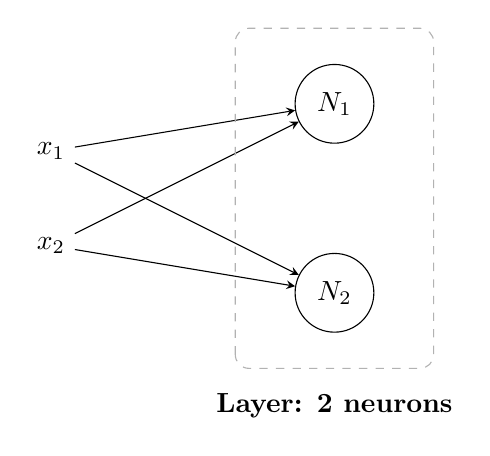
\begin{tikzpicture}[x=1.8cm, y=1.2cm, >=stealth]
    
    % Inputs
    \node at (0,2) (x1) {$x_1$};
    \node at (0,1) (x2) {$x_2$};
    
    % First neuron N1
    \node[circle,draw,minimum size=1cm] at (2,2.5) (N1) {$N_1$};
    \draw[->] (x1) -- (N1);
    \draw[->] (x2) -- (N1);
    
    % Second neuron N2
    \node[circle,draw,minimum size=1cm] at (2,0.5) (N2) {$N_2$};
    \draw[->] (x1) -- (N2);
    \draw[->] (x2) -- (N2);
    
    % Layer box
    \draw[dashed,rounded corners=5pt,gray!60] (1.3,-0.3) rectangle (2.7,3.3);
    \node at (2,-0.7) {\textbf{Layer: 2 neurons}};
    
    \end{tikzpicture}
    \caption{A layer groups multiple neurons — each with its own weights and bias — but sharing the same input.}
\end{figure}

\vspace{2em}

\section*{\fbox{\large What Is a Layer?}}

A \textbf{layer} is simply a collection of neurons that operate \textit{in parallel}.  
They all receive the same input vector, but each computes something slightly different.

\begin{itemize}
  \item Each neuron has its own weight vector and bias.
  \item Each neuron produces one output.
\end{itemize}

So here, with $N_1$ and $N_2$, we’ll get two outputs: $z_1$ and $z_2$.

\vspace{2em}

\section*{\fbox{\large Let’s Zoom In — Neuron by Neuron}}

\textbf{Neuron $N_1$} takes the input $(x_1, x_2)$ and computes:
\[
z_1 = W_{11} \cdot x_1 + W_{12} \cdot x_2 + b_1
\]

Where:
\begin{itemize}
  \item $W_{11}$ and $W_{12}$ are the weights of $N_1$,
  \item $b_1$ is its bias.
\end{itemize}

\textbf{Neuron $N_2$} does the exact same thing — but with different weights and bias:
\[
z_2 = W_{21} \cdot x_1 + W_{22} \cdot x_2 + b_2
\]

So even though they process the same input, the result is different — because their parameters are different.

\vspace{1em}

This is the power of layers: many neurons, one input, multiple outputs.

\vspace{2em}

\section*{\fbox{\large The Output Equation — Matrix Form}}

Now let’s write all of this in a single, elegant expression:

\[
\begin{bmatrix}
z_1 \\
z_2
\end{bmatrix}
=
\begin{bmatrix}
W_{11} & W_{12} \\
W_{21} & W_{22}
\end{bmatrix}
\begin{bmatrix}
x_1 \\
x_2
\end{bmatrix}
+
\begin{bmatrix}
b_1 \\
b_2
\end{bmatrix}
\]

Or, more compactly:
\[
Z = W x + b
\]

\vspace{1em}

\begin{tcolorbox}[colback=blue!5, colframe=blue!80!black, title=Notation Guide]
\begin{itemize}
  \item $x$ is the input vector (shared by all neurons),
  \item $W$ is the weight matrix — each row is a neuron,
  \item $b$ is the bias vector,
  \item $Z$ is the output vector of the layer.
\end{itemize}
\end{tcolorbox}

\vspace{1em}

\begin{tcolorbox}[colback=green!5!white, colframe=green!50!black, title=Key Insight]
The matrix equation $Z = Wx + b$ allows us to compute the output of the whole layer in one step —  
it’s the vectorized form of everything we just did manually.
\end{tcolorbox}

\section*{\fbox{\Large Activation Function}}

We’re almost there.  
Now that our neurons have computed their raw outputs $z_1$ and $z_2$, we apply a final transformation:

\begin{center}
    \textbf{The activation function.}
\end{center}

\vspace{0.5em}

Why?  
Because we want to introduce \textbf{non-linearity} into our model —  
so it can learn complex patterns, not just straight lines.

\vspace{1em}

\begin{tcolorbox}[colback=blue!5, colframe=blue!80!black, title=Sigmoid Activation Function]
The sigmoid is a classic choice:
\[
a(z) = \frac{1}{1 + e^{-z}}
\]

It maps any real number to a value between $0$ and $1$.  
Perfect when we want to interpret outputs as probabilities.
\end{tcolorbox}

\vspace{1.5em}

We apply the sigmoid to each neuron's output individually:

\[
A = a(Z)
\quad \Rightarrow \quad
\begin{bmatrix}
a_1 \\
a_2
\end{bmatrix}
=
\begin{bmatrix}
a(z_1) \\
a(z_2)
\end{bmatrix}
=
\begin{bmatrix}
\frac{1}{1 + e^{-z_1}} \\
\frac{1}{1 + e^{-z_2}}
\end{bmatrix}
\]

Here, $a_1$ and $a_2$ are the \textbf{activated outputs} of neurons $N_1$ and $N_2$.

\vspace{1.5em}

\begin{tcolorbox}[colback=green!5, colframe=green!60!black, title=Key Insight]
Each neuron computes its own linear combination: $z = Wx + b$  
Then applies an activation: $a = \sigma(z)$  
The result: nonlinear, learnable, expressive outputs.
\end{tcolorbox}

\vspace{2em}

\section*{\fbox{\Large Visual Summary}}

Here is what we’ve just built — a layer of two neurons with activation functions:

\vspace{1em}

\begin{figure}[H]
\centering
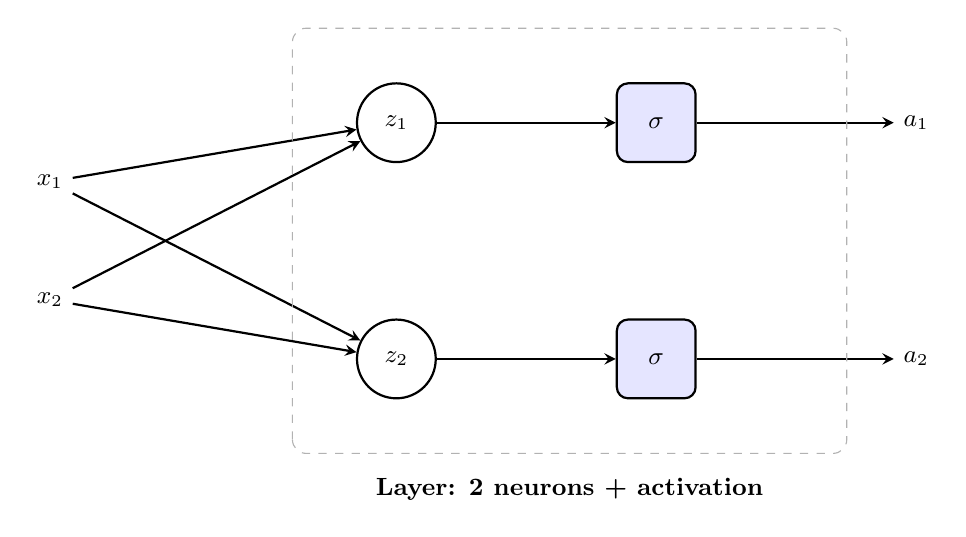
\begin{tikzpicture}[x=2.2cm, y=1.5cm, >=stealth, every node/.style={font=\small}]

% Input nodes
\node at (0,2) (x1) {$x_1$};
\node at (0,1) (x2) {$x_2$};

% Neurons z (linear)
\node[circle,draw,minimum size=1cm,thick] at (2,2.5) (N1) {$z_1$};
\node[circle,draw,minimum size=1cm,thick] at (2,0.5) (N2) {$z_2$};

% Activation function blocks
\node[rectangle,draw,minimum height=1cm,minimum width=1cm,thick,rounded corners=4pt,fill=blue!10] at (3.5,2.5) (A1) {$\sigma$};
\node[rectangle,draw,minimum height=1cm,minimum width=1cm,thick,rounded corners=4pt,fill=blue!10] at (3.5,0.5) (A2) {$\sigma$};

% Activated outputs
\node at (5,2.5) (a1) {$a_1$};
\node at (5,0.5) (a2) {$a_2$};

% Connections: x to z
\draw[->,thick] (x1) -- (N1);
\draw[->,thick] (x2) -- (N1);
\draw[->,thick] (x1) -- (N2);
\draw[->,thick] (x2) -- (N2);

% Connections: z to sigma
\draw[->,thick] (N1) -- (A1);
\draw[->,thick] (N2) -- (A2);

% Connections: sigma to activated output
\draw[->,thick] (A1) -- (a1);
\draw[->,thick] (A2) -- (a2);

% Layer box
\draw[dashed,rounded corners=5pt,gray!60] (1.4,-0.3) rectangle (4.6,3.3);
\node at (3,-0.6) {\textbf{Layer: 2 neurons + activation}};
\end{tikzpicture}
\caption{Each neuron computes $z = Wx + b$, then applies $\sigma(z)$ to produce its final output $a$.}
\end{figure}


\vspace{2em}

\section*{\fbox{\Large Very Important}}

\begin{quote}
\textbf{The outputs of the activation function are the true outputs of the layer.}  

In our case, we now have two activated outputs:  
\[
\boxed{a_1 \quad \text{and} \quad a_2}
\]
These form the output vector of the first layer.
\end{quote}

\section*{\fbox{\Large Adding Neurons in the Layer}}

Let’s say we want more power.  
What’s stopping us from adding more neurons to the layer?

\begin{tcolorbox}[colback=blue!5!white, colframe=blue!80!black, title=Answer:]
\textbf{Nothing.} We just add more rows to the weight matrix, and more entries in the bias vector.
\end{tcolorbox}

\vspace{1em}

Here’s what that looks like:

\[
W =
\begin{bmatrix}
W_{11} & W_{12} \\
W_{21} & W_{22} \\
W_{31} & W_{32}
\end{bmatrix}
\quad \text{and} \quad
b =
\begin{bmatrix}
b_1 \\
b_2 \\
b_3
\end{bmatrix}
\]

Same input $x$, same formula:
\[
Z = W x + b
\]

Now, the output becomes:

\[
\begin{bmatrix}
z_1 \\
z_2 \\
z_3
\end{bmatrix}
=
\begin{bmatrix}
W_{11} & W_{12} \\
W_{21} & W_{22} \\
W_{31} & W_{32}
\end{bmatrix}
\begin{bmatrix}
x_1 \\
x_2
\end{bmatrix}
+
\begin{bmatrix}
b_1 \\
b_2 \\
b_3
\end{bmatrix}
\]

Each new row corresponds to a new neuron, with its own weights and bias.  
The logic remains exactly the same.

\vspace{1em}

\begin{quote}
\textbf{We can add 3, 10, 100 neurons — as many as we want — and the equation stays the same.}
\end{quote}

\vspace{2em}

\begin{figure}[H]
\centering
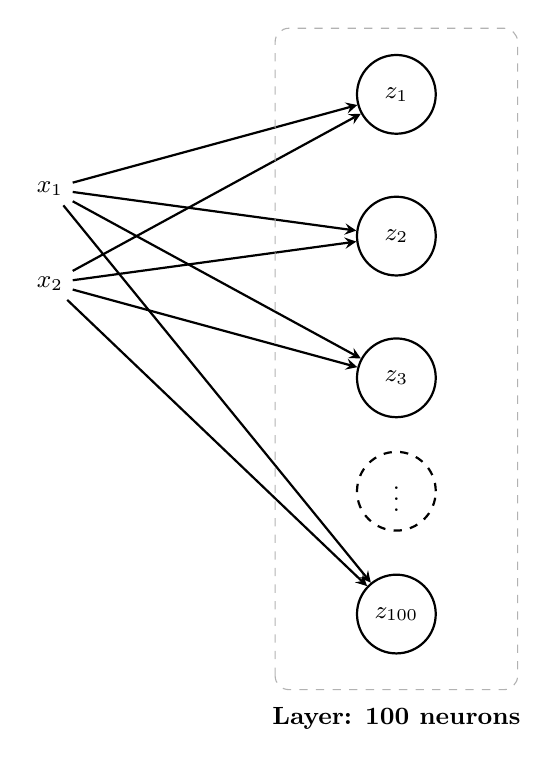
\begin{tikzpicture}[x=2.2cm, y=1.2cm, >=stealth, every node/.style={font=\small}]

% Inputs
\node at (0,3) (x1) {$x_1$};
\node at (0,2) (x2) {$x_2$};

% Neurons z (linear)
\node[circle,draw,minimum size=1cm,thick] at (2,4) (N1) {$z_1$};
\node[circle,draw,minimum size=1cm,thick] at (2,2.5) (N2) {$z_2$};
\node[circle,draw,minimum size=1cm,thick] at (2,1) (N3) {$z_3$};
\node[circle,draw,minimum size=1cm,thick,dashed] at (2,-0.2) (Ndots) {$\vdots$};
\node[circle,draw,minimum size=1cm,thick] at (2,-1.5) (N6) {$z_{100}$};

% Connections (show to 3 neurons only)
\foreach \target in {N1,N2,N3,N6} {
    \draw[->,thick] (x1) -- (\target);
    \draw[->,thick] (x2) -- (\target);
}

% Layer box
\draw[dashed,rounded corners=5pt,gray!60] (1.3,-2.3) rectangle (2.7,4.7);
\node at (2,-2.6) {\textbf{Layer: 100 neurons}};
\end{tikzpicture}
\caption{A layer with 100 neurons — each receiving the same input, but with its own weights and bias.}
\end{figure}
\section*{\fbox{\Large A Layer is a Collection of Neurons}}

Let’s take a step back and reframe what a layer really is.

A \textbf{layer} is just a collection of neurons working in parallel.  
It takes an input, and produces multiple outputs — one from each neuron.  

\begin{tcolorbox}[colback=green!5, colframe=green!50!black, title=Analogy]
You can think of a layer as one giant neuron —  
but made of many smaller neurons, each with its own weights and bias.
\end{tcolorbox}

\vspace{1em}

For now, we’re working with two neurons in our first layer.

We now introduce the notation for layers explicitly.  
The output of the first layer — after applying the activation — is written as:

\[
A = A_1 = 
\begin{bmatrix}
a_1 \\
a_2
\end{bmatrix}
= a(Z_1) =
\begin{bmatrix}
a(z_1) \\
a(z_2)
\end{bmatrix}
\]

Where:
\begin{itemize}
  \item $Z_1$ is the pre-activation output of the first layer (before sigmoid),
  \item $A_1$ is the activated output of the first layer,
  \item $a_1$ and $a_2$ are the outputs of neurons $N_1$ and $N_2$ after activation.
\end{itemize}

\vspace{2em}

\section*{\fbox{\Large Adding a Second Layer}}

Now, something exciting happens.

We’re no longer going to feed the raw input $x$ to the layer —  
we’re going to feed it the output of the previous layer: $A_1$.

\begin{tcolorbox}[colback=blue!5, colframe=blue!80!black, title=Deep Architecture]
\begin{itemize}
    \item The first layer takes the original input $x$ and produces $A_1$.
    \item The second layer takes $A_1$ as input and produces $A_2$.
\end{itemize}
\end{tcolorbox}

\vspace{1em}

Let’s keep it simple for now.  
\textbf{We’ll add just one neuron in the second layer.}

This neuron will:
\begin{itemize}
  \item Take $a_1$ and $a_2$ as inputs,
  \item Apply its own weights and bias,
  \item Produce a pre-activation $z_3$,
  \item Then apply the activation to get $a_3$.
\end{itemize}

\[
z_3 = W_{31} \cdot a_1 + W_{32} \cdot a_2 + b_3
\quad \Rightarrow \quad
a_3 = \sigma(z_3)
\]

So now we have:

\[
A_2 =
\begin{bmatrix}
a_3
\end{bmatrix}
\]

\vspace{1em}

\begin{tcolorbox}[colback=yellow!5, colframe=yellow!60!black, title=Key Insight]
Each new layer takes the output of the previous layer as input.  
This stacking is what gives neural networks their depth — and power.
\end{tcolorbox}
\begin{figure}[H]
\centering
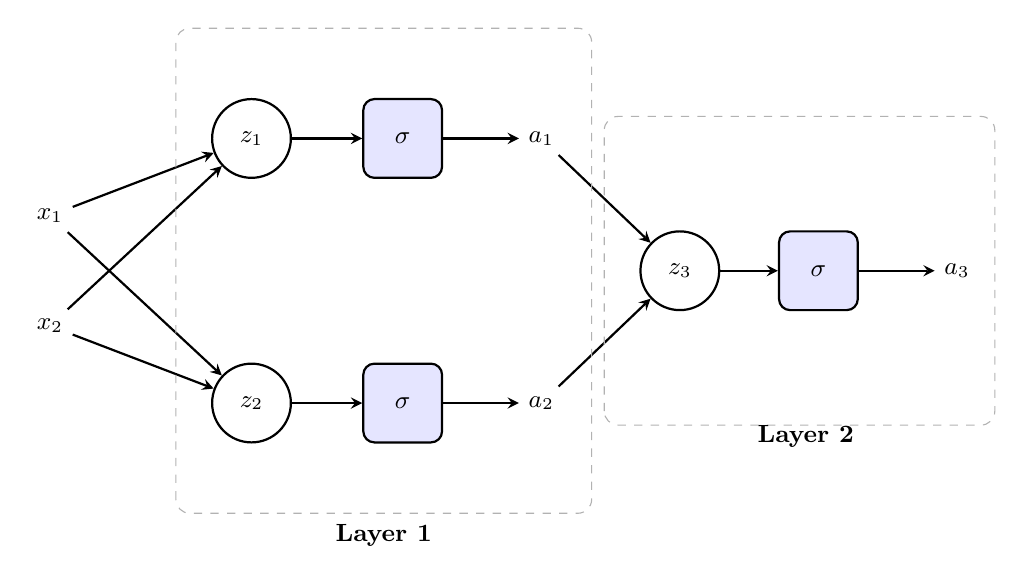
\begin{tikzpicture}[x=1.6cm, y=1.4cm, >=stealth, every node/.style={font=\small}]

% Inputs
\node at (0,3) (x1) {$x_1$};
\node at (0,2) (x2) {$x_2$};

% Hidden layer z
\node[circle,draw,thick,minimum size=1cm] at (1.6,3.7) (z1) {$z_1$};
\node[circle,draw,thick,minimum size=1cm] at (1.6,1.3) (z2) {$z_2$};

% Activations a1 and a2
\node[rectangle,draw,rounded corners=4pt,thick,fill=blue!10,minimum size=1cm] at (2.8,3.7) (a1) {$\sigma$};
\node[rectangle,draw,rounded corners=4pt,thick,fill=blue!10,minimum size=1cm] at (2.8,1.3) (a2) {$\sigma$};

% Activated outputs
\node at (3.9,3.7) (a1_out) {$a_1$};
\node at (3.9,1.3) (a2_out) {$a_2$};

% Second layer z3
\node[circle,draw,thick,minimum size=1cm] at (5,2.5) (z3) {$z_3$};

% Activation a3
\node[rectangle,draw,rounded corners=4pt,thick,fill=blue!10,minimum size=1cm] at (6.1,2.5) (a3) {$\sigma$};

% Output a3
\node at (7.2,2.5) (a3_out) {$a_3$};

% Connections: input to layer 1
\foreach \target in {z1,z2} {
  \draw[->,thick] (x1) -- (\target);
  \draw[->,thick] (x2) -- (\target);
}

% Connections: z to activation
\draw[->,thick] (z1) -- (a1);
\draw[->,thick] (z2) -- (a2);

% Connections: activation to a1_out
\draw[->,thick] (a1) -- (a1_out);
\draw[->,thick] (a2) -- (a2_out);

% Connections: a1 and a2 to z3
\draw[->,thick] (a1_out) -- (z3);
\draw[->,thick] (a2_out) -- (z3);

% z3 to a3 to final output
\draw[->,thick] (z3) -- (a3);
\draw[->,thick] (a3) -- (a3_out);

% Layer boxes
\draw[dashed,gray!60,rounded corners=5pt] (1,0.3) rectangle (4.3,4.7);
\node at (2.65,0.1) {\textbf{Layer 1}};

\draw[dashed,gray!60,rounded corners=5pt] (4.4,1.1) rectangle (7.5,3.9);
\node at (6,1) {\textbf{Layer 2}};

\end{tikzpicture}
\caption{A two-layer neural network: the output of Layer 1 becomes the input to Layer 2.}
\end{figure}


\section*{\fbox{\Large Second Layer Computation}}

We now know that the output of the first layer is:
\[
A_1 =
\begin{bmatrix}
a_1 \\
a_2
\end{bmatrix}
\]

Let’s feed this into the second layer.  
This time, we’ll work with a single neuron in the second layer.

\vspace{1em}

\begin{tcolorbox}[colback=blue!5!white, colframe=blue!80!black, title=Layer 2 Computation]
The second layer computes:
\[
Z_2 = W_2 A_1 + b_2
\]
Where:
\begin{itemize}
  \item $W_2$ is the weight matrix of the second layer,
  \item $A_1$ is the input (from the first layer),
  \item $b_2$ is the bias of the second layer.
\end{itemize}
\end{tcolorbox}

\vspace{1em}

Then we apply the activation function:
\[
A_2 = a(Z_2)
\]

Let’s look at a concrete example.  
Suppose we have:

\[
W_2 = \begin{bmatrix} w_{21} & w_{22} \end{bmatrix}, \quad
b_2 = \begin{bmatrix} b_3 \end{bmatrix}
\]

Then:
\[
Z_2 = 
\begin{bmatrix}
z_3
\end{bmatrix}
= W_2 A_1 + b_2 = 
\begin{bmatrix}
w_{21} & w_{22}
\end{bmatrix}
\begin{bmatrix}
a_1 \\
a_2
\end{bmatrix}
+
\begin{bmatrix}
b_3
\end{bmatrix}
\]

And the final activated output becomes:

\[
A_2 = 
\begin{bmatrix}
a_3
\end{bmatrix}
= a(Z_2) = 
\begin{bmatrix}
a(z_3)
\end{bmatrix}
= \begin{bmatrix}
\frac{1}{1 + e^{-z_3}}
\end{bmatrix}
\]

\vspace{2em}

This shows a full forward pass through a 2-layer neural network.  
From $x \rightarrow A_1 \rightarrow A_2$, the data flows forward — layer by layer —  
with weights, biases, and activations applied at each stage.

\vspace{1em}

\begin{tcolorbox}[colback=green!5, colframe=green!60!black, title=Key Insight]
Each layer is a clean block: linear operation ($Wx + b$) followed by a non-linearity ($a(z)$).  
Stacking these blocks is what builds a deep neural network.
\end{tcolorbox}
\section*{\fbox{\Large Adding More Neurons to the Second Layer}}

Why stop at one neuron?

We can easily add more neurons to the second layer by:

\begin{itemize}
  \item adding more \textbf{rows} to the weight matrix $W_2$,
  \item and more \textbf{entries} to the bias vector $b_2$.
\end{itemize}

\begin{tcolorbox}[colback=gray!5, colframe=gray!60!black, title={Same Logic, More Neurons}]
The matrix equation stays the same:
\[
Z_2 = W_2 A_1 + b_2
\]
\end{tcolorbox}

Let’s say we now have \textbf{three neurons} in the second layer.  
The output becomes:

\[
A_2 = 
\begin{bmatrix}
a_1 \\
a_2 \\
a_3
\end{bmatrix}
= a(Z_2) = 
a\left(
\begin{bmatrix}
z_1 \\
z_2 \\
z_3
\end{bmatrix}
\right)
=
\begin{bmatrix}
a(z_1) \\
a(z_2) \\
a(z_3)
\end{bmatrix}
\]

Each $z_i$ is computed using its own weights and bias:

\[
\begin{bmatrix}
z_1 \\
z_2 \\
z_3
\end{bmatrix}
=
\begin{bmatrix}
W_{11} & W_{12} \\
W_{21} & W_{22} \\
W_{31} & W_{32}
\end{bmatrix}
\begin{bmatrix}
a_1 \\
a_2
\end{bmatrix}
+
\begin{bmatrix}
b_1 \\
b_2 \\
b_3
\end{bmatrix}
\]

\begin{tcolorbox}[colback=green!5, colframe=green!60!black, title=Reminder]
Each row of $W_2$ corresponds to one neuron in the layer.  
Each neuron gets the full input $A_1$ but transforms it differently.
\end{tcolorbox}

\vspace{2em}

\section*{\fbox{\Large Visual Recap}}

Here’s what we’ve just built — a second layer with three neurons:

\begin{figure}[H]
\centering
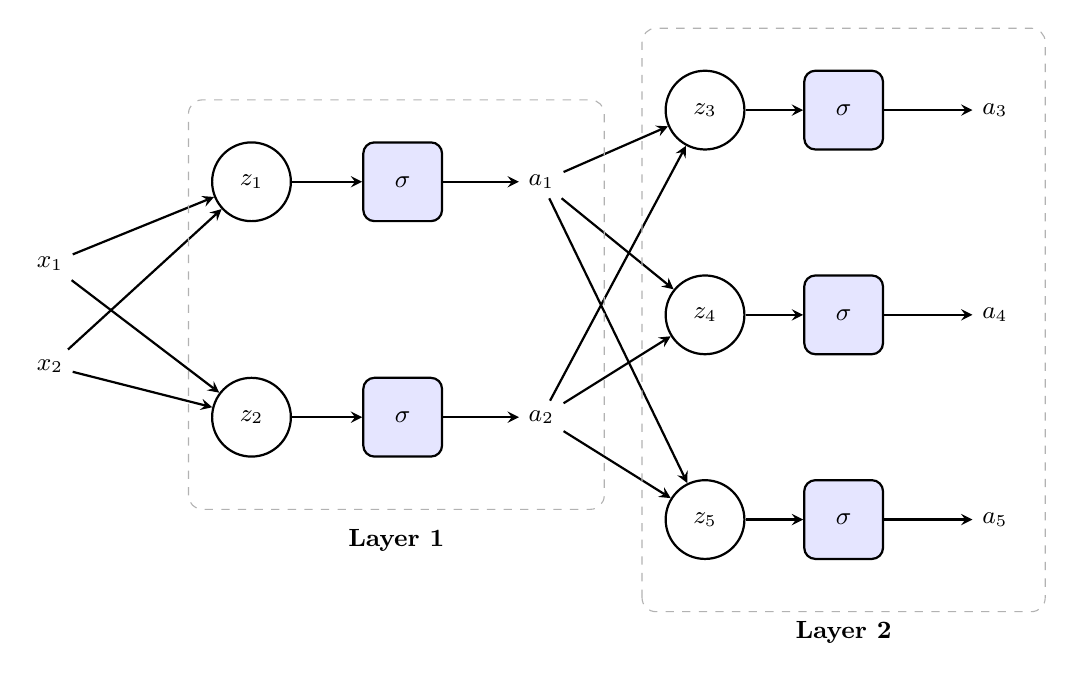
\begin{tikzpicture}[x=1.6cm, y=1.3cm, >=stealth, every node/.style={font=\small}]

% Inputs
\node at (0,3) (x1) {$x_1$};
\node at (0,2) (x2) {$x_2$};

% Layer 1 z
\node[circle,draw,thick,minimum size=1cm] at (1.6,3.8) (z1) {$z_1$};
\node[circle,draw,thick,minimum size=1cm] at (1.6,1.5) (z2) {$z_2$};

% Activations a1
\node[rectangle,draw,rounded corners=4pt,thick,fill=blue!10,minimum size=1cm] at (2.8,3.8) (a1) {$\sigma$};
\node[rectangle,draw,rounded corners=4pt,thick,fill=blue!10,minimum size=1cm] at (2.8,1.5) (a2) {$\sigma$};

% Layer 1 outputs
\node at (3.9,3.8) (a1_out) {$a_1$};
\node at (3.9,1.5) (a2_out) {$a_2$};

% Layer 2 z neurons
\node[circle,draw,thick,minimum size=1cm] at (5.2,4.5) (z3) {$z_3$};
\node[circle,draw,thick,minimum size=1cm] at (5.2,2.5) (z4) {$z_4$};
\node[circle,draw,thick,minimum size=1cm] at (5.2,0.5) (z5) {$z_5$};

% Activations a3
\node[rectangle,draw,rounded corners=4pt,thick,fill=blue!10,minimum size=1cm] at (6.3,4.5) (a3) {$\sigma$};
\node[rectangle,draw,rounded corners=4pt,thick,fill=blue!10,minimum size=1cm] at (6.3,2.5) (a4) {$\sigma$};
\node[rectangle,draw,rounded corners=4pt,thick,fill=blue!10,minimum size=1cm] at (6.3,0.5) (a5) {$\sigma$};

% Outputs a3, a4, a5
\node at (7.5,4.5) (a3_out) {$a_3$};
\node at (7.5,2.5) (a4_out) {$a_4$};
\node at (7.5,0.5) (a5_out) {$a_5$};

% Connections: x to z1, z2
\foreach \target in {z1,z2} {
  \draw[->,thick] (x1) -- (\target);
  \draw[->,thick] (x2) -- (\target);
}

% Connections: z to activation
\draw[->,thick] (z1) -- (a1);
\draw[->,thick] (z2) -- (a2);

% Activation to output
\draw[->,thick] (a1) -- (a1_out);
\draw[->,thick] (a2) -- (a2_out);

% Layer 1 to Layer 2 z-neurons
\foreach \dest in {z3,z4,z5} {
  \draw[->,thick] (a1_out) -- (\dest);
  \draw[->,thick] (a2_out) -- (\dest);
}

% z to sigma
\draw[->,thick] (z3) -- (a3);
\draw[->,thick] (z4) -- (a4);
\draw[->,thick] (z5) -- (a5);

% sigma to output
\draw[->,thick] (a3) -- (a3_out);
\draw[->,thick] (a4) -- (a4_out);
\draw[->,thick] (a5) -- (a5_out);

% Layer boxes
\draw[dashed,gray!60,rounded corners=5pt] (1.1,0.6) rectangle (4.4,4.6);
\node at (2.75,0.3) {\textbf{Layer 1}};

\draw[dashed,gray!60,rounded corners=5pt] (4.7,-0.4) rectangle (7.9,5.3);
\node at (6.3,-0.6) {\textbf{Layer 2}};

\end{tikzpicture}
\caption{Two-layer neural network: 2 neurons in Layer 1, 3 neurons in Layer 2.}
\end{figure}


\section*{\fbox{\Large Adding a Layer}}

\vspace{0.5em}

\textbf{Key distinction:}

\begin{itemize}
    \item To \textbf{add a neuron within a layer}, you simply add a new \textbf{row} to the weight matrix and a new \textbf{entry} to the bias vector.
    \item To \textbf{add a new layer}, you introduce an entirely new \textbf{weight matrix} and a new \textbf{bias vector}.
\end{itemize}

\vspace{1em}
\section*{\fbox{\Large Output Layer and Final Output}}

The \textbf{output layer} is the last layer of the neural network.  
It takes as input the output of the last hidden layer — and produces the final prediction.

\vspace{1em}

Let’s say we use the following weight matrix and bias vector:

\[
W_3 = 
\begin{bmatrix}
w_{11} & w_{12} & w_{13}
\end{bmatrix}
\quad \text{and} \quad
b_3 = 
\begin{bmatrix}
b_1
\end{bmatrix}
\]

We compute the pre-activation of the output neuron:

\[
Z_3 = 
\begin{bmatrix}
z_1
\end{bmatrix}
= W_3 A_2 + b_3 = 
\begin{bmatrix}
w_{11} & w_{12} & w_{13}
\end{bmatrix}
\begin{bmatrix}
a_1 \\
a_2 \\
a_3
\end{bmatrix}
+
\begin{bmatrix}
b_1
\end{bmatrix}
\]

Then we apply the activation function (here: sigmoid) to get the final prediction:

\[
A_3 = a(Z_3) =
\begin{bmatrix}
\frac{1}{1 + e^{-z_1}}
\end{bmatrix}
\]

\vspace{2em}

\begin{figure}[H]
\centering
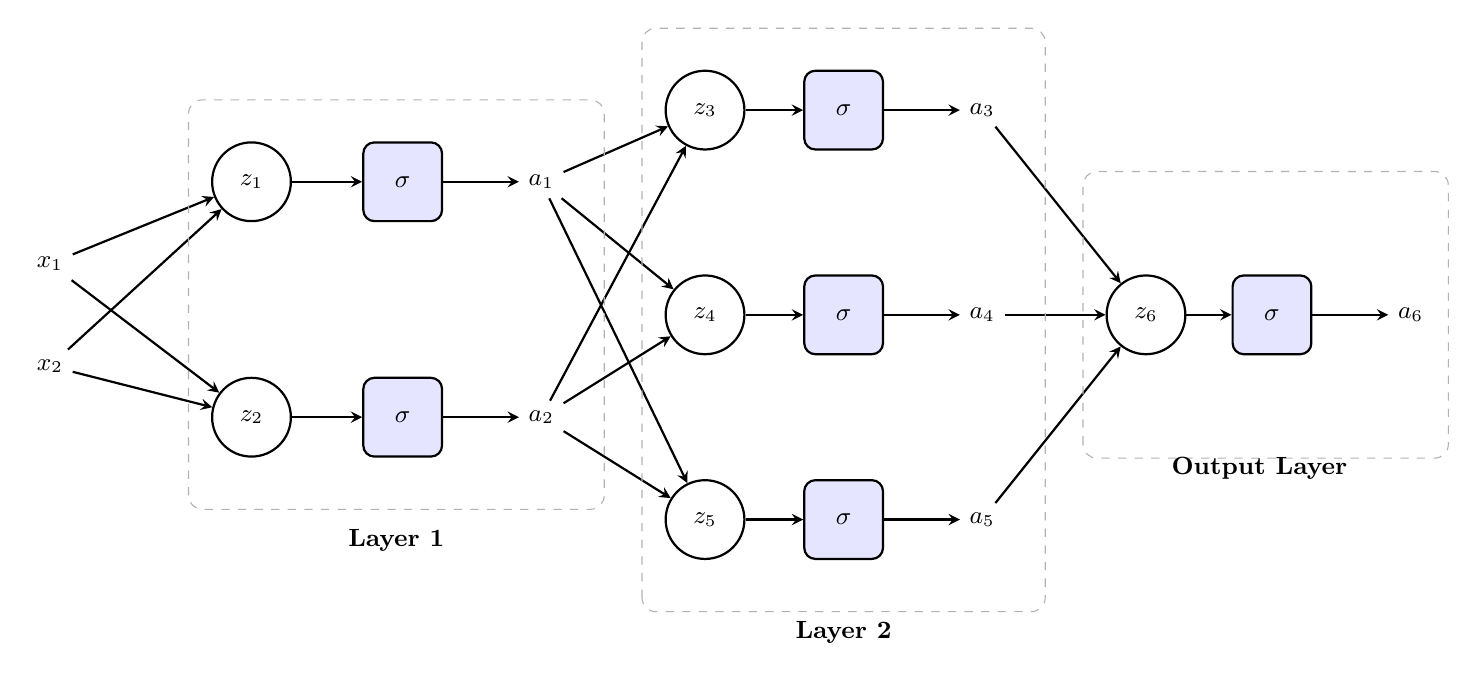
\begin{tikzpicture}[x=1.6cm, y=1.3cm, >=stealth, every node/.style={font=\small}]

% Inputs
\node at (0,3) (x1) {$x_1$};
\node at (0,2) (x2) {$x_2$};

% Layer 1 z
\node[circle,draw,thick,minimum size=1cm] at (1.6,3.8) (z1) {$z_1$};
\node[circle,draw,thick,minimum size=1cm] at (1.6,1.5) (z2) {$z_2$};

% Activations a1
\node[rectangle,draw,rounded corners=4pt,thick,fill=blue!10,minimum size=1cm] at (2.8,3.8) (a1) {$\sigma$};
\node[rectangle,draw,rounded corners=4pt,thick,fill=blue!10,minimum size=1cm] at (2.8,1.5) (a2) {$\sigma$};

% Outputs of layer 1
\node at (3.9,3.8) (a1_out) {$a_1$};
\node at (3.9,1.5) (a2_out) {$a_2$};

% Layer 2 z neurons
\node[circle,draw,thick,minimum size=1cm] at (5.2,4.5) (z3) {$z_3$};
\node[circle,draw,thick,minimum size=1cm] at (5.2,2.5) (z4) {$z_4$};
\node[circle,draw,thick,minimum size=1cm] at (5.2,0.5) (z5) {$z_5$};

% Activations a3
\node[rectangle,draw,rounded corners=4pt,thick,fill=blue!10,minimum size=1cm] at (6.3,4.5) (a3) {$\sigma$};
\node[rectangle,draw,rounded corners=4pt,thick,fill=blue!10,minimum size=1cm] at (6.3,2.5) (a4) {$\sigma$};
\node[rectangle,draw,rounded corners=4pt,thick,fill=blue!10,minimum size=1cm] at (6.3,0.5) (a5) {$\sigma$};

% Outputs of layer 2
\node at (7.4,4.5) (a3_out) {$a_3$};
\node at (7.4,2.5) (a4_out) {$a_4$};
\node at (7.4,0.5) (a5_out) {$a_5$};

% Output layer z neuron
\node[circle,draw,thick,minimum size=1cm] at (8.7,2.5) (z6) {$z_6$};

% Activation
\node[rectangle,draw,rounded corners=4pt,thick,fill=blue!10,minimum size=1cm] at (9.7,2.5) (a6) {$\sigma$};

% Final output
\node at (10.8,2.5) (a6_out) {$a_6$};

% Connections
\foreach \target in {z1,z2} {
  \draw[->,thick] (x1) -- (\target);
  \draw[->,thick] (x2) -- (\target);
}
\draw[->,thick] (z1) -- (a1);
\draw[->,thick] (z2) -- (a2);
\draw[->,thick] (a1) -- (a1_out);
\draw[->,thick] (a2) -- (a2_out);
\foreach \target in {z3,z4,z5} {
  \draw[->,thick] (a1_out) -- (\target);
  \draw[->,thick] (a2_out) -- (\target);
}
\draw[->,thick] (z3) -- (a3);
\draw[->,thick] (z4) -- (a4);
\draw[->,thick] (z5) -- (a5);
\draw[->,thick] (a3) -- (a3_out);
\draw[->,thick] (a4) -- (a4_out);
\draw[->,thick] (a5) -- (a5_out);

\foreach \src in {a3_out,a4_out,a5_out} {
  \draw[->,thick] (\src) -- (z6);
}
\draw[->,thick] (z6) -- (a6);
\draw[->,thick] (a6) -- (a6_out);

% Layer boxes
\draw[dashed,gray!60,rounded corners=5pt] (1.1,0.6) rectangle (4.4,4.6);
\node at (2.75,0.3) {\textbf{Layer 1}};

\draw[dashed,gray!60,rounded corners=5pt] (4.7,-0.4) rectangle (7.9,5.3);
\node at (6.3,-0.6) {\textbf{Layer 2}};

\draw[dashed,gray!60,rounded corners=5pt] (8.2,1.1) rectangle (11.1,3.9);
\node at (9.6,1) {\textbf{Output Layer}};

\end{tikzpicture}
\caption{Complete neural network: 2 inputs, 2 hidden layers, 1 output neuron.}
\end{figure}

\vspace{1em}

\section*{\fbox{\Large Summary}}

\vspace{-0.5em}

\begin{itemize}
    \item \textbf{Adding a neuron} = add a row to $W$, and an element to $b$.
    \item \textbf{Adding a layer} = create a new $W_i$ and $b_i$.
\end{itemize}

Each layer performs the same core sequence:

\vspace{0.5em}

\begin{tcolorbox}[colback=green!5, colframe=green!60!black, title=Layer Computation — General Rule]
\[
\text{Input:} \quad A_{i-1}
\]
\[
\text{Linear combination:} \quad Z_i = W_i A_{i-1} + b_i
\]
\[
\text{Activation:} \quad A_i = a(Z_i)
\]
\end{tcolorbox}

\vspace{1em}

\textbf{Why matrices?}  
Because they allow us to compute all neurons’ operations at once —  
fast, in parallel, and efficiently on modern hardware.


\section*{\fbox{\Large Forward Propagation}}

Forward propagation is the process of passing the input through the entire network —  
from the input layer, through all hidden layers, to the final output.

\vspace{0.5em}

At each step, the same logic applies:

\begin{itemize}
    \item Apply a \textbf{linear operation} ($Z = W A + b$)
    \item Apply an \textbf{activation function} ($A = \sigma(Z)$)
\end{itemize}

This continues until we reach the final output:

\[
A_3 = \text{network prediction}
\]

\vspace{2em}

\section*{\fbox{\Large Training via Backpropagation}}

Once we compute the output, we want to train the network —  
that is, adjust the weights and biases to reduce the prediction error.

\vspace{0.5em}

To train the network, we follow these steps:

\begin{enumerate}
    \item Define a \textbf{loss function} (such as log-loss)
    \item Compute the \textbf{gradient of the loss} with respect to each parameter
    \item Update the weights and biases using \textbf{gradient descent}
\end{enumerate}

\vspace{1em}

From our earlier notebook (for a single neuron), we saw:

\[
\frac{\partial \mathcal{L}}{\partial w_1} = -\frac{x_1}{m} \sum_i (y_i - a_i)
\quad\quad
\frac{\partial \mathcal{L}}{\partial w_2} = -\frac{x_2}{m} \sum_i (y_i - a_i)
\quad\quad
\frac{\partial \mathcal{L}}{\partial b} = -\frac{1}{m} \sum_i (y_i - a_i)
\]

Remember, we derived these expressions using the chain rule.

\vspace{1em}

\begin{tcolorbox}[colback=blue!5, colframe=blue!80!black, title=Now We Scale Up]
We will do the exact same thing here — but with \textbf{matrices}.
\end{tcolorbox}

\vspace{1em}
\subsection*{\fbox{\large Goal: Compute the Gradients}}

Let’s focus on the following parameters:

\begin{itemize}
  \item $W_1$, $b_1$ — parameters of the first layer
  \item $W_2$, $b_2$ — parameters of the second layer
\end{itemize}

Our goal is to understand how much each parameter influences the loss function.  
In other words, we want to compute:

\[
\frac{\partial \mathcal{L}}{\partial W_1}, \quad
\frac{\partial \mathcal{L}}{\partial b_1}, \quad
\frac{\partial \mathcal{L}}{\partial W_2}, \quad
\frac{\partial \mathcal{L}}{\partial b_2}
\]

As before — like we did in the perceptron model — we will use the \textbf{chain rule}.  
This time, however, we will apply it step by step through the layers of a deep network.

\vspace{1em}

\begin{tcolorbox}[colback=yellow!5, colframe=yellow!50!black, title=Before We Start]
\textbf{Read carefully. This is the foundation of the entire backward pass.}

You don’t need to memorize equations — but you must understand the logic.  
It’s all about how the functions are connected, and how parameters influence outputs.

If you get that, you’ll understand every neural network.
\end{tcolorbox}

\vspace{1.5em}

\subsection*{\fbox{\large Summary of the Network Functions}}

\vspace{0.5em}

\textbf{First Layer:}
\begin{itemize}
    \item Linear transformation:
    \[
    Z_1 = W_1 X + b_1
    \]
    \item Activation:
    \[
    A_1 = \frac{1}{1 + e^{-Z_1}}
    \]
\end{itemize}

\vspace{0.5em}

\textbf{Second Layer (Last Hidden Layer):}
\begin{itemize}
    \item Linear transformation:
    \[
    Z_2 = W_2 A_1 + b_2
    \]
    \textit{Important:} Here, the input is $A_1$, not the original input $X$.

    \item Activation:
    \[
    A_2 = \frac{1}{1 + e^{-Z_2}}
    \]

    \item Loss function:
    \[
    \mathcal{L} = -\frac{1}{m} \sum \left( y \log A_2 + (1 - y) \log(1 - A_2) \right)
    \]
    \textit{We compute the loss using $A_2$, the output of the last layer — not $A_1$.}
\end{itemize}

\section*{\fbox{\Large Important}}

Finding the gradients means identifying how the loss $\mathcal{L}$ depends on each parameter of the network.

But as you’ve already seen, the \textbf{entry point} between the loss $\mathcal{L}$ and the rest of the network is the output of the last layer — namely, $A_2$.

So even if we want to compute the gradients of the parameters in the \textit{first layer},  
we must first pass through the \textit{second layer}.

\vspace{0.5em}

\begin{tcolorbox}[colback=green!5!white, colframe=green!60!black, title=Key Insight]
This is the core principle of backpropagation:

\textbf{We must go backward through the network — layer by layer — to compute the gradients.}
\end{tcolorbox}

\vspace{0.5em}

And when you think about it, it actually makes perfect sense.  
This is the whole point of deep learning: the model builds up its complexity layer after layer.  
So naturally, we need to go back down that stack to understand how each parameter affects the final outcome.

\vspace{2em}

\section*{\fbox{\Large Gradients for the Layer Just Before the Output}}

Let’s now compute the gradients for the second layer, using the chain rule.

\[
\begin{aligned}
\frac{\partial \mathcal{L}}{\partial W_2} &= 
\frac{\partial \mathcal{L}}{\partial A_2} \cdot 
\frac{\partial A_2}{\partial Z_2} \cdot 
\frac{\partial Z_2}{\partial W_2} \\[1em]
\frac{\partial \mathcal{L}}{\partial b_2} &= 
\frac{\partial \mathcal{L}}{\partial A_2} \cdot 
\frac{\partial A_2}{\partial Z_2} \cdot 
\frac{\partial Z_2}{\partial b_2}
\end{aligned}
\]

Let’s break this down:

\begin{itemize}
    \item $\frac{\partial \mathcal{L}}{\partial A_2}$ is the gradient of the loss with respect to the network output
    \item $\frac{\partial A_2}{\partial Z_2}$ is the derivative of the activation function (sigmoid)
    \item $\frac{\partial Z_2}{\partial W_2}$ and $\frac{\partial Z_2}{\partial b_2}$ are the local gradients of the model
\end{itemize}

\vspace{0.5em}

Since the first two terms appear identically in both equations, we define:

\[
dZ_2 = \frac{\partial \mathcal{L}}{\partial A_2} \cdot \frac{\partial A_2}{\partial Z_2}
\]

Then the gradients simplify to:

\[
\begin{aligned}
\frac{\partial \mathcal{L}}{\partial W_2} &= dZ_2 \cdot \frac{\partial Z_2}{\partial W_2} \\
\frac{\partial \mathcal{L}}{\partial b_2} &= dZ_2 \cdot \frac{\partial Z_2}{\partial b_2}
\end{aligned}
\]

\section*{\fbox{\Large For the First Layer}}

Let’s now focus on computing the gradients with respect to the parameters of the \textbf{first layer}.

Using the chain rule:

\[
\begin{aligned}
\frac{\partial \mathcal{L}}{\partial W_1} &= 
\frac{\partial \mathcal{L}}{\partial A_1} \cdot 
\frac{\partial A_1}{\partial Z_1} \cdot 
\frac{\partial Z_1}{\partial W_1} \\[1em]
\frac{\partial \mathcal{L}}{\partial b_1} &= 
\frac{\partial \mathcal{L}}{\partial A_1} \cdot 
\frac{\partial A_1}{\partial Z_1} \cdot 
\frac{\partial Z_1}{\partial b_1}
\end{aligned}
\]

Where:
\begin{itemize}
    \item $\frac{\partial \mathcal{L}}{\partial A_1}$ is the gradient of the loss with respect to the output of the first layer
    \item $\frac{\partial A_1}{\partial Z_1}$ is the derivative of the activation function
    \item $\frac{\partial Z_1}{\partial W_1}$ and $\frac{\partial Z_1}{\partial b_1}$ are the local gradients of the linear model
\end{itemize}

But — as we said before — there's a crucial observation here:

\vspace{0.5em}
\textit{There is no direct link between the loss $\mathcal{L}$ and the output $A_1$ of the first layer.}  
To compute this gradient, we must go through the second layer — just like the signal does in the forward pass.

\vspace{1em}

\begin{tcolorbox}[colback=yellow!5, colframe=yellow!50!black, title=Pause and Think]
\textbf{How do we relate the second layer to the first?}  
What is the variable that connects both layers?

Take a moment and try to identify the link yourself.
\end{tcolorbox}

\vspace{1em}

The answer?

It’s in the equation:

\[
Z_2 = W_2 A_1 + b_2
\]

This shows that $A_1$ is the input to the second layer.  
So to compute $\frac{\partial \mathcal{L}}{\partial A_1}$, we apply the chain rule again:

\[
\frac{\partial \mathcal{L}}{\partial A_1} = 
\frac{\partial \mathcal{L}}{\partial A_2} \cdot 
\frac{\partial A_2}{\partial Z_2} \cdot 
\frac{\partial Z_2}{\partial A_1}
\]

\vspace{1em}

\begin{tcolorbox}[colback=green!5!white, colframe=green!60!black, title=What Just Happened]
We found a way to compute a gradient that had no direct path to the loss.

There is no direct dependency between $\mathcal{L}$ and $A_1$ —  
but by passing through $A_2$ and $Z_2$, we built the connection.

This is the heart of backpropagation:  
\textbf{working backward through the layers using the chain rule to connect everything.}
\end{tcolorbox}


\section*{\fbox{\Large Full Gradient Expression for the First Layer}}

Let’s now write the full expression for the gradients of the first layer, step by step, with the chain rule:

\[
\begin{aligned}
\frac{\partial \mathcal{L}}{\partial W_1} &= 
\frac{\partial \mathcal{L}}{\partial A_2} \cdot 
\frac{\partial A_2}{\partial Z_2} \cdot 
\frac{\partial Z_2}{\partial A_1} \cdot 
\frac{\partial A_1}{\partial Z_1} \cdot 
\frac{\partial Z_1}{\partial W_1} \\
\\
\frac{\partial \mathcal{L}}{\partial b_1} &= 
\frac{\partial \mathcal{L}}{\partial A_2} \cdot 
\frac{\partial A_2}{\partial Z_2} \cdot 
\frac{\partial Z_2}{\partial A_1} \cdot 
\frac{\partial A_1}{\partial Z_1} \cdot 
\frac{\partial Z_1}{\partial b_1}
\end{aligned}
\]

Let’s be honest: yes, that’s a long chain.  
But this is how deep learning works. And no, it’s not “just a few lines of code.”  
If it were simple, everyone would be doing it.

\begin{tcolorbox}[colback=blue!5, colframe=blue!80!black, title=Side Note]
Correction: everyone \emph{is} a “data scientist” on LinkedIn.  
But we’re here to understand what makes a \textbf{real and honest} one.
\end{tcolorbox}

\vspace{1em}

Still — we can simplify.

Just like we did earlier, we define:

\[
dZ_1 = 
\frac{\partial \mathcal{L}}{\partial A_2} \cdot 
\frac{\partial A_2}{\partial Z_2} \cdot 
\frac{\partial Z_2}{\partial A_1} \cdot 
\frac{\partial A_1}{\partial Z_1}
\]

But since we already defined:

\[
dZ_2 = \frac{\partial \mathcal{L}}{\partial A_2} \cdot \frac{\partial A_2}{\partial Z_2}
\]

We can write:

\[
dZ_1 = dZ_2 \cdot \frac{\partial Z_2}{\partial A_1} \cdot \frac{\partial A_1}{\partial Z_1}
\]

This gives us the final simplified expressions:

\[
\begin{aligned}
\frac{\partial \mathcal{L}}{\partial W_1} &= dZ_1 \cdot \frac{\partial Z_1}{\partial W_1} \\
\frac{\partial \mathcal{L}}{\partial b_1} &= dZ_1 \cdot \frac{\partial Z_1}{\partial b_1}
\end{aligned}
\]

\begin{tcolorbox}[colback=green!5!white, colframe=green!60!black, title=Structure of the Backward Pass]
Each gradient is built from:
\begin{itemize}
    \item the gradient from the next layer ($dZ_2$),
    \item the chain of derivatives that connects the current layer,
    \item and the local gradients of the linear model.
\end{itemize}
It’s structured, logical, and beautifully recursive.
\end{tcolorbox}


\section*{\fbox{\Large Summary of the Gradient Equations}}

Let’s recap what we want to compute during the backward pass:

\[
\begin{aligned}
\frac{\partial \mathcal{L}}{\partial W_2} &= dZ_2 \cdot \frac{\partial Z_2}{\partial W_2} \\
\frac{\partial \mathcal{L}}{\partial b_2} &= dZ_2 \cdot \frac{\partial Z_2}{\partial b_2} \\
\frac{\partial \mathcal{L}}{\partial W_1} &= dZ_1 \cdot \frac{\partial Z_1}{\partial W_1} \\
\frac{\partial \mathcal{L}}{\partial b_1} &= dZ_1 \cdot \frac{\partial Z_1}{\partial b_1}
\end{aligned}
\]

\vspace{1em}

To get there, we use:

\[
\begin{aligned}
dZ_2 &= \frac{\partial \mathcal{L}}{\partial A_2} \cdot \frac{\partial A_2}{\partial Z_2} \\
dZ_1 &= dZ_2 \cdot \frac{\partial Z_2}{\partial A_1} \cdot \frac{\partial A_1}{\partial Z_1}
\end{aligned}
\]

\vspace{1em}

\noindent
\textbf{Strategy:}
\begin{enumerate}
    \item Compute $dZ_2$ from the output layer.
    \item Use it to compute $\frac{\partial \mathcal{L}}{\partial W_2}$ and $\frac{\partial \mathcal{L}}{\partial b_2}$.
    \item Backpropagate to get $dZ_1$.
    \item Use it to compute $\frac{\partial \mathcal{L}}{\partial W_1}$ and $\frac{\partial \mathcal{L}}{\partial b_1}$.
\end{enumerate}

\vspace{2em}

\section*{\fbox{\Large Let’s Get to the Point}}

In theory, things are clear.  
In practice, there are no shortcuts.

If we want to understand how a neural network learns,  
we have to compute every gradient — one by one.

\textbf{This is the work.}

And now, we’re ready to do it.

\section*{\fbox{\Large 1. Computing \( dZ_2 \)}}

Let’s begin with the calculation of \( dZ_2 \) —  
because this term appears in both gradient expressions for the second layer,  
and we also need it to backpropagate further to the first layer.

We define:

\[
dZ_2 = \frac{\partial \mathcal{L}}{\partial A_2} \cdot \frac{\partial A_2}{\partial Z_2}
\]

Where:
\begin{itemize}
    \item \( \frac{\partial \mathcal{L}}{\partial A_2} \) is the gradient of the loss with respect to the output of the network,
    \item \( \frac{\partial A_2}{\partial Z_2} \) is the derivative of the sigmoid activation.
\end{itemize}

\vspace{1em}

Let’s compute the first term — the derivative of the loss.

\[
\frac{\partial \mathcal{L}}{\partial A_2} = ?
\]

\textbf{Wait… you don’t remember this?}

Come on — it’s the same expression we derived earlier in the previous notebook using the log-loss function.  
Fine. I’ll recap it but after that, you're on your own. I'm not your mom. For goodness' sake.

\vspace{1em}

\textbf{Loss function (log-loss):}

\[
\mathcal{L} = -\frac{1}{m} \sum_i \left( y_i \log A_2 + (1 - y_i) \log(1 - A_2) \right)
\]

We compute its derivative with respect to \( A_2 \):

\[
\begin{aligned}
\frac{\partial \mathcal{L}}{\partial A_2} 
&= -\frac{1}{m} \sum_i \left( y_i \cdot \frac{1}{A_2} - (1 - y_i) \cdot \frac{1}{1 - A_2} \right) \\
&= -\frac{1}{m} \sum_i \left( \frac{y_i}{A_2} - \frac{1 - y_i}{1 - A_2} \right) \\
&= -\frac{1}{m} \sum_i \left( \frac{y_i(1 - A_2) - (1 - y_i)A_2}{A_2(1 - A_2)} \right) \\
&= -\frac{1}{m} \sum_i \left( \frac{y_i - A_2}{A_2(1 - A_2)} \right)
\end{aligned}
\]

So yes — this is the final simplified form:

\[
\boxed{
\frac{\partial \mathcal{L}}{\partial A_2}
= -\frac{1}{m} \sum_i \left( \frac{y_i - A_2}{A_2(1 - A_2)} \right)
}
\]

\vspace{1em}

We now compute the second term in:

\[
dZ_2 = \frac{\partial \mathcal{L}}{\partial A_2} \cdot \frac{\partial A_2}{\partial Z_2}
\]

Namely:

\[
\frac{\partial A_2}{\partial Z_2} = A_2 \cdot (1 - A_2)
\]

\vspace{1em}

\textit{No way… you forgot this one too?}

\vspace{1em}

All right — I said I wouldn’t hold your hand anymore,  
but let’s be honest — this notebook is meant to be your guide.

So let’s recap.

\vspace{1em}

\begin{quote}
The activation function introduces non-linearity into the network,  
allowing it to model complex relationships between inputs and outputs.
\end{quote}

The sigmoid activation is defined by:

\[
a(z) = \frac{1}{1 + e^{-z}}
\]

We now compute its derivative:

\[
\begin{aligned}
\frac{d}{dz} \left( \frac{1}{1 + e^{-z}} \right)
&= \frac{-1}{(1 + e^{-z})^2} \cdot \frac{d}{dz}(1 + e^{-z}) \\
&= \frac{-1}{(1 + e^{-z})^2} \cdot (-e^{-z}) \\
&= \frac{e^{-z}}{(1 + e^{-z})^2} \\
&= \frac{1}{1 + e^{-z}} \cdot \left( \frac{e^{-z}}{1 + e^{-z}} \right) \\
&= a(z) \cdot (1 - a(z))
\end{aligned}
\]

So for any neuron output \( z \), the derivative becomes:

\[
\boxed{
\frac{da(z)}{dz} = a(z)(1 - a(z))
}
\]

\vspace{1em}

Hence, for the entire vector \( A_2 \), we apply this element wise:

\[
\frac{\partial A_2}{\partial Z_2} =
\begin{bmatrix}
a(z_1)(1 - a(z_1)) \\
a(z_2)(1 - a(z_2)) \\
a(z_3)(1 - a(z_3))
\end{bmatrix}
\quad \text{or simply:} \quad
A_2 \cdot (1 - A_2)
\]

\vspace{1em}
\subsection*{\fbox{\large Final Expression for \boldmath{$dZ_2$}}}

We now write the full expression for the error signal at the output layer:

\[
\begin{aligned}
dZ_2 
&= \frac{\partial \mathcal{L}}{\partial A_2} \cdot \frac{\partial A_2}{\partial Z_2} \\
&= -\frac{1}{m} \sum_i \left( \frac{y_i - A_2}{A_2(1 - A_2)} \right) \cdot A_2 \cdot (1 - A_2) \\
&= -\frac{1}{m} \sum_i (y - A_2) \\
&= A_2 - y
\end{aligned}
\]

\vspace{1em}

\textbf{Why is} \( \frac{1}{m} \sum_i (A_2 - y) = A_2 - y \) \textbf{legitimate here?}

\vspace{0.5em}

Because we are, at this stage, working with a single training example.  
In that context, summing over \( i \) yields only one term — so the average is the term itself.  
No division by \( m \) is needed.  

\vspace{0.5em}

\textit{However:} the averaging over multiple samples is not forgotten.  
\textbf{It will be accounted for during parameter updates.}

\vspace{1.5em}

\begin{tcolorbox}[colback=blue!5, colframe=blue!80!black, title=Result — Output Layer Error]
\[
\boxed{dZ_2 = A_2 - y}
\]

This expression — the difference between prediction and truth —  
is the entry point of the backward pass.
\end{tcolorbox}

\vspace{2em}

\section*{\boldmath{2. $\frac{\partial \mathcal{L}}{\partial W_2}$ and $\frac{\partial \mathcal{L}}{\partial b_2}$}}

Once \( dZ_2 \) is computed, we can express the gradients of the loss with respect to the parameters of the second layer:

\[
\boxed{
\frac{\partial \mathcal{L}}{\partial W_2} = dZ_2 \cdot \frac{\partial Z_2}{\partial W_2}
}
\quad \text{and} \quad
\boxed{
\frac{\partial \mathcal{L}}{\partial b_2} = dZ_2 \cdot \frac{\partial Z_2}{\partial b_2}
}
\]

\vspace{1em}

\begin{quote}
I want you to look at the different equations we highlighted before to understand the relation between the different variables and find the wanted gradients.
\end{quote}

If you look at the equations, you will see that we can find these gradients using the second layer model:

\[
Z_2 = W_2 A_1 + b_2
\]

We will now compute each of these terms explicitly.

\[
\frac{\partial Z_2}{\partial W_2} = A_1
\]

where \( A_1 \) is the output of the previous layer.

\vspace{0.5em}

Similarly, we write the expression for the bias term:

\[
\frac{\partial Z_2}{\partial b_2} = 1
\]

This corresponds to the derivative of the affine shift with respect to its own scalar.

\vspace{1em}

Substituting into the chain rule:

\[
\begin{aligned}
\frac{\partial \mathcal{L}}{\partial W_2} &= dZ_2 \cdot A_1 \\
\frac{\partial \mathcal{L}}{\partial b_2} &= dZ_2 \cdot 1
\end{aligned}
\]

Where:
\begin{itemize}
  \item \( dZ_2 = A_2 - y \) is the gradient from the output layer,
  \item \( A_1 \) is the activation of the previous layer.
\end{itemize}

\vspace{1em}

Now we recover the factor \( \frac{1}{m} \) that we omitted earlier:

\vspace{0.5em}

\begin{itemize}
  \item The summation is implicitly handled by the matrix product \( dZ_2 \cdot A_1^T \), since we are using vectorized notation.
  \item For the bias — which is scalar or vector-valued per neuron — we sum the components of \( dZ_2 \) explicitly.
\end{itemize}

\vspace{1em}

\textbf{Thus, the final expressions are:}

\[
\begin{aligned}
\boxed{
\frac{\partial \mathcal{L}}{\partial W_2} = \frac{1}{m} \, (A_2 - y) \cdot A_1^\top
}
\\[1em]
\boxed{
\frac{\partial \mathcal{L}}{\partial b_2} = \frac{1}{m} \sum_m (A_2 - y)
}
\end{aligned}
\]
\section*{\fbox{\Large 3. Computing \boldmath{$dZ_1$}}}

We now compute \( dZ_1 \), which is required to obtain the gradients of the first layer:

\[
\frac{\partial \mathcal{L}}{\partial W_1} \quad \text{and} \quad \frac{\partial \mathcal{L}}{\partial b_1}
\]

\vspace{1em}

The expression for \( dZ_1 \) comes from the chain rule applied backward:

\[
dZ_1 = dZ_2 \cdot \frac{\partial Z_2}{\partial A_1} \cdot \frac{\partial A_1}{\partial Z_1}
\]

Where:
\begin{itemize}
  \item \( dZ_2 \) is the gradient of the loss with respect to the pre-activation output \( Z_2 \),
  \item \( \frac{\partial Z_2}{\partial A_1} = W_2 \) — from the layer equation \( Z_2 = W_2 A_1 + b_2 \),
  \item \( \frac{\partial A_1}{\partial Z_1} = A_1 \cdot (1 - A_1) \) — the derivative of the sigmoid activation.
\end{itemize}

\vspace{1em}

So we write:

\[
\boxed{
dZ_1 = (dZ_2 \cdot W_2) \circ A_1 \cdot (1 - A_1)
}
\]

where \( \circ \) denotes the element-wise (Hadamard) product.

\begin{tcolorbox}[colback=green!5!white, colframe=green!60!black, title=Interpretation]
We are propagating the gradient from layer 2 through the weights \( W_2 \),  
modulating it by the sensitivity of the activations \( A_1 \) — just as we did in the output layer.
\end{tcolorbox}



\section*{4. $\frac{\partial \mathcal{L}}{\partial W_1}$ and $\frac{\partial \mathcal{L}}{\partial b_1}$}

Now with \( dZ_1 \), we compute:


\[
\begin{aligned}
\frac{\partial \mathcal{L}}{\partial W_1} &= dZ_1 \cdot \frac{\partial Z_1}{\partial W_1} \\
\frac{\partial \mathcal{L}}{\partial b_1} &= dZ_1 \cdot \frac{\partial Z_1}{\partial b_1}
\end{aligned}
\]

\vspace{1em}

From the model:

\[
Z_1 = W_1 X + b_1
\]

we derive:

\[
\frac{\partial Z_1}{\partial W_1} = X
\quad \text{and} \quad
\frac{\partial Z_1}{\partial b_1} = 1
\]

Where:
\begin{itemize}
  \item \( X \) is the input data matrix,
  \item \( 1 \) represents a constant vector aligned with the bias shape.
\end{itemize}

\vspace{1em}

We can now express the raw gradients:

\[
\begin{aligned}
\frac{\partial \mathcal{L}}{\partial W_1} &= dZ_1 \cdot X \\
\frac{\partial \mathcal{L}}{\partial b_1} &= dZ_1 \cdot 1
\end{aligned}
\]

with \( dZ_1 \) being the gradient of the loss with respect to the pre-activation values \( Z_1 \).

\vspace{1em}

\textbf{As before}, we must include the normalization factor \( \frac{1}{m} \),  
and sum over samples for the bias term.

\vspace{1em}

\textbf{Final vectorized expressions:}

\[
\boxed{
\begin{aligned}
\frac{\partial \mathcal{L}}{\partial W_1} &= \frac{1}{m} \, dZ_1 \cdot X^\top \\
\frac{\partial \mathcal{L}}{\partial b_1} &= \frac{1}{m} \sum_m dZ_1
\end{aligned}
}
\]

\vspace{1em}

Where:

\[
dZ_1 = (dZ_2 \cdot W_2) \circ A_1 \cdot (1 - A_1)
\]

is the gradient of the loss function with respect to the output of the first layer.

\begin{tcolorbox}[colback=green!5!white, colframe=green!60!black, title=Key Insight]
All gradients are now expressed as matrix products or elementwise operations  
— enabling efficient and scalable backpropagation.
\end{tcolorbox}

\section*{\fbox{\Large Summary of the Gradients}}

Here it is.

No more equations, no more calculus — the math is done.  
We now have everything we need to update the parameters of our neural network.

\vspace{1em}

\textbf{Final gradient expressions:}

\[
\boxed{
\begin{aligned}
\frac{\partial \mathcal{L}}{\partial W_2} &= \frac{1}{m} (A_2 - y) \cdot A_1^\top \\
\frac{\partial \mathcal{L}}{\partial b_2} &= \frac{1}{m} \sum_m (A_2 - y) \\
\frac{\partial \mathcal{L}}{\partial W_1} &= \frac{1}{m} dZ_1 \cdot X^\top \\
\frac{\partial \mathcal{L}}{\partial b_1} &= \frac{1}{m} \sum_m dZ_1
\end{aligned}
}
\]

\vspace{1em}

\textbf{Intermediate expressions:}

\[
\boxed{
\begin{aligned}
dZ_2 &= A_2 - y \\
dZ_1 &= (dZ_2 \cdot W_2) \circ A_1 \cdot (1 - A_1)
\end{aligned}
}
\]

\vspace{2em}

\textit{I know what you're thinking:}

\begin{quote}
"Those equations are ugly as hell."
\end{quote}

But here’s the truth:

\begin{enumerate}
  \item I don't care — this is the real stuff. We’re not at a fashion show.
  \item You only need to do this \textbf{once}.
\end{enumerate}

\vspace{1em}

A data scientist isn’t a mathematician.  
They don’t compute gradients by hand.  
They build systems, they automate, they abstract.

\textbf{But} — they need to understand what happens under the hood.  
That’s why you’ve done the work.

\vspace{1em}

And now, you’re ready.

You’ve gone through every step. No shortcuts, no magic. Just honest computation.

\vspace{1em}

\begin{tcolorbox}[colback=blue!5!white, colframe=blue!80!black, title=Next Stop — Practice]
Let’s code this network from scratch.  
It’ll be shockingly easy — because the math is already done.

Meet me in:  
\[
\texttt{practice\_02.ipynb}
\]
\end{tcolorbox}


\newpage

\phantomsection
\label{sec:practice_02}
\[
\texttt{practice\_02.ipynb}
\]


\begin{tcolorbox}[enhanced, sharp corners=south, colback=white, colframe=black!80,
  boxrule=0.8pt, drop shadow south east,
  width=\textwidth, before skip=10pt, after skip=10pt, halign=center,
  fontupper=\sffamily\large]

\href{https://colab.research.google.com/github/Pchambet/wtf-is-deep-learning/blob/main/notebooks/practice_02.ipynb}{
  \raisebox{-0.3em}{\includegraphics[height=1.2em]{https://colab.research.google.com/assets/colab-badge.svg}}
  \quad \textbf{\large Launch \texttt{practice\_02.ipynb} on Google Colab}
}

\vspace{0.5em}

{\color{gray!80!black}\small%
\textit{Follow this part on Google Colab here.}\\
\textit{Train, visualize decision boundaries, understand non-linearity.}\\
\textit{Change the parameters and see the consequences by yourself on this pre-coded playground.}
}
\end{tcolorbox}



\section*{Practice: Building a Two-Layer Neural Network}

\subsection*{A Neural Network Is Just a Structured Neuron}

We construct a neural network just like we did with a single neuron.

And that’s the most powerful insight you can carry forward:
\begin{quote}
\textit{If you understand the structure of a single neuron, you can understand the structure of a full network.}
\end{quote}

A neuron needs:
\begin{itemize}
    \item A model to compute outputs,
    \item A cost function to measure performance,
    \item An optimization rule to improve it,
    \item And a method to update parameters.
\end{itemize}

So does a neural network.

\vspace{1em}

\subsection*{What Remains the Same?}

Surprisingly: \textbf{almost everything.}

\begin{itemize}
    \item Same architectural flow: \texttt{model → cost → optimization → update}
    \item Same activation function
    \item Same cost function
    \item Same rule for updating parameters
\end{itemize}

\vspace{0.5em}

Only one thing changes — and it changes everything.

\vspace{1em}

\subsection*{What Changes: Dimensionality}

When you scale up to multiple layers, a new concept enters the stage:

\begin{center}
\Large \textbf{Dimensionality}
\end{center}

\vspace{0.5em}

It’s the foundation of neural network design.

With just one neuron, dimensions are trivial.  
But when you have several layers and many neurons per layer, you need to define:

\begin{itemize}
    \item The number of layers
    \item The number of neurons per layer
\end{itemize}

And that’s not just for looks.

\vspace{1em}

\subsection*{Why Dimensionality Matters}

Because neural networks are built with \textbf{matrices}.

And with matrices, everything depends on compatibility of dimensions:
\begin{enumerate}
    \item \textbf{Correct dimensions = valid matrix calculations.}  
    No match, no forward pass.
    \item \textbf{Matrix operations are the core of computation.}  
    They power your model.
    \item \textbf{Architecture must match the problem.}  
    Structure is what transforms input into insight.
\end{enumerate}

\vspace{1em}

\subsection*{How We Use It}

You define the architecture of a neural network at the moment you \textbf{initialize the parameters} —  
that is, the weights and biases.

\begin{tcolorbox}[colback=blue!5!white, colframe=blue!80!black, title=Core Principle]
Creating a new layer?  
→ Define a new weight matrix and a bias vector.

Adding more neurons?  
→ Increase the number of rows in that matrix.
\end{tcolorbox}

From here, every layer is just a new transformation —  
and each transformation is built by the dimensions you choose.

\section*{\fbox{\Large Step-by-Step: Building the Network Layer by Layer}}

\vspace{0.5em}

\textbf{For each layer}, you must:

\begin{itemize}
  \item Define a weight matrix and a bias vector,
  \item Choose the number of neurons in the layer,
  \item Ensure that the matrix dimensions match the input/output of the surrounding layers.
\end{itemize}

\vspace{1em}

But there’s a catch:

\begin{quote}
Your network must \textbf{match the input dimension of your dataset}.
\end{quote}

\vspace{1.5em}

\section*{\fbox{\large Example: Toxic vs. Non-Toxic Plants}}

In the first notebook example, each plant is described by two features:
\begin{itemize}
  \item Leaf length
  \item Leaf width
\end{itemize}

So your input data has \textbf{2 dimensions}.  
Each plant is a point in a 2D space — one axis for length, one for width.

\vspace{0.5em}

\textbf{Implication:}  
Your first layer’s weight matrix must reflect these 2 input features.

\vspace{1em}

\begin{quote}
Don’t get stuck on “rows vs. columns.”  
What matters is \textbf{compatibility} between your input data and the weight matrix.
\end{quote}

If your weight matrix has:
\begin{itemize}
  \item 2 rows (for the two features),
  \item and as many columns as neurons in the layer,
\end{itemize}
then great — it works.

If you accidentally flip that — no panic.

\begin{quote}
Just transpose the matrix with \texttt{.T}. It’s mathematically equivalent.  
If you’re unfamiliar with matrix transposition, it’s a quick Google away.
\end{quote}

\vspace{1em}

\subsection*{What Matters Is Shape Compatibility}

The shape of each weight matrix must match:

\begin{itemize}
  \item The number of \textbf{input features} it receives,
  \item The number of \textbf{neurons} it sends outputs to.
\end{itemize}

\vspace{0.5em}

Once you choose a convention (e.g., rows = features, columns = neurons),  
\textbf{stick to it across the whole network.}

\begin{quote}
\textit{Consistency in dimensions = seamless matrix calculations = a working neural network.}
\end{quote}

\vspace{0.5em}

The bias vector for each layer simply matches the number of neurons in that layer —  
i.e., the number of columns in the weight matrix.

\vspace{1.5em}

\section*{\fbox{\large And Then What?}}

For each subsequent layer:

\begin{itemize}
  \item The number of \textbf{rows} in the new weight matrix = number of neurons in the previous layer,
  \item The number of \textbf{columns} = number of neurons in the current layer.
\end{itemize}

You repeat this process until the final layer.

\vspace{1em}

In the output layer, the number of columns equals the number of outputs you want:

\begin{itemize}
  \item \textbf{Binary classification} → 1 output neuron
  \item \textbf{Multi-class classification} → one neuron per class
  \item \textbf{Clustering} → one neuron per cluster
\end{itemize}

\textit{(Yeah, I told you you'd be a data scientist by the end of this journey.)}

\vspace{1em}

\begin{tcolorbox}[colback=green!5!white, colframe=green!50!black, title=Key Takeaway]
Proper parameter dimensions allow layers to connect and communicate via matrix operations.  
That’s the core purpose of initialization: \textbf{not to fill random values},  
but to define a functional, adaptable architecture aligned with your problem.
\end{tcolorbox}


\section*{\fbox{\Large If You Got This Far}}

\vspace{0.5em}

Let me be honest for a second.

\vspace{0.5em}

\textbf{Congratulations —} you now understand something many people spend weeks struggling with.

In my engineering school (I’m in M2, Data Science),  
half of my classmates still don’t fully grasp this.

\textit{Translation:} 50\% of my cohort doesn’t really know what a neural network is.

\vspace{1em}

You, on the other hand, do.

You're already ahead of the game.  
You're entering an exclusive circle of people who genuinely understand how deep learning works — not by imitation, but by structure.

\vspace{1em}

\begin{tcolorbox}[colback=blue!5!white, colframe=blue!80!black, title=Ready for the Next Step]
Let’s now move from understanding to implementation.

It’s time to code all of this.
\end{tcolorbox}
\section*{Code}

\section*{DataSet}

You are a data scientist. But more than that — you are an explorer.

One day, you discover a mysterious land on planet Earth. There's only one thing to eat: plants.

Some of your fellow explorers have already gotten sick. The culprit? They ate the wrong plants.

You decide to take action. Your mission: \textbf{predict whether a plant is toxic or not}.

You've compiled a list of plants and recorded two simple features:
\begin{itemize}
    \item Leaf length
    \item Leaf width
\end{itemize}

Then, like any good scientist, you plot the data. Here's what you see:

\begin{figure}[H]
\centering
\includegraphics[width=0.6\textwidth]{/Users/louispierre-c/Desktop/photos_git/data_set_2.png}
\caption{Toxic vs. Non-Toxic Plants}
\end{figure}
\noindent


\vspace{1em}

From the graph, one thing becomes crystal clear:

\begin{center}
\textbf{A linear model can't do the job.}
\end{center}

The boundary between toxic and non-toxic plants is clearly nonlinear.  
So what can we do?

\subsection*{Machine Learning}

\bigskip

In classical machine learning, one popular strategy is \textbf{feature engineering}. That means creating new features based on the existing ones — for example:
\begin{itemize}
    \item The product $x_1 \cdot x_2$
    \item The square $x_1^2$ or $x_2^2$
\end{itemize}

By doing this, we might capture some hidden structure in the data and help a linear model make sense of it.

But here's the catch:

\begin{quote}
\textit{Feature engineering is an art. It's time-consuming, error-prone, and often domain-specific.}
\end{quote}

\subsection*{Deep Learning}

That's exactly where deep learning shines.

Rather than crafting features by hand, we let the network \textbf{learn its own internal features}.  
Layer by layer, it transforms the input data into increasingly meaningful representations.

Even more amazing?  
\begin{center}
\textbf{Each neuron still performs a linear operation.}
\end{center}

What creates the magic is the \textbf{composition of many layers},  
each followed by a \textbf{nonlinear activation}. That’s how the model bends space, finds patterns, and builds its own intelligence.

So yes — what you’re seeing is more than a model.

It’s the beginning of a machine that learns to understand the world.

\section*{Initialization}

Before our network can learn, we must give it structure. That means initializing its parameters — the weights and biases that govern how signals move through the layers.

To do this, we need just two ingredients:
\begin{enumerate}
    \item The \textbf{input dimension} $n_0$ — here, that’s 2 (leaf length and width)
    \item The \textbf{number of neurons per layer} — for example, $n_1$ for the first (hidden) layer, and $n_2$ for the output
\end{enumerate}

With these, we define our parameters:
\begin{itemize}
    \item $\boldsymbol{W^{[1]}}$ — the weight matrix from input to hidden layer
    \item $\boldsymbol{b^{[1]}}$ — the bias vector of the hidden layer
    \item $\boldsymbol{W^{[2]}}$ — the weight matrix from hidden to output
    \item $\boldsymbol{b^{[2]}}$ — the bias of the output
\end{itemize}

All these parameters will be stored in a single dictionary, so we can pass them around and update them during training.

Let’s see how we set this up in code.

\begin{lstlisting}[language=Python]
def initialisation(n0, n1, n2):
    # n0 is the input dimension — number of features going into the network
    # n1 is the number of neurons in the first (hidden) layer
    # n2 is the output dimension — number of neurons in the output layer

    # First layer: connects input features to the hidden layer
    W1 = np.random.randn(n1, n0)  # weights matrix (n1 neurons × n0 inputs)
    b1 = np.random.randn(n1, 1)   # bias vector for hidden layer (n1 × 1)

    # Second layer: connects hidden layer to output
    W2 = np.random.randn(n2, n1)  # weights matrix (n2 neurons × n1 inputs)
    b2 = np.random.randn(n2, 1)   # bias vector for output layer (n2 × 1)

    # Bundle everything in a dictionary for easy access
    parameters = {
        'W1': W1,
        'b1': b1,
        'W2': W2,
        'b2': b2
    }

    return parameters
\end{lstlisting}

Let’s take a closer look.

We want to classify each plant as either \textbf{toxic} or \textbf{non-toxic}. That makes it a:

\begin{center}
    \textbf{Binary classification problem.}
\end{center}

\noindent So what does that imply?

\begin{quote}
We only need \textbf{one output neuron}.\\
So we set: $\boldsymbol{n_2 = 1}$
\end{quote}

\medskip

Now let’s look at our input data.

Each plant is described by two features:
\begin{itemize}
    \item Leaf length
    \item Leaf width
\end{itemize}

So:

\begin{quote}
The input dimension is $\boldsymbol{n_0 = 2}$
\end{quote}

\medskip

That leaves us with one open question:  
How many neurons should we use in the hidden layer?

\begin{quote}
This is a design choice — a hyperparameter.\\
For now, let’s try with: $\boldsymbol{n_1 = 4}$.
\end{quote}

This gives the network enough capacity to learn non-linear patterns, while staying lightweight enough to understand every step of the process.

We are now ready to move forward — and build the forward pass of our neural network.

\section*{Forward Propagation}

You've just mastered the most important shift from a single neuron to a full neural network: \textbf{initialization}.

That’s where everything changes — we now have multiple layers, each with its own weights and biases.  
But here’s the good news:

\begin{quote}
The rest of the functions stay conceptually the same.  
Only one thing changes: \textbf{we go from scalars to matrices}.
\end{quote}

That’s right — matrix computation is now the \textbf{backbone} of everything we do.

\vspace{1em}

Now that the network is initialized, it’s time to \textbf{send the input data through the layers}.  
This process is called:

\begin{center}
\LARGE \textbf{Forward Propagation}
\end{center}

Its goal is to compute the \textbf{activations} — the outputs — of every neuron in every layer.

Just like before, each neuron will apply:
\begin{itemize}
    \item A \textbf{linear transformation}: $Z = W \cdot X + b$
    \item Followed by a \textbf{nonlinear activation}: $A = \sigma(Z)$
\end{itemize}

So for our two-layer network, the full forward propagation is:

\[
\begin{aligned}
Z^{[1]} &= W^{[1]} X + b^{[1]} \\
A^{[1]} &= \sigma(Z^{[1]}) \\
Z^{[2]} &= W^{[2]} A^{[1]} + b^{[2]} \\
A^{[2]} &= \sigma(Z^{[2]}) = \hat{y}
\end{aligned}
\]

Where:
\begin{itemize}
    \item $X$ is the input data (shape: $n_0 \times m$)
    \item $Z^{[1]}, Z^{[2]}$ are the linear outputs (pre-activations)
    \item $A^{[1]}, A^{[2]}$ are the activations
    \item $\sigma(\cdot)$ is the sigmoid activation function
    \item $\hat{y}$ is the model's prediction for each example
\end{itemize}

\vspace{0.5em}

And remember: all of this is vectorized.  
Which means it's not just fast — it’s elegant.

We’re no longer thinking neuron-by-neuron.  
We’re thinking in \textbf{layers}, in \textbf{patterns}, in \textbf{abstractions}.

That's what makes deep learning so powerful.

Are you ready to implement this in code?
\begin{lstlisting}[language=Python]
def forward_propagation(X, parameters):
    W1 = parameters['W1']
    b1 = parameters['b1']
    W2 = parameters['W2']
    b2 = parameters['b2']

    # First hidden layer
    Z1 = W1.dot(X) + b1            # Linear combination: Z1 = W1·X + b1
    A1 = 1 / (1 + np.exp(-Z1))     # Activation using sigmoid

    # Output layer
    Z2 = W2.dot(A1) + b2           # Linear combination: Z2 = W2·A1 + b2
    A2 = 1 / (1 + np.exp(-Z2))     # Final sigmoid activation

    activations = {
        'A1': A1,
        'A2': A2
    }

    return activations
\end{lstlisting}

After running this function, we obtain the activations of all the neurons in our network, neatly stored in the \texttt{activations} dictionary.

Let’s unpack what each variable means:

\begin{itemize}
    \item $\boldsymbol{A^{[1]}}$ is the activation of the \textbf{first hidden layer}.  
    Since this layer has $n_1$ neurons, $A^{[1]}$ has a shape of $(n_1, m)$ — one activation per neuron, for each of the $m$ training examples.
    
    \item $\boldsymbol{A^{[2]}}$ is the \textbf{final output} of the network — our prediction $\hat{y}$.  
    As we’re doing binary classification, this is a single probability per example.  
    Shape: $(1, m)$
\end{itemize}

\bigskip

\noindent In summary:
\begin{quote}
This function transforms the raw input data $X$ into high-level predictions $\hat{y}$, layer by layer.  
All by stacking linear steps and nonlinear activations.
\end{quote}

And it’s all fully vectorized — making it blazing fast, even for large datasets.

\section*{Loss Function}

Now that we have the model’s predictions $\hat{y}$ from forward propagation,  
we need a way to evaluate how good these predictions are.

This is the role of the \textbf{loss function}.

In binary classification problems, the most common choice is the \textbf{log loss} (also called binary cross-entropy):

\[
\mathcal{L} = -\frac{1}{m} \sum_{i=1}^{m} \left[ y^{(i)} \log(\hat{y}^{(i)}) + (1 - y^{(i)}) \log(1 - \hat{y}^{(i)}) \right]
\]

But instead of implementing this manually, we’ll use a built-in function from \texttt{scikit-learn}, which handles everything — including numerical stability.

\begin{lstlisting}[language=Python]
from sklearn.metrics import log_loss

# Compute the loss
loss = log_loss(y_true=y.flatten(), y_pred=activations['A2'].flatten())

print("Log Loss:", loss)
\end{lstlisting}

\texttt{log\_loss} automatically compares:
\begin{itemize}
    \item the \texttt{true labels} $y$ (which must be 1D: that’s why we use \texttt{.flatten()})
    \item and the \texttt{predicted probabilities} $\hat{y} = A^{[2]}$
\end{itemize}

\bigskip

This gives us a scalar: the average penalty the model pays for its incorrect predictions.

\begin{quote}
The lower the log loss, the better the predictions.
\end{quote}

We now have a full forward pass: from input to prediction to loss.

Next step?  
We need to teach the model how to get better — by minimizing this loss.

Let’s move to the \textbf{backward propagation}.

\section*{Backward Propagation}

Now that we know how to compute the loss — the model’s error — the next question is:

\begin{quote}
\textit{How do we update the parameters to make the model better?}
\end{quote}

That’s where the magic happens:  
We go backward through the network and compute the gradients of the loss with respect to each parameter.

This is called:

\begin{center}
\LARGE \textbf{Backward Propagation}
\end{center}

\medskip

Here’s the logic:

\begin{itemize}
    \item We compute the gradient of the loss with respect to the output $\hat{y}$ (from the output layer)
    \item Then we propagate this error backward through the network using the chain rule
    \item At each layer, we compute the gradients with respect to:
        \begin{itemize}
            \item The weights $W$
            \item The biases $b$
            \item And the activations from the previous layer
        \end{itemize}
\end{itemize}

Remember that the gradients we found using the \textbf{chain rule} :
\[
\left[
\[
\begin{aligned}
\mathbf{\frac{\partial \mathcal{L}}{\partial W_2}} &= \mathbf{\frac{1}{m} (A_2 - y) \cdot A_1^T} \\
\mathbf{\frac{\partial \mathcal{L}}{\partial b_2}} &= \mathbf{\frac{1}{m} \sum_m{(A_2 - y)}} \\
\mathbf{\frac{\partial \mathcal{L}}{\partial W_1}} &= \mathbf{\frac{1}{m} dZ_1 \cdot X^T} \\
\mathbf{\frac{\partial \mathcal{L}}{\partial b_1}} &= \mathbf{\frac{1}{m} \sum_m{dZ_1}}
\end{aligned}
\]
\right]
\]

With the terms:
\[
\left[
\[
\begin{aligned}
\mathbf{dZ_2} &= \mathbf{A_2 - y} \\
\mathbf{dZ_1} &= \mathbf{dZ_2 \cdot W_2 \cdot A_1 \cdot (1 - A_1)}
\end{aligned}
\]
\right]
\]

Let’s write this step-by-step for our 2-layer network, using vectorized operations.

\begin{lstlisting}[language=Python]
def backward_propagation(X, y, parameters, activations):
    m = X.shape[1]  # number of examples

    # Retrieve parameters and activations
    W2 = parameters['W2']
    A1 = activations['A1']
    A2 = activations['A2']

    # Compute gradients of the loss w.r.t. output (A2)
    dZ2 = A2 - y
    dW2 = (1 / m) * dZ2.dot(A1.T)
    db2 = (1 / m) * np.sum(dZ2, axis=1, keepdims=True)

    # Propagate back to the hidden layer
    dZ1 = W2.T.dot(dZ2) * A1 * (1 - A1)
    dW1 = (1 / m) * dZ1.dot(X.T)
    db1 = (1 / m) * np.sum(dZ1, axis=1, keepdims=True)

    gradients = {
        'dW1': dW1,
        'db1': db1,
        'dW2': dW2,
        'db2': db2
    }

    return gradients
\end{lstlisting}

\medskip

\noindent What just happened?

\begin{itemize}
    \item $\boldsymbol{dZ^{[2]} = A^{[2]} - y}$ is the error at the output
    \item $\boldsymbol{dW^{[2]}}$ and $\boldsymbol{db^{[2]}}$ are the gradients for the second layer
    \item We then propagate the error to the hidden layer using the derivative of the sigmoid:
    \[
    \sigma'(Z) = \sigma(Z) \cdot (1 - \sigma(Z)) = A \cdot (1 - A)
    \]
    \item Finally, we compute the gradients $\boldsymbol{dW^{[1]}}$ and $\boldsymbol{db^{[1]}}$
\end{itemize}

\bigskip

This backward pass gives us the full gradient information we need to improve the model.

All that remains is to use these gradients to update the weights.

Let’s move to the final step: \textbf{gradient descent}.

\section*{Gradient Descent: Updating the Parameters}

We’ve come a long way.

At this point, we have:
\begin{itemize}
    \item Initialized the network
    \item Performed forward propagation to make predictions
    \item Computed the loss to evaluate performance
    \item Performed backward propagation to compute gradients
\end{itemize}

There’s only one thing left to do:

\begin{center}
\Large \textbf{Update the parameters to improve the model.}
\end{center}

This is done using the most classic algorithm in machine learning:  
\textbf{Gradient Descent}.

At each step, we move the weights and biases slightly in the direction that reduces the loss.  
We do this by subtracting the gradient, scaled by a factor called the \textbf{learning rate} $\alpha$.

\bigskip

\textbf{Mathematically:}
\[
\begin{aligned}
W^{[1]} &\leftarrow W^{[1]} - \alpha \cdot dW^{[1]} \\
b^{[1]} &\leftarrow b^{[1]} - \alpha \cdot db^{[1]} \\
W^{[2]} &\leftarrow W^{[2]} - \alpha \cdot dW^{[2]} \\
b^{[2]} &\leftarrow b^{[2]} - \alpha \cdot db^{[2]}
\end{aligned}
\]

Let’s implement it in code.

\begin{lstlisting}[language=Python]
def update_parameters(parameters, gradients, learning_rate):
    parameters['W1'] -= learning_rate * gradients['dW1']
    parameters['b1'] -= learning_rate * gradients['db1']
    parameters['W2'] -= learning_rate * gradients['dW2']
    parameters['b2'] -= learning_rate * gradients['db2']

    return parameters
\end{lstlisting}

\bigskip

\noindent That’s it.  
This function takes the current parameters, the gradients from backpropagation, and the learning rate — and returns updated weights and biases.

\begin{quote}
This is the heartbeat of learning:
\\
\textbf{Forward → Loss → Backward → Update}.
\\
Repeat this loop, and the model gets better.
\end{quote}

Now, we’re ready to train the full model.

Let’s bring everything together in a training loop.

\section*{Training the Neural Network}

We now have all the building blocks to train our model.

Let’s summarize the full training process:

\begin{enumerate}
    \item Initialize the parameters
    \item Repeat for a number of iterations:
    \begin{itemize}
        \item Forward propagation to get predictions
        \item Compute the loss
        \item Backward propagation to get gradients
        \item Update parameters using gradient descent
    \end{itemize}
\end{enumerate}

Let’s implement this in a function. Before diving into the code, let’s clarify a key idea:

\begin{quote}
Our model outputs a probability $\hat{y}$ between 0 and 1, thanks to the sigmoid activation.
\end{quote}

But we ultimately want a binary prediction:  
\textbf{toxic} or \textbf{non-toxic} — 1 or 0.

That’s why we apply a threshold:

\begin{center}
\texttt{predictions = (A2 > 0.5)}
\end{center}

\noindent In other words:
\begin{itemize}
    \item If $\hat{y} > 0.5$ → predict class 1 (toxic)
    \item If $\hat{y} \leq 0.5$ → predict class 0 (non-toxic)
\end{itemize}

\medskip

This gives us actual class predictions, which we can compare to the ground truth to compute accuracy.

Here’s the full training function — now named \texttt{neural\_network}:

\begin{lstlisting}[language=Python]
def neural_network(X, y, n1=4, iterations=1000, learning_rate=0.1, verbose=True):
    from sklearn.metrics import log_loss, accuracy_score

    n0 = X.shape[0]   # Input dimension
    n2 = 1            # Binary output

    parameters = initialisation(n0, n1, n2)
    losses = []
    accuracies = []

    for i in range(iterations):
        # Forward pass
        activations = forward_propagation(X, parameters)
        A2 = activations['A2']

        # Loss
        loss = log_loss(y.flatten(), A2.flatten())
        losses.append(loss)

        # Binary predictions based on 0.5 threshold
        predictions = (A2 > 0.5)

        # Accuracy
        acc = accuracy_score(y.flatten(), predictions.flatten())
        accuracies.append(acc)

        # Backward pass
        gradients = backward_propagation(X, y, parameters, activations)

        # Update parameters
        parameters = update_parameters(parameters, gradients, learning_rate)

        # Print progress
        if verbose and i % 100 == 0:
            print(f"Iteration {i} — Loss: {loss:.4f} — Accuracy: {acc:.2%}")

    return parameters, losses, accuracies
\end{lstlisting}

This function returns everything you need to evaluate and visualize your model’s learning journey.

\begin{quote}
By turning probabilities into decisions,  
we turn predictions into action.
\end{quote}

This function takes your input data $X$, the labels $y$, and some training hyperparameters:
\begin{itemize}
    \item Number of neurons in the hidden layer: \texttt{n1}
    \item Number of iterations
    \item Learning rate
\end{itemize}

It returns:
\begin{itemize}
    \item The final parameters (trained weights and biases)
    \item The list of loss values over time — so you can monitor training progress
\end{itemize}

\bigskip

\noindent Now, let’s run this function with 32 neuron in the hidden layer and visualize the result:

\begin{lstlisting}[language=Python]
parameters, losses = neural_network(X, y, n1=32, iterations=1000, learning_rate=0.1)
\end{lstlisting}

This gives us a clear view of how the model improves over time.

\begin{figure}[H]
\centering
\includegraphics[width=1\textwidth]{/Users/louispierre-c/Desktop/photos_git/T1.png}
\caption{Training Loss and Accuracy}
\end{figure}
\noindent

\section*{Interpreting the Training Curves}

\begin{itemize}
    \item \textbf{Left: Log Loss}\\
    The curve drops sharply in the early iterations — a sign that the model is learning quickly.\\
    Then it decreases more slowly but steadily, as the model refines its predictions.\\
    Once the loss goes below 0.5, we know it has captured the underlying structure of the data.

    \item \textbf{Right: Accuracy}\\
    We observe a small dip at the beginning — this is expected as the model starts with random weights.\\
    Then accuracy rises progressively, eventually approaching 100\% — an excellent result.\\
    The sharp climb around iteration 100 marks the moment the network begins to truly “understand”.
\end{itemize}

\begin{quote}
Together, these curves confirm that the network is effectively learning a non-linear decision boundary from the data.
\end{quote}


\noindent We’ve now built a complete neural network from scratch —  
and trained it to make intelligent predictions on nonlinear data.

\vspace{0.5em}

\noindent Next challenge?  
Let’s visualize the decision boundary and see how well the model separates toxic from non-toxic plants.
\section*{Remember the Decision Boundary?}

The decision boundary is the set of input points where the model is perfectly uncertain —  
it doesn't know whether to classify the input as class 0 or class 1.

In binary classification, this happens when:
\[
y_{\text{pred}} = 0.5
\quad \Leftrightarrow \quad
A^{[2]} = 0.5 \quad \Leftrightarrow \quad Z^{[2]} = 0
\quad \Leftrightarrow \quad W^{[2]} A^{[1]} + b^{[2]} = 0
\]

In other words:
\begin{quote}
\textbf{The decision boundary is where the neural network hesitates.}
\end{quote}

In our model, forward propagation follows these steps:

\begin{itemize}
    \item $Z^{[1]} = W^{[1]} X + b^{[1]}$
    \item $A^{[1]} = \sigma(Z^{[1]})$
    \item $Z^{[2]} = W^{[2]} A^{[1]} + b^{[2]}$
    \item $A^{[2]} = \sigma(Z^{[2]}) = \hat{y}$
\end{itemize}

Where $X = (x_1, x_2)$ is the input data.

\section*{How Do We Compute the Decision Boundary?}

We want to find the set of input points $(x_1, x_2)$ such that $\hat{y} = 0.5$.

To visualize this boundary:

\begin{enumerate}
    \item Create a grid of input points $(x_1, x_2)$ over the input space
    \item Use \texttt{forward\_propagation} to compute $\hat{y}$ on each point
    \item Plot the region where $\hat{y} = 0.5$
\end{enumerate}

\noindent Here's the intuition:
\begin{itemize}
    \item $\hat{y} < 0.5$ → model predicts class 0
    \item $\hat{y} > 0.5$ → model predicts class 1
    \item $\hat{y} = 0.5$ → the decision boundary
\end{itemize}

\section*{Why is the Decision Boundary Non-Linear?}

Even though each layer in a neural network performs a linear operation followed by a sigmoid,  
the stacking of layers introduces non-linearity:

\begin{itemize}
    \item The hidden layer transforms the input space non-linearly
    \item The output layer applies a new transformation on that space
\end{itemize}

The composition of these functions allows the network to \textbf{bend and twist} the input space,  
producing highly complex decision regions.

\begin{quote}
That’s the core of deep learning:  
\textbf{learning internal representations without manual feature engineering.}
\end{quote}

\section*{Summary}

\begin{itemize}
    \item The decision boundary corresponds to points where $\hat{y} = 0.5$
    \item We find it by evaluating the model on a grid of inputs
    \item Neural networks learn complex, nonlinear boundaries through stacked layers
    \item This removes the need for manual feature engineering
\end{itemize}

This is the power of deep learning:  
\textbf{learning boundaries directly from data, no feature engineering required.}

\begin{lstlisting}[language=Python]
def plot_decision_boundary(X, y, parameters):
    # Create a grid of points
    x_min, x_max = X[0, :].min() - 0.5, X[0, :].max() + 0.5
    y_min, y_max = X[1, :].min() - 0.5, X[1, :].max() + 0.5
    h = 0.01  # Step size for the mesh

    xx, yy = np.meshgrid(np.arange(x_min, x_max, h), np.arange(y_min, y_max, h))
    
    # Flatten and stack to get shape (2, number of points)
    grid = np.c_[xx.ravel(), yy.ravel()].T

    # Predict on the grid
    activations = forward_propagation(grid, parameters)
    Z = activations['A2']
    Z = Z.reshape(xx.shape)

    # Plot the contour and training examples
    plt.figure(figsize=(7, 6))
    plt.contourf(xx, yy, Z, cmap=plt.cm.Spectral, alpha=0.7)
    plt.scatter(X[0, :], X[1, :], c=y.flatten(), cmap=plt.cm.Spectral, edgecolors='k')
    plt.title("Decision Boundary of the Trained Neural Network")
    plt.xlabel("Leaf Length")
    plt.ylabel("Leaf Width")
    plt.grid(True)
    plt.show()
\end{lstlisting}

\bigskip

Let’s plot it:

\begin{lstlisting}[language=Python]
plot_decision_boundary(X, y, parameters)
\end{lstlisting}

\begin{figure}[H]
\centering
\includegraphics[width=0.8\textwidth]{/Users/louispierre-c/Desktop/photos_git/T2.png}
\caption{Decision Boundary of the Neural Network}
\end{figure}
\noindent

\section*{Decision Boundary: What Happens When We Change the Training Setup?}

The figure below shows the decision boundary produced by our neural network with:
\begin{itemize}
    \item \textbf{32 neurons} in the hidden layer
    \item A \textbf{learning rate} of 0.1
    \item Trained for \textbf{1000 epochs}
\end{itemize}

\vspace{0.5em}

We clearly observe a \textbf{non-linear decision boundary} that perfectly separates the two classes of plants.  
This explains the high accuracy: \textbf{every point in the dataset is correctly classified}.

\begin{quote}
The network had both enough capacity and enough time to adjust its parameters.
\end{quote}

But let's say we don't have time for 1000 training iterations. What happens if we reduce the number of training iterations to 400?

Let’s find out:

\begin{lstlisting}[language=Python]
parameters, losses = neural_network(X, y, n1=32, iterations=400, learning_rate=0.1)
\end{lstlisting}

\begin{figure}[H]
    \centering
    \includegraphics[width=1\textwidth]{/Users/louispierre-c/Desktop/photos_git/T3.png}
    \caption{Loss and Accuracy 32 Neurons in the Hidden Layer (epochs=400)}
    \label{fig:better}
\end{figure}

\begin{figure}[H]
    \centering
    \includegraphics[width=0.8\textwidth]{/Users/louispierre-c/Desktop/photos_git/T4.png}
    \caption{Decision Boundary with 32 Neurons in the Hidden Layer (epochs=400)}
    \label{fig:better}
\end{figure}

Even though the loss is still relatively low, we can see that:
\begin{itemize}
    \item The decision boundary is not as sharp
    \item The network hasn’t had enough time to fully adjust
\end{itemize}

\medskip

One option would be to increase the learning rate to speed up convergence.  
But there’s a risk: the model could overshoot the optimal point and \textbf{fail to converge}, oscillating instead of stabilizing.

\bigskip

However, we now have another powerful lever:  
\textbf{the number of neurons in the hidden layer}.

Let’s double it — from 32 to \textbf{64 neurons} — and see what happens to the model’s expressiveness.

\begin{lstlisting}[language=Python]
parameters, losses = neural_network(X, y, n1=64, iterations=400, learning_rate=0.1)
\end{lstlisting}


\begin{figure}[H]
    \centering
    \includegraphics[width=1\textwidth]{/Users/louispierre-c/Desktop/photos_git/T5.png}
    \caption{Loss and Accuracy 64 Neurons in the Hidden Layer (epochs=400)}
    \label{fig:better}
\end{figure}

\begin{figure}[H]
    \centering
    \includegraphics[width=0.8\textwidth]{/Users/louispierre-c/Desktop/photos_git/T6.png}
    \caption{Decision Boundary with 64 Neurons in the Hidden Layer (epochs=400)}
    \label{fig:better}
\end{figure}

That worked.  
The accuracy is back to 100\% — or very close to it.

\vspace{1em}

We omit the code for successive experiments here for clarity.  
If you're curious, feel free to check the full implementation on GitHub or Google Colab.

\vspace{1em}

Decision Boundary with 1, 2, 4, 8 and 16 neurons in the hidden layer and different learning rates. We fixed the number of epochs to 1000 for all experiments.

\vspace{1em}

But here's the output of it all:

\newpage
\begin{figure}[H]
    \centering
    \resizebox{0.9\textwidth}{!}{%
        \begin{minipage}{0.9\textwidth}
            \includegraphics[width=\textwidth]{/Users/louispierre-c/Desktop/photos_git/T8.png}
            \includegraphics[width=\textwidth]{/Users/louispierre-c/Desktop/photos_git/T7.png}
        \end{minipage}
    }
\end{figure}


\section*{Observations}

\subsection*{Number of Neurons in the Hidden Layer}

\begin{itemize}
    \item \textbf{1 neuron:} \\
    The model behaves like simple logistic regression — the decision boundary is linear.\\
    This is expected: one neuron with a sigmoid activation is essentially a linear classifier.

    \item \textbf{2 neurons:} \\
    The boundary becomes slightly curved (e.g., quadratic), but still lacks the expressiveness needed to separate the two classes.\\
    The model starts capturing non-linearities — but not enough.

    \item \textbf{4 neurons and above:} \\
    The decision boundary becomes noticeably more complex and flexible.\\
    The network now has enough capacity to separate the two classes correctly.

    \item \textit{In short:} \\
    \textbf{More neurons → more expressive power} → better ability to learn non-linear patterns.
\end{itemize}

\subsection*{Effect of Learning Rate (with fixed number of epochs)}

\begin{itemize}
    \item \textbf{Too small:} \\
    The model learns very slowly — it may not converge in time, or at all within the given number of epochs.

    \item \textbf{Too large:} \\
    The model overshoots the optimal point, leading to oscillations or even divergence of the loss.
\end{itemize}

\begin{quote}
\textbf{Takeaway:}  
The learning rate must be tuned carefully — in harmony with the number of epochs and the complexity of your dataset.
\end{quote}

\section*{Why Is the Number of Neurons Often a Multiple of 2?}

There is no theoretical constraint forcing you to use an even number of neurons in a hidden layer.

However, in practice, multiples of 2 are often chosen — and for good reason:

\begin{itemize}
    \item \textit{Efficiency:} \\
    Vectorized operations are typically faster when tensor sizes are powers of 2 (e.g., 8, 16, 32, 64) — especially on GPUs.

    \item \textit{Convention:} \\
    These values are widely used in tutorials, frameworks, and benchmarks — making them a natural starting point.

    \item \textit{Reproducibility:} \\
    Choosing common sizes helps compare results and share code more easily across projects.
\end{itemize}

\noindent So while nothing stops you from using 3, 5 or 11 neurons —  
\textbf{starting with powers of 2 is often practical and efficient.}

\bigskip

\section*{You Did It.}

You now know how to:
\begin{itemize}
    \item Initialize a neural network from scratch
    \item Perform forward propagation to compute predictions
    \item Compute the loss using log-loss
    \item Backpropagate gradients to optimize the model
    \item Monitor training with loss and accuracy
    \item Visualize the decision boundary
    \item Understand the effects of hyperparameters like learning rate and layer width
\end{itemize}

\begin{quote}
You've built and trained a fully functional 2-layer neural network —  
and understood each step of the process.
\end{quote}

This is the foundation of deep learning.

From here, you can scale, extend, and explore further.

\bigskip

\noindent \textbf{Ready for more?}  
Let’s go deeper into architectures, regularization, and real-world datasets.

\newpage
\begin{center}
    \Huge \textbf{Cat vs Dog Classification}
\end{center}
\noindent

Remember the \textit{cat vs dog} dataset?

You now have everything you need to train a neural network that can classify images of cats and dogs.

\begin{quote}
\textbf{Let’s put our neural network to the test.}
\end{quote}

But before jumping into training —  
Let’s ask the fundamental question:

\begin{center}
\Large \textbf{What’s the most important thing to do before training a neural network?}
\end{center}

\vspace{0.5em}
Answer: \textbf{Data preprocessing.}

\section*{Data Preprocessing}

To work with images, we need to prepare the data carefully.

\vspace{1em}

Here’s what we need to do:

\begin{itemize}
    \item \textbf{Load the data}: Read the cat vs dog dataset
    \item \textbf{Resize the images}: Set all images to the same shape (e.g. $64 \times 64$)
    \item \textbf{Normalize the pixel values}: Scale values between 0 and 1
    \item \textbf{Split the data}: Separate into training and test sets
\end{itemize}

\begin{lstlisting}[language=Python]
X_train, y_train, X_test, y_test = load_data()
\end{lstlisting}

Let’s visualize a few training examples:

\begin{figure}[H]
\centering
\includegraphics[width=0.8\textwidth]{/Users/louispierre-c/Desktop/photos_git/T9.png}
\caption{Examples from the Cat vs Dog Dataset}
\end{figure}


Since we're building a neural network, we want our input data to have the shape:

\section*{Understanding the Shapes Step-by-Step}

Let’s take a closer look at how we prepare the dataset — and why we do it this way.

\subsection*{Raw Dataset Shapes}

\begin{lstlisting}[language=Python]
X_train.shape, y_train.shape, X_test.shape, y_test.shape
# ((1000, 64, 64), (1000, 1), (200, 64, 64), (200, 1))
\end{lstlisting}

At this stage:
\begin{itemize}
    \item Each image is of size $64 \times 64$ pixels
    \item We have:
        \begin{itemize}
            \item 1000 images for training
            \item 200 images for testing
        \end{itemize}
    \item So \texttt{X\_train} has shape $(1000, 64, 64)$: one $64\times64$ image per training sample
    \item \texttt{y\_train} and \texttt{y\_test} are column vectors of labels (0 = cat, 1 = dog)
\end{itemize}

\subsection*{Transposing the Data}

\begin{lstlisting}[language=Python]
X_train = X_train.T
X_test = X_test.T
X_train.shape, X_test.shape
# ((64, 64, 1000), (64, 64, 200))
\end{lstlisting}

Why transpose?

\begin{quote}
Because we want each image to become a \textbf{column vector} in our dataset.
\end{quote}

So instead of:
\[
\texttt{(num\_samples, height, width)}
\]
we want:
\[
\texttt{(height, width, num\_samples)}
\]

This sets us up to flatten each image and stack them horizontally.

\subsection*{Reshaping and Normalizing}

\begin{lstlisting}[language=Python]
X_train_reshaped = X_train.reshape(-1, X_train.shape[-1]) / X_train.max()
X_test_reshaped = X_test.reshape(-1, X_test.shape[-1]) / X_test.max()
X_train_reshaped.shape, X_test_reshaped.shape
# ((4096, 1000), (4096, 200))
\end{lstlisting}

Each $64 \times 64$ image now becomes a vector of 4096 features (pixels).  
All pixel values are scaled between 0 and 1 by dividing by the maximum value (255).

\texttt{X\_train\_reshaped} has shape:
\[
(4096, 1000)
\quad \text{→} \quad
\text{4096 input features for 1000 training examples}
\]

\subsection*{Labels}

\begin{lstlisting}[language=Python]
y_train.shape, y_test.shape
# ((1000, 1), (200, 1))
\end{lstlisting}

No transformation is needed here.

Each label remains a scalar (0 or 1), stored as a column vector.

\medskip

\noindent With this format:
\begin{itemize}
    \item The input $X$ can be fed directly into a neural network
    \item The label $y$ matches the expected output shape
\end{itemize}

Your dataset is now clean, normalized, and correctly shaped.

\begin{quote}
\textbf{From raw images to input matrices — your dataset is ready.}
\end{quote}

\section*{Training on Cat vs Dog}

Now that our dataset is preprocessed and ready, we can train our neural network on real image data.

We’ll use the same architecture as before:
\begin{itemize}
    \item One hidden layer
    \item Sigmoid activation
    \item Binary output
\end{itemize}

Let’s start with 32 neurons in the hidden layer, a learning rate of 0.1, and train for 1000 epochs.

\begin{lstlisting}[language=Python]
parameters, losses, accuracies = neural_network(
    X_train_reshaped, y_train,
    n1=32, iterations=1000,
    learning_rate=0.1
)
\end{lstlisting}

\section*{Evaluating the Model on Test Data}

To check how well the model generalizes, we perform a forward pass on the test set:

\begin{lstlisting}[language=Python]
activations_test = forward_propagation(X_test_reshaped, parameters)
A_test = activations_test['A2']

from sklearn.metrics import accuracy_score, log_loss

test_preds = (A_test > 0.5)
test_loss = log_loss(y_test.flatten(), A_test.flatten())
test_accuracy = accuracy_score(y_test.flatten(), test_preds.flatten())

print(f"Test Loss: {test_loss:.4f}")
print(f"Test Accuracy: {test_accuracy:.2%}")
\end{lstlisting}

\section*{Results and Interpretation}

\begin{figure}[H]
\centering
\includegraphics[width=1\textwidth]{/Users/louispierre-c/Desktop/photos_git/T10.png}
\caption{Training and Test Loss/Accuracy and the Train/Test dataset}
\end{figure}

\subsection*{What’s Happening Here?}

Our model is clearly \textbf{overfitting}.

\begin{itemize}
    \item The training loss drops, and accuracy goes up to 100\%
    \item But the test loss rises again, and test accuracy stays low
\end{itemize}

\begin{quote}
\textit{It learns the training set — but can’t generalize.}
\end{quote}

Maybe the model lacks intelligence ? Maybe the architecture is too simple?

\bigskip

Let’s not hold back.

\vspace{1em}

What if we gave the model more freedom?  
More neurons. More layers. More depth.

\begin{quote}
What happens when we give the network the full capacity to learn?
\end{quote}

Let’s go beyond our two-layer architecture and build a \textbf{fully connected neural network} —  
one where we can choose:
\begin{itemize}
    \item As many hidden layers as we want
    \item As many neurons per layer as we need
\end{itemize}

This type of model can, in theory, approximate any function —  
and will give us much more expressive power.

\vspace{1em}

This is the final step in our journey. Coding a brain from scratch.
See you beyond the last wall, at \texttt{practice\_03.ipynb}.

\newpage
\phantomsection
\label{sec:practice_03}
\[
\texttt{practice\_03.ipynb}
\]

\begin{tcolorbox}[enhanced, sharp corners=south, colback=white, colframe=black!80,
  boxrule=0.8pt, drop shadow south east,
  width=\textwidth, before skip=10pt, after skip=10pt, halign=center,
  fontupper=\sffamily\large]

\href{https://colab.research.google.com/github/Pchambet/wtf-is-deep-learning/blob/main/notebooks/practice_03.ipynb}{
  \raisebox{-0.3em}{\includegraphics[height=1.2em]{https://colab.research.google.com/assets/colab-badge.svg}}
  \quad \textbf{\large Launch \texttt{practice\_03.ipynb} on Google Colab}
}

\vspace{0.5em}

{\color{gray!80!black}\small
\textit{Follow this part on Google Colab here.}\\
\textit{Code and Train your own deep neural network from scratch in this pre-coded space.}\\
\textit{You'll realize it's not that deep.}
}
\end{tcolorbox}

\vspace{2em}
\begin{center}
\LARGE \textbf{Hang in there, my friend - this is the turning point.}
\end{center}

Today, we are coding this from scratch:

\vspace{1em}


\begin{figure}[H]
\centering
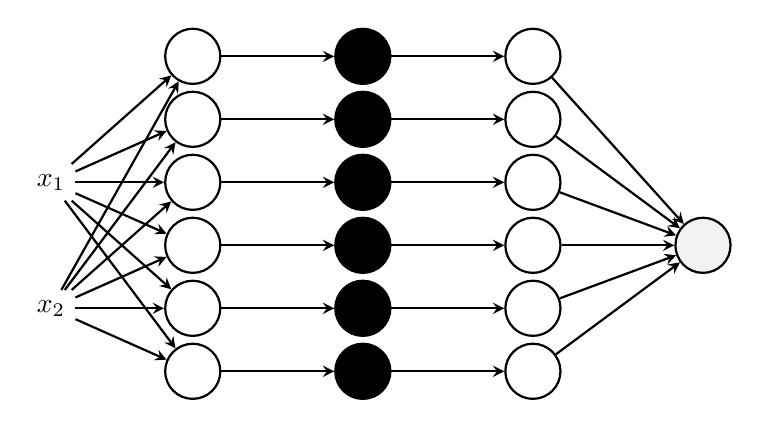
\begin{tikzpicture}[x=1.8cm, y=0.8cm, >=stealth, thick]

% Input layer (2 neurons)
\node at (0,1) (x1) {$x_1$};
\node at (0,-1) (x2) {$x_2$};

% First hidden layer (6 neurons)
\foreach \i in {-2,-1,0,1,2,3} {
    \node[circle, draw, minimum size=0.7cm] (h1\i) at (1,\i) {};
    \draw[->] (x1) -- (h1\i);
    \draw[->] (x2) -- (h1\i);
}

% Middle layer — infinity (dots only)
\foreach \i in {-2,-1,0,1,2,3} {
    \node[circle, draw, minimum size=0.7cm, fill=black] (hd\i) at (2.2,\i) {};
}
\node at (2.2,1.7) {$\vdots$};
\node at (2.2,-1.7) {$\vdots$};

% Connect previous to dots
\foreach \i in {-2,-1,0,1,2,3} {
    \draw[->] (h1\i) -- (hd\i);
}

% Last hidden layer (6 neurons)
\foreach \i in {-2,-1,0,1,2,3} {
    \node[circle, draw, minimum size=0.7cm] (h3\i) at (3.4,\i) {};
    \draw[->] (hd\i) -- (h3\i);
}

% Output layer (1 neuron)
\node[circle, draw, minimum size=0.7cm, fill=gray!10] (out) at (4.6,0) {};
\foreach \i in {-2,-1,0,1,2,3} {
    \draw[->] (h3\i) -- (out);
}

\end{tikzpicture}
\caption{Fully connected network with infinitely many hidden layers (conceptual representation).}
\end{figure}

\vspace{2em}
\begin{center}
\LARGE \textbf{From Diagram to Code: Artificial Neural Network.}
\end{center}

You’ve now seen what a fully connected neural network looks like —  
from inputs to outputs, through multiple layers of neurons.  
Let’s now build it from scratch in code.

Our goal is simple:

\begin{quote}
\textbf{Create a neural network where we can define any number of layers and neurons.}
\end{quote}

No black boxes, no shortcuts.  
Just Python, NumPy, and clean mathematics.

\subsection*{Architecture Definition}

Before training a neural network, we need to define its architecture.

\bigskip

We need to answer two fundamental questions:

\begin{itemize}
  \item How many layers?
  \item How many neurons in each layer?
\end{itemize}

\medskip

To address this, we will create a function that initializes the parameters of our network.  
This function will encode both the number of layers and the number of neurons in each layer.

\medskip

Each layer $l$ will be associated with:
\begin{itemize}
  \item a weight matrix $\mathbf{W}^{[l]}$
  \item a bias vector $\mathbf{b}^{[l]}$
\end{itemize}

\medskip

These matrices are not arbitrary.  
Their dimensions tell us precisely how many neurons are present in each layer — and how each layer is connected to the previous one.

\bigskip

\noindent\textit{So how do we encode this architecture in code?}

\medskip

\noindent With a simple list.

\medskip

\begin{quote}
The \texttt{length} of the list tells us how many layers there are. \\
The \texttt{value at each index} tells us how many neurons are in that layer.
\end{quote}

\bigskip

A simple and expressive design.

Let’s now translate it into Python.


\vspace{0.5em}
Here is the initialization function:

\vspace{0.5em}
\begin{lstlisting}[language=Python, frame=single, caption=Initialisation of parameters, basicstyle=\ttfamily\small]
def initialisation(dimensions):
    parameters = {}
    L = len(dimensions)

    for l in range(1, L):
        parameters[f"W{l}"] = np.random.randn(dimensions[l], dimensions[l - 1])
        parameters[f"b{l}"] = np.random.randn(dimensions[l], 1)

    return parameters
\end{lstlisting}

\vspace{1em}

Note how the weights and biases are initialized randomly for each layer. But most importantly: how the \texttt{dimensions} list governs the shape of each weight and bias matrix.


The matrix $\mathbf{W}^{[l]}$ has shape $(\text{neurons in layer } l, \text{neurons in layer } l-1)$,
and the bias vector $\mathbf{b}^{[l]}$ has shape $(\text{neurons in layer } l, 1)$.

\vspace{1em}

We now define the shape of our neural network and use this function to initialize all parameters:

\vspace{0.5em}
\begin{lstlisting}[language=Python, frame=single, basicstyle=\ttfamily\small]
dimensions = [2, 32, 32, 1]
parameters = initialisation(dimensions)

for key, value in parameters.items():
    print(f"{key} {value.shape}")
\end{lstlisting}

\vspace{0.5em}

This produces the following output:

\begin{verbatim}
W1 (32, 2)
b1 (32, 1)
W2 (32, 32)
b2 (32, 1)
W3 (1, 32)
b3 (1, 1)
\end{verbatim}

\vspace{1em}

\noindent This output tells us:
\begin{itemize}
  \item The first layer has 32 neurons, each connected to the 2 input features.
  \item The second layer has 32 neurons, each connected to the previous layer's 32 neurons.
  \item The output layer has 1 neuron, connected to the last hidden layer's 32 neurons.
\end{itemize}

You have just defined a complete fully connected neural network.

\vspace{2em}
\begin{center}
\LARGE \textbf{Next step: Give it a purpose.}
\end{center}


\subsection*{Forward Propagation}

Let’s now bring this architecture to life.

\bigskip

\noindent
Recall from the previous notebook:  
Each layer takes as input the output of the previous one.  
The input layer receives the raw data $X$, while each subsequent layer receives the activation of the previous layer.

\medskip

We now generalize this behavior.

\begin{quote}
The $i$-th layer takes as input the activation $A^{[i-1]}$ from the previous layer, applies a linear transformation, and then passes it through a non-linear activation function.
\end{quote}

\medskip

At each layer $l$, we compute:
\[
Z^{[l]} = W^{[l]} A^{[l-1]} + b^{[l]}, \quad A^{[l]} = \sigma(Z^{[l]})
\]

\bigskip

This creates a chain-like structure where information flows from layer to layer, gradually transforming raw input into high-level features.

\medskip

Here is the function that implements this process:

\vspace{0.5em}
\begin{lstlisting}[language=Python, frame=single, caption=Forward propagation through all layers, basicstyle=\ttfamily\small]
def forward_propagation(X, parameters):
    activations = {}
    L = len(parameters) // 2  # total number of layers

    A = X
    activations['A0'] = A

    for l in range(1, L + 1):
        W = parameters[f'W{l}']
        b = parameters[f'b{l}']

        Z = np.dot(W, A) + b
        A = 1 / (1 + np.exp(-Z))  # sigmoid activation

        activations[f'A{l}'] = A

    return activations
\end{lstlisting}

\bigskip

We now run this function on our input data:

\vspace{0.5em}
\begin{lstlisting}[language=Python, frame=single, basicstyle=\ttfamily\small]
activations = forward_propagation(X, parameters)

for key, value in activations.items():
    print(key, value.shape)
\end{lstlisting}

\medskip

This produces the following output:

\begin{verbatim}
A0 (2, 100)
A1 (32, 100)
A2 (32, 100)
A3 (1, 100)
\end{verbatim}

\bigskip

\noindent Interpretation:
\begin{itemize}
  \item The input $X$ contains 100 examples with 2 features — hence $A^{[0]}$ has shape $(2, 100)$.
  \item The first and second hidden layers each have 32 neurons, and compute activations over all 100 examples — hence $(32, 100)$.
  \item The output layer has a single neuron — one prediction per example.
\end{itemize}

\vspace{2em}
\begin{center}
\LARGE \textbf{From raw data to prediction — layer by layer.}
\end{center}


\section*{Backpropagation}

Once the network computes a prediction, we need to measure how wrong it is — and more importantly, how to correct it.  
This is the role of \textbf{backpropagation}.

\bigskip

We start from the output layer and work backward, computing the gradients of the loss with respect to each parameter in the network.

\bigskip

Let’s begin with a concrete example: a network with two layers.

\[
\begin{aligned}
\frac{\partial \mathcal{L}}{\partial W_2} &= \frac{1}{m} (A_2 - Y) \cdot A_1^\top \\
\frac{\partial \mathcal{L}}{\partial b_2} &= \frac{1}{m} \sum_{i=1}^m (A_2 - Y)^{(i)} \\
\frac{\partial \mathcal{L}}{\partial W_1} &= \frac{1}{m} dZ_1 \cdot X^\top \\
\frac{\partial \mathcal{L}}{\partial b_1} &= \frac{1}{m} \sum_{i=1}^m dZ_1^{(i)}
\end{aligned}
\]

with:
\[
\begin{aligned}
dZ_2 &= A_2 - Y \\
dZ_1 &= (W_2^\top \cdot dZ_2) \circ A_1 \circ (1 - A_1)
\end{aligned}
\]

\bigskip

\textbf{Generalization to any layer $l$}

Take a moment to observe the pattern.  
Each layer computes its local error $dZ_l$ based on the error from the layer above and the derivative of its activation function.

\medskip

So for the last layer:
\[
dZ_L = A_L - Y
\]
and for all hidden layers $l < L$:
\[
dZ_l = (W_{l+1}^\top \cdot dZ_{l+1}) \circ A_l \circ (1 - A_l)
\]

\bigskip

That’s why, for any layer $l$ in a network of $L$ layers, we have:
\[
\begin{aligned}
\frac{\partial \mathcal{L}}{\partial W_l} &= \frac{1}{m} dZ_l \cdot A_{l-1}^\top \\
\frac{\partial \mathcal{L}}{\partial b_l} &= \frac{1}{m} \sum_{i=1}^m dZ_l^{(i)}
\end{aligned}
\]

\medskip

where:
\begin{itemize}
  \item $m$ is the number of training examples,
  \item $A_{l-1}$ is the activation from the previous layer,
  \item $dZ_l$ is the local error at layer $l$,
  \item $\circ$ denotes the element-wise (Hadamard) product.
\end{itemize}

\bigskip

\textbf{Backpropagation works by:}
\begin{enumerate}
    \item Computing the output error $dZ_L$
    \item Propagating it backward through the network using the weights and the sigmoid derivative
    \item Computing gradients $\frac{\partial \mathcal{L}}{\partial W_l}$ and $\frac{\partial \mathcal{L}}{\partial b_l}$ at each layer
    \item Using these gradients to update the parameters via gradient descent
\end{enumerate}


\newpage
Let’s now translate this logic into code:

\vspace{0.5em}
\begin{lstlisting}[language=Python, frame=single, caption=General backpropagation algorithm, basicstyle=\ttfamily\small]
def back_propagation(y, parameters, activations):
    m = y.shape[1]
    L = len(parameters) // 2
    dZ = activations[f'A{L}'] - y
    gradients = {}

    for l in reversed(range(1, L + 1)):
        A_prev = activations[f'A{l-1}']
        W = parameters[f'W{l}']

        gradients[f'dW{l}'] = (1/m) * np.dot(dZ, A_prev.T)
        gradients[f'db{l}'] = (1/m) * np.sum(dZ, axis=1, keepdims=True)

        if l > 1:
            dA_prev = np.dot(W.T, dZ)
            dZ = dA_prev * A_prev * (1 - A_prev)

    return gradients
\end{lstlisting}

\vspace{1em}

\noindent
Let’s unpack what just happened.

This function may look concise — but it captures the full elegance of the backpropagation algorithm.

\medskip

We begin at the output layer: $dZ = A_L - Y$ — the raw difference between prediction and ground truth. From there, we iterate backwards.  
At each layer, we compute the gradient of the loss with respect to the weights and biases using clean, vectorized expressions:
\[
\frac{\partial \mathcal{L}}{\partial W_l} = \frac{1}{m} dZ_l \cdot A_{l-1}^\top, \quad
\frac{\partial \mathcal{L}}{\partial b_l} = \frac{1}{m} \sum dZ_l
\]

Then comes the key insight: the chain rule.  
We take the upstream gradient and flow it backward through the weights:
\[
dA_{l-1} = W_l^\top \cdot dZ_l
\]
We then apply the derivative of the sigmoid function:
\[
dZ_{l-1} = dA_{l-1} \circ A_{l-1} \circ (1 - A_{l-1})
\]
This gives us the local error for the previous layer — and the cycle continues.

\medskip

\noindent
In just a few lines, we’ve implemented a fully general backpropagation engine — one that can scale to any depth, and prepare the ground for efficient learning via gradient descent.

\vspace{2em}
\begin{center}
\Large \textit{From abstract math to concrete code — this is the heart of learning.}
\end{center}


\bigskip

We now run the function and inspect the shape of each computed gradient:

\vspace{0.5em}
\begin{lstlisting}[language=Python, frame=single, basicstyle=\ttfamily\small]
gradients = back_propagation(y, parameters, activations)
for key, value in gradients.items():
    print(key, value.shape)
\end{lstlisting}

\bigskip

This produces the following output:

\begin{verbatim}
dW3 (1, 32)
db3 (1, 1)
dW2 (32, 32)
db2 (32, 1)
dW1 (32, 2)
db1 (32, 1)
\end{verbatim}

\bigskip

\noindent
Each gradient is shaped to exactly match the parameter it updates:

\begin{itemize}
  \item \textbf{Layer 3 (Output)} \\
  \texttt{dW3 (1, 32)} connects 32 activations from the last hidden layer to 1 output neuron \\
  \texttt{db3 (1, 1)} is the bias for the output neuron
  \medskip
  \item \textbf{Layer 2 (Hidden)} \\
  \texttt{dW2 (32, 32)} connects 32 neurons from layer 1 to 32 neurons in layer 2 \\
  \texttt{db2 (32, 1)} is the bias vector for each neuron in layer 2
  \medskip
  \item \textbf{Layer 1 (Hidden)} \\
  \texttt{dW1 (32, 2)} maps the input features (2-dimensional) to the first hidden layer (32 neurons) \\
  \texttt{db1 (32, 1)} is the bias vector for layer 1
\end{itemize}

\bigskip

This layout mirrors the structure of the network itself — from output to input.  
Each gradient flows in reverse order, ready to update the corresponding parameter in a single pass.

\medskip

\noindent
This is how learning happens: through structure, through precision, and through alignment between theory and implementation.

\medskip

\noindent
This is more than just a shape check — it’s a validation of the entire learning pipeline.

Every derivative, every matrix product, every layer — it all fits.  
The math and the code speak the same language.

\bigskip

Each gradient is now ready to be used for one purpose: to make the model better.


\newpage
\begin{center}
\LARGE \textbf{Backpropagation demystified. Time to use it.}
\end{center}


\section*{Gradient Descent: Updating the Parameters}

Backpropagation gave us the gradients — but gradients alone don’t change anything.

To improve the model, we need to update the parameters in the direction that reduces the loss.  
That’s what gradient descent does.

\bigskip

At each layer $l$, we perform the update:
\[
\begin{aligned}
W^{[l]} &\leftarrow W^{[l]} - \alpha \cdot \frac{\partial \mathcal{L}}{\partial W^{[l]}} \\
b^{[l]} &\leftarrow b^{[l]} - \alpha \cdot \frac{\partial \mathcal{L}}{\partial b^{[l]}}
\end{aligned}
\]

\medskip

\noindent Where $\alpha$ is the learning rate — a small scalar that controls the step size of the update.

\bigskip

Here is the Python function that applies this rule to every layer:

\vspace{0.5em}
\begin{lstlisting}[language=Python, frame=single, caption=Parameter update using gradient descent, basicstyle=\ttfamily\small]
def update_parameters(parameters, gradients, learning_rate):
    L = len(parameters) // 2

    for l in range(1, L + 1):
        parameters[f'W{l}'] -= learning_rate * gradients[f'dW{l}']
        parameters[f'b{l}'] -= learning_rate * gradients[f'db{l}']

    return parameters
\end{lstlisting}

\bigskip

This simple loop performs one update step across all layers.

\begin{itemize}
  \item \texttt{parameters} holds the current weights and biases
  \item \texttt{gradients} comes from backpropagation
  \item \texttt{learning\_rate} determines how fast (or slow) the model learns
\end{itemize}

\medskip

\noindent
Each parameter takes a small step in the direction that reduces the loss — bringing the network closer to a better set of predictions.

\newpage
\begin{center}
\LARGE \textbf{This is where the network becomes alive.}
\end{center}

\section*{Training Loop}

We now have all the pieces.

\begin{itemize}
  \item \textbf{Forward propagation} to make a prediction
  \item \textbf{Backpropagation} to compute the error and how to correct it
  \item \textbf{Gradient descent} to apply that correction
\end{itemize}

\noindent
Individually, they are just mechanisms.  
Together — they become something more.

\medskip
\textbf{It becomes the neural network.}

\medskip

And we train it using the same \textbf{training loop} that contains three steps:

\begin{enumerate}
  \item It receives input and computes an output.
  \item It evaluates how wrong it was.
  \item It rewires itself — slightly — to do better next time.
\end{enumerate}

Iteration after iteration, this cycle repeats.  
The weights shift. The loss decreases. The predictions improve.

\bigskip

Here is the code that brings the network to life:

\vspace{0.5em}
\begin{lstlisting}[language=Python, frame=single, caption=The training loop — where learning happens, basicstyle=\ttfamily\small]
def neural_network(X, y, dimensions, learning_rate=0.1, iterations=1000):
    parameters = initialisation(dimensions)

    for i in range(iterations):
        # Forward pass
        activations = forward_propagation(X, parameters)

        # Backward pass
        gradients = back_propagation(y, parameters, activations)

        # Parameter update
        parameters = update_parameters(parameters, gradients, learning_rate)

        # Optional: track the loss
        if i % 100 == 0:
            A_final = activations[f'A{len(dimensions) - 1}']
            loss = -np.mean(y * np.log(A_final) + (1 - y) * np.log(1 - A_final))
            print(f"Iteration {i}: loss = {loss:.4f}")

    return parameters
\end{lstlisting}

\bigskip

This is not just a loop.

It is a feedback system. An adaptive structure.  
A recursive engine that takes raw input and sculpts its own internal logic to match the world.

\medskip

\noindent
You can control how fast it learns (\texttt{learning\_rate}), how long it trains (\texttt{iterations}), or how deep and wide it thinks (\texttt{dimensions}).

But once launched, this function learns — by itself.


\section*{From Prediction to Decision: Toxic or Not?}

Let’s now return to our original goal:  
\textit{classify whether a plant is toxic or not, based on its features.}

\bigskip

To explore this, we will simulate a variety of synthetic datasets that represent labelled toxic (class 1) and non-toxic (class 0) plants.
For each one, we’ll let the neural network classify the inputs — and visualize the decision boundary it creates.

\begin{quote}
This is how we see what the network "thinks".\\
How it splits space. Where it draws the line. Literally.
\end{quote}

\bigskip

Here’s how we’ll do it:

\begin{enumerate}
  \item Generate a dataset (e.g. moons, circles, blobs, spirals)
  \item Train the neural network using our \texttt{neural\_network()} function
  \item Visualize the final decision surface: which regions are predicted toxic ($\hat{y} = 1$) and which are not ($\hat{y} = 0$)
\end{enumerate}

\medskip

The prediction itself is simple:

\vspace{0.5em}
\begin{lstlisting}[language=Python, frame=single, caption=Predicting class from probability, basicstyle=\ttfamily\small]
def predict(X, parameters):
    activations = forward_propagation(X, parameters)
    A_final = activations[f'A{len(parameters) // 2}']
    return (A_final >= 0.5)
\end{lstlisting}

\medskip

This function gives a final binary decision for each plant, based on the output activation.  
But what’s far more interesting — is the structure the network built to make that decision.

\bigskip

Let’s now visualize that internal geometry.  
We’ll paint the input space according to the model’s belief: toxic or not toxic.  
And then we’ll overlay the real data to see what the model understood.
\vspace{2em}
\begin{center}
\LARGE\bfseries The boundary is the belief. Let’s see how it thinks.
\end{center}

\vspace{1em}
\noindent Let’s try it on different datasets and see how the neural network adapts.

\section*{First Dataset: Random Blobs}

\vspace{0.5em}
We generate a synthetic binary classification problem using two clusters of points.

\begin{lstlisting}[language=Python]
X, y = make_blobs(n_samples=200, centers=2, random_state=42, cluster_std=1.5)
\end{lstlisting}

\begin{figure}[H]
    \centering
    \includegraphics[width=0.5\textwidth]{/Users/louispierre-c/Desktop/photos_git/dataset_1.png}
    \caption{Random Dataset — Leaf Width vs. Length}
    \label{fig:dataset}
\end{figure}

\vspace{1em}
We chose a two-hidden-layer neural network with 64 neurons in each layer:  
\begin{center}
\texttt{dimensions = [2, 64, 64, 1]}
\end{center}

And we train it with a learning rate of 0.1 for 500 epochs:
\vspace{0.5em}

\begin{lstlisting}[language=Python]
neural_network(X, y, [2, 64, 64, 1], learning_rate=0.1, epoch=500)
\end{lstlisting}

\vspace{0.5em}
Training progression:

\begin{figure}[H]
    \centering
    \includegraphics[width=1\textwidth]{/Users/louispierre-c/Desktop/photos_git/T12.png}
    \caption{Training Progress on Random Dataset}
    \label{fig:training_process}
\end{figure}

\vspace{0.5em}
And now, the decision boundary:

\begin{figure}[H]
    \centering
    \includegraphics[width=0.6\textwidth]{/Users/louispierre-c/Desktop/photos_git/T11.png}
    \caption{Decision Boundary for Random Dataset}
    \label{fig:decision_boundary}
\end{figure}

\section*{Second Dataset: Concentric Circles}

\vspace{0.5em}
This one’s harder. Two intertwined classes. Let’s see if the network can handle it.

\begin{lstlisting}[language=Python]
X, y = make_circles(n_samples=100, noise=0.1, factor=0.3, random_state=0)
neural_network(X, y, [2, 64, 64, 1], learning_rate=0.1, epoch=500)
\end{lstlisting}

\begin{figure}[H]
    \centering
    \includegraphics[width=0.6\textwidth]{/Users/louispierre-c/Desktop/photos_git/T13.png}
    \caption{Concentric Circles Dataset}
    \label{fig:circles_dataset}
\end{figure}

Longer training — more complexity:

\begin{lstlisting}[language=Python]
neural_network(X, y, [2, 64, 64, 1], learning_rate=0.1, epoch=5000)
\end{lstlisting}

\begin{figure}[H]
    \centering
    \includegraphics[width=1\textwidth]{/Users/louispierre-c/Desktop/photos_git/T14.png}
    \caption{Training Progress on Circles Dataset}
    \label{fig:circles_training}
\end{figure}

\vspace{0.5em}
Final decision boundary:

\begin{figure}[H]
    \centering
    \includegraphics[width=0.6\textwidth]{/Users/louispierre-c/Desktop/photos_git/T15.png}
    \caption{Decision Boundary for Circles Dataset}
    \label{fig:circles_boundary}
\end{figure}

\begin{center}
\itshape Now you understand the power of a neural network ?
\end{center}

\begin{quote}
\textbf{EVERY dataset can be classified now.}
\end{quote}

\noindent You now have an independant learning tool that classifies nearly any dataset.

\begin{center}
\Large \texttt{And you built it from scratch.}
\end{center}

\section*{Can this Neural Network understands Moons dataset?}

\begin{figure}[H]
    \centering
    \includegraphics[width=0.6\textwidth]{/Users/louispierre-c/Desktop/photos_git/T16.png}
    \caption{Moons Dataset}
\end{figure}

\begin{lstlisting}[language=Python]
neural_network(X, y, [2, 64, 64, 1], learning_rate=0.1, epoch=5000)
\end{lstlisting}

\begin{figure}[H]
    \centering
    \includegraphics[width=1\textwidth]{/Users/louispierre-c/Desktop/photos_git/T23.png}
    \caption{Training Progress on Moons Dataset}
\end{figure}

\bigskip

\begin{figure}[H]
    \centering
    \includegraphics[width=0.5\textwidth]{/Users/louispierre-c/Desktop/photos_git/T17.png}
    \caption{Decision Boundary for Moons Dataset}
\end{figure}

\vspace{0.5em}

Okay, I know what you’re thinking:  
\textit{“This is just a toy example. It’s too easy.”}

\section*{Fourth Dataset: Spirals}

Let’s now create a much more challenging dataset.  
Not linearly separable. Not even close. Spirals.

\begin{figure}[H]
    \centering
    \includegraphics[width=0.5\textwidth]{/Users/louispierre-c/Desktop/photos_git/T18.png}
    \caption{Spiral Dataset}
\end{figure}

We train the same 2-layer network on this data:

\begin{lstlisting}[language=Python]
neural_network(X, y, [2, 64, 64, 1], learning_rate=0.1, epoch=5000)
\end{lstlisting}

\begin{figure}[H]
    \centering
    \includegraphics[width=1\textwidth]{/Users/louispierre-c/Desktop/photos_git/T21.png}
    \caption{Learning Curves}
\end{figure}

The model tries, but...  
\textit{The accuracy remains low. Something’s off.}

\begin{figure}[H]
    \centering
    \includegraphics[width=0.6\textwidth]{/Users/louispierre-c/Desktop/photos_git/T19.png}
    \caption{Decision Boundary for Spiral Dataset – 2 Layers}
\end{figure}

\bigskip
We now face a limitation.  
The network can’t separate the spirals.

\medskip
What can we do?

\begin{itemize}
  \item Increase the number of \textbf{epochs}? Maybe.
  \item Increase the \textbf{learning rate}? Risky.
  \item \textbf{Add more neurons, more layers}? Now we’re talking.
\end{itemize}

\section*{Upgrading the Brain}

Let’s go from:  
\texttt{[2, 64, 64, 1]} to \texttt{[2, 128, 128, 128, 128, 1]}. That’s 4 hidden layers with 128 neurons each.

\begin{lstlisting}[language=Python]
neural_network(X, y, [2, 128, 128, 128, 128, 1], learning_rate=0.1, epoch=5000)
\end{lstlisting}

\begin{figure}[H]
    \centering
    \includegraphics[width=1\textwidth]{/Users/louispierre-c/Desktop/photos_git/T22.png}
    \caption{Learning Curves for Spiral Dataset – 4 Layers}
\end{figure}
\noindent
And now, the decision boundary:

\begin{figure}[H]
    \centering
    \includegraphics[width=0.6\textwidth]{/Users/louispierre-c/Desktop/photos_git/T20.png}
    \caption{Decision Boundary for Spiral Dataset – 4 Layers}
\end{figure}

\textit{Oh yeah, that worked.}

We just built a brain that understands spirals.
But do you know what that really means ?

\section*{A Neural Network: Our Creation}

A neural network is not just a collection of equations. It is a structure we designed, a brain we shaped, a structure we designed, a logic we taught.  

\vspace{0.5em}

Let’s take a moment to appreciate that.

\noindent
We control its complexity. We choose how deeply it can think. We are, in a sense, its creators.

\noindent
Maybe he thinks we’re gods. Maybe he's right.
Maybe it’s planning to create its own religion or something like that.  
For now, though…

\medskip
\centerline{\textbf{Let’s keep using it to classify datasets.}}


\section*{What About Performance?}

Sometimes — of course — the model is not perfect.  
But what matters is this: we can \textit{see} the network searching, adjusting, learning.  
Even when the decision boundary isn’t flawless, we witness the model thinking.

\medskip

\noindent
For example, let's say we reached a final training accuracy of 85\%.  
That’s a solid first step.

\begin{quote}
\textbf{But is 85\% good enough?}  
That depends entirely on your objective.
\end{quote}

\begin{itemize}
    \item For a self-driving car? \textcolor{gray}{→ Absolutely not.}
    \item For a toy classification task? \textcolor{gray}{→ Definitely yes.}
\end{itemize}

\bigskip

But let’s be cautious.

\medskip

\noindent
\textbf{Adding more layers and neurons doesn’t always help.}  
It can increase the capacity of the network — yes — but there are some downsides of course, this world is balanced.

\medskip

\noindent
For example, it can also make the model memorize even the noise in your data instead of learning the underlying patterns.

\medskip

This phenomenon is called \textbf{overfitting}.

\medskip

\noindent
Overfitting happens when a model performs very well on the training data,  
but poorly on unseen data.

\medskip

\textit{It’s like a student who memorizes past exams instead of understanding the subject.}

\bigskip

\noindent
That’s why, as we increase the complexity of our model,  
we must also develop tools to measure generalization:  
validation data, regularization, early stopping, and more.

\bigskip

\begin{center}
\Large \texttt{But that’s a story for other guides and topics.}
\end{center}



\section*{Final Point on Overfitting}

\noindent
At this point, you might be wondering:  
\textit{“What about the performance on the cat/dog dataset?”}

\bigskip

Let's see the final [1, 128, 128, 128, 128, 1] neural network on the cat/dog dataset we had :

\begin{lstlisting}[language=Python]
neural_network(X, y, [2, 128, 128, 128, 128, 1], learning_rate=0.1, epoch=5000)
\end{lstlisting}
\bigskip

\begin{figure}[H]
    \centering
    \includegraphics[width=1\textwidth]{/Users/louispierre-c/Desktop/photos_git/final.png}
    \caption{Training Progress on Cat/Dog Dataset}
    \label{fig:cat_dog_training}
\end{figure}

\noindent
We still have an overfitting problem.
\bigskip
\noindent

This is, in fact, a textbook case of \textbf{overfitting}.  
The neural network is simply too powerful for the data we have.

\bigskip

There is no trick here.  
\textbf{Every model will fail.}

\bigskip

But why?

\medskip

We now face one of the most fundamental, million-dollar questions in machine learning:

\begin{center}
    \textbf{Is the problem in the data, the model, or the training process?}
\end{center}

\bigskip

Let’s dissect this.

\smallskip
\noindent
Suppose the model is well-designed. Still, we observe poor performance on the test set.  
Then, the culprit is likely the data itself.

\bigskip

What does it mean for data to be 'not good enough'?

\begin{itemize}
  \item It might be too small.
  \item It might lack diversity.
  \item It might not capture the true complexity of the task.
\end{itemize}

\bigskip

\noindent
The cat/dog dataset is a perfect illustration.  
It contains only \textbf{1,000 images}—far too few to train a high-capacity neural network without overfitting.

\bigskip

And that’s precisely why this guide ends here.

\bigskip

\noindent
Don’t fall into the trap of thinking that every problem can be solved with a neural network.  
Don’t believe that the solution lies hidden in some mathematical trick, in a piece of code, or in someone else’s mind.

\bigskip

\noindent
\textbf{The solution is in the process.}

\medskip
\noindent
In how we define the problem.  
In how we choose, structure, and question the data.  
In the model we design.  
In the way we train, test, and deploy.  
In every iteration, and every lesson along the way.

\bigskip

That’s why a true data scientist is so valuable.  
Because they’ve walked the path—\textit{without shortcuts}.  
Because they understand that the value is not just in the answer, but in the journey to reach it.

\newpage
\bigskip
\begin{center}
\Huge\textbf{Let's stop here this journey.}
\end{center}

\section*{Conclusion}

\textbf{You can be proud of yourself.}\\
You’ve taken the lead in your own learning process. And that changes everything.

\bigskip

Now that I’ve lightened the candle, will you start the fire?

Take a moment. Reflect on what you've learned, the code you’ve written, the concepts you've absorbed. And then, look at this:

\begin{lstlisting}[language=Python, frame=single, caption=Neural Network with TensorFlow, basicstyle=\ttfamily\small]
model = tf.keras.models.Sequential([
    tf.keras.layers.Dense(64, activation='sigmoid', input_shape=(2,)),
    tf.keras.layers.Dense(64, activation='sigmoid'),
    tf.keras.layers.Dense(1, activation='sigmoid')
])
model.compile(optimizer='sgd', loss='binary_crossentropy', metrics=['accuracy'])
model.fit(X, y, epochs=500, batch_size=32)
\end{lstlisting}

\noindent
This is a neural network built with TensorFlow, the very same architecture we just implemented from scratch.
\bigskip
\noindent
In just a few lines of code, you see it all: the activation function (Sigmoid), the optimizer (Gradient Descent Algorithm), the architecture, the loss function (log_loss). It’s all there.

But now, you understand what's behind it.\\
Not just the \emph{how}. You’ve started understanding the \emph{why}.

\bigskip

\noindent
Because here’s the truth:

\begin{center}
\textbf{The point is not to use the best library.}\\
\textbf{The point is to understand the reason it exists.}
\end{center}

\medskip

That’s what makes a real data scientist. That’s what makes someone able to solve actual problems — not just benchmark datasets. That’s what makes you valuable. Rare. Expensive.

\medskip

You now know how to train a neural network from scratch, how to visualize its decisions, how to make it learn. You’ve built the muscle memory of forward propagation, of backpropagation, of gradient descent.

And more importantly: you’ve built your own mental model of it.

\bigskip

But remember:

\begin{center}
\textbf{This is just the beginning.}
\end{center}

\medskip

Understanding the internal mechanics is one level. But understanding \textbf{when}, \textbf{how}, and \textbf{why} to use it — that’s a whole new game.

That’s what my next course will be about: not just learning to code, but understanding what it means to \textbf{be} a data scientist.

\bigskip

You don’t need a degree. Not a bachelor's. Not a master's. Not an engineering school.

Sure, those paths offer structure — professors, exercises, projects, deadlines. But they don’t offer the one thing that matters most:

\begin{center}
\textbf{The decision to learn.\\
The discipline to keep going.}
\end{center}

And that’s what you’ve done.

You chose this path. You decided to learn — not because you had to, but because something inside told you it mattered.

\medskip

\noindent
I'm not here to offer you comfort.\\
I'm not here to sugarcoat your journey.

I'm here because — like you — I chose to act.\\
I went through schools, degrees, certifications. But the things that shaped me the most, I built them myself — in silence, with effort, late at night, when no one was watching.

\medskip

So ask yourself: what's harder?

Learning like everyone else and ending up like everyone else?

Or making the decision to learn for yourself — and becoming something else entirely?

\bigskip

\noindent
Let me put it simply.

\begin{quote}
Do you want to believe in success,\\
or follow the path that leads to it?
\end{quote}

\medskip

Everything you've done so far — it shouldn't define you. It should free you.

Becoming excellent at deep learning is powerful. But don’t stop there.

\medskip

\noindent
Go beyond excellence.\\
Go beyond the hype.

What will make the difference is what you did the moment you opened this notebook:

\begin{center}
\textbf{You took your situation into your own hands.}
\end{center}

\medskip

You’ve learned the \textit{what}. You’ve built the \textit{how}.\\
Now it’s time to chase the \textit{why}.

\bigskip

\noindent
So play the game.\\
Make the effort.\\
And see how far it can take you.

\bigskip

\begin{center}
\Huge\textbf{Only you can decide that.}
\end{center}



\end{document}